\documentclass[]{book}
\usepackage{lmodern}
\usepackage{amssymb,amsmath}
\usepackage{ifxetex,ifluatex}
\usepackage{fixltx2e} % provides \textsubscript
\ifnum 0\ifxetex 1\fi\ifluatex 1\fi=0 % if pdftex
  \usepackage[T1]{fontenc}
  \usepackage[utf8]{inputenc}
\else % if luatex or xelatex
  \ifxetex
    \usepackage{mathspec}
  \else
    \usepackage{fontspec}
  \fi
  \defaultfontfeatures{Ligatures=TeX,Scale=MatchLowercase}
\fi
% use upquote if available, for straight quotes in verbatim environments
\IfFileExists{upquote.sty}{\usepackage{upquote}}{}
% use microtype if available
\IfFileExists{microtype.sty}{%
\usepackage{microtype}
\UseMicrotypeSet[protrusion]{basicmath} % disable protrusion for tt fonts
}{}
\usepackage{hyperref}
\hypersetup{unicode=true,
            pdftitle={darthpack: An R package with DARTH's decision modeling coding framework},
            pdfauthor={DARTH},
            pdfborder={0 0 0},
            breaklinks=true}
\urlstyle{same}  % don't use monospace font for urls
\usepackage{natbib}
\bibliographystyle{apalike}
\usepackage{color}
\usepackage{fancyvrb}
\newcommand{\VerbBar}{|}
\newcommand{\VERB}{\Verb[commandchars=\\\{\}]}
\DefineVerbatimEnvironment{Highlighting}{Verbatim}{commandchars=\\\{\}}
% Add ',fontsize=\small' for more characters per line
\usepackage{framed}
\definecolor{shadecolor}{RGB}{248,248,248}
\newenvironment{Shaded}{\begin{snugshade}}{\end{snugshade}}
\newcommand{\KeywordTok}[1]{\textcolor[rgb]{0.13,0.29,0.53}{\textbf{#1}}}
\newcommand{\DataTypeTok}[1]{\textcolor[rgb]{0.13,0.29,0.53}{#1}}
\newcommand{\DecValTok}[1]{\textcolor[rgb]{0.00,0.00,0.81}{#1}}
\newcommand{\BaseNTok}[1]{\textcolor[rgb]{0.00,0.00,0.81}{#1}}
\newcommand{\FloatTok}[1]{\textcolor[rgb]{0.00,0.00,0.81}{#1}}
\newcommand{\ConstantTok}[1]{\textcolor[rgb]{0.00,0.00,0.00}{#1}}
\newcommand{\CharTok}[1]{\textcolor[rgb]{0.31,0.60,0.02}{#1}}
\newcommand{\SpecialCharTok}[1]{\textcolor[rgb]{0.00,0.00,0.00}{#1}}
\newcommand{\StringTok}[1]{\textcolor[rgb]{0.31,0.60,0.02}{#1}}
\newcommand{\VerbatimStringTok}[1]{\textcolor[rgb]{0.31,0.60,0.02}{#1}}
\newcommand{\SpecialStringTok}[1]{\textcolor[rgb]{0.31,0.60,0.02}{#1}}
\newcommand{\ImportTok}[1]{#1}
\newcommand{\CommentTok}[1]{\textcolor[rgb]{0.56,0.35,0.01}{\textit{#1}}}
\newcommand{\DocumentationTok}[1]{\textcolor[rgb]{0.56,0.35,0.01}{\textbf{\textit{#1}}}}
\newcommand{\AnnotationTok}[1]{\textcolor[rgb]{0.56,0.35,0.01}{\textbf{\textit{#1}}}}
\newcommand{\CommentVarTok}[1]{\textcolor[rgb]{0.56,0.35,0.01}{\textbf{\textit{#1}}}}
\newcommand{\OtherTok}[1]{\textcolor[rgb]{0.56,0.35,0.01}{#1}}
\newcommand{\FunctionTok}[1]{\textcolor[rgb]{0.00,0.00,0.00}{#1}}
\newcommand{\VariableTok}[1]{\textcolor[rgb]{0.00,0.00,0.00}{#1}}
\newcommand{\ControlFlowTok}[1]{\textcolor[rgb]{0.13,0.29,0.53}{\textbf{#1}}}
\newcommand{\OperatorTok}[1]{\textcolor[rgb]{0.81,0.36,0.00}{\textbf{#1}}}
\newcommand{\BuiltInTok}[1]{#1}
\newcommand{\ExtensionTok}[1]{#1}
\newcommand{\PreprocessorTok}[1]{\textcolor[rgb]{0.56,0.35,0.01}{\textit{#1}}}
\newcommand{\AttributeTok}[1]{\textcolor[rgb]{0.77,0.63,0.00}{#1}}
\newcommand{\RegionMarkerTok}[1]{#1}
\newcommand{\InformationTok}[1]{\textcolor[rgb]{0.56,0.35,0.01}{\textbf{\textit{#1}}}}
\newcommand{\WarningTok}[1]{\textcolor[rgb]{0.56,0.35,0.01}{\textbf{\textit{#1}}}}
\newcommand{\AlertTok}[1]{\textcolor[rgb]{0.94,0.16,0.16}{#1}}
\newcommand{\ErrorTok}[1]{\textcolor[rgb]{0.64,0.00,0.00}{\textbf{#1}}}
\newcommand{\NormalTok}[1]{#1}
\usepackage{longtable,booktabs}
\usepackage{graphicx,grffile}
\makeatletter
\def\maxwidth{\ifdim\Gin@nat@width>\linewidth\linewidth\else\Gin@nat@width\fi}
\def\maxheight{\ifdim\Gin@nat@height>\textheight\textheight\else\Gin@nat@height\fi}
\makeatother
% Scale images if necessary, so that they will not overflow the page
% margins by default, and it is still possible to overwrite the defaults
% using explicit options in \includegraphics[width, height, ...]{}
\setkeys{Gin}{width=\maxwidth,height=\maxheight,keepaspectratio}
\IfFileExists{parskip.sty}{%
\usepackage{parskip}
}{% else
\setlength{\parindent}{0pt}
\setlength{\parskip}{6pt plus 2pt minus 1pt}
}
\setlength{\emergencystretch}{3em}  % prevent overfull lines
\providecommand{\tightlist}{%
  \setlength{\itemsep}{0pt}\setlength{\parskip}{0pt}}
\setcounter{secnumdepth}{5}
% Redefines (sub)paragraphs to behave more like sections
\ifx\paragraph\undefined\else
\let\oldparagraph\paragraph
\renewcommand{\paragraph}[1]{\oldparagraph{#1}\mbox{}}
\fi
\ifx\subparagraph\undefined\else
\let\oldsubparagraph\subparagraph
\renewcommand{\subparagraph}[1]{\oldsubparagraph{#1}\mbox{}}
\fi

%%% Use protect on footnotes to avoid problems with footnotes in titles
\let\rmarkdownfootnote\footnote%
\def\footnote{\protect\rmarkdownfootnote}

%%% Change title format to be more compact
\usepackage{titling}

% Create subtitle command for use in maketitle
\providecommand{\subtitle}[1]{
  \posttitle{
    \begin{center}\large#1\end{center}
    }
}

\setlength{\droptitle}{-2em}

  \title{darthpack: An R package with DARTH's decision modeling coding framework}
    \pretitle{\vspace{\droptitle}\centering\huge}
  \posttitle{\par}
  \subtitle{Supplementary Material to ``A need for change! A coding framework for
improving transparency in decision modeling''}
  \author{DARTH}
    \preauthor{\centering\large\emph}
  \postauthor{\par}
      \predate{\centering\large\emph}
  \postdate{\par}
    \date{2019-07-21}

\usepackage{booktabs}
\usepackage{float}
\usepackage{setspace}\onehalfspacing
\usepackage[margin=1in]{geometry}

\begin{document}
\maketitle

{
\setcounter{tocdepth}{1}
\tableofcontents
}
\chapter*{The Sick-Sicker model}\label{the-sick-sicker-model}
\addcontentsline{toc}{chapter}{The Sick-Sicker model}

In this case-study, we perform a cost-effectiveness analysis (CEA) using
a previously published 4-state model called the Sick-Sicker model
\citep{Enns2015}. In the Sick-Sicker model, a hypothetical disease
affects individuals with an average age of 25 years and results in
increased mortality, increased treatment costs and reduced quality of
life (QoL). We simulate this hypothetical cohort of 25-year-old
individuals over a lifetime (i.e., reaching an age of 100 years old)
using 75 annual cycles, represented with \texttt{n\_t}. The cohort
starts in the ``Healthy'' health state (denoted ``H''). Healthy
individuals are at risk of developing the illness, at which point they
would transition to the first stage of the disease (the ``Sick'' health
state, denoted ``S1''). Sick individuals are at risk of further
progressing to a more severe stage (the ``Sicker'' health state, denoted
``S2''), which is a constant probability in this case-study. There is a
chance that individuals in the Sick state eventually recover and return
back to the Healthy state. However, once an individual reaches the
Sicker state, they cannot recover; that is, the probability of
transitioning to the Sick or Healthy states from the Sicker state is
zero. Individuals in the Healthy state face background mortality that is
age-specific (i.e., time-dependent). Sick and Sicker individuals face an
increased mortality expressed as a hazard rate ratio (HR) of 3 and 10,
respectively, on the background mortality rate. Sick and Sicker
individuals also experience increased health care costs and reduced QoL
compared to healthy individuals. Once simulated individuals die, they
transition to the ``Dead'' state (denoted ``D''), where they remain.
Figure \ref{fig:STM-Sick-Sicker} shows the state-transition diagram of
the Sick-Sicker model. The evolution of the cohort is simulated in
one-year discrete-time cycles. Both costs and quality-adjusted life
years (QALYs) are discounted at an annual rate of 0.03\%.

\begin{figure}

{\centering 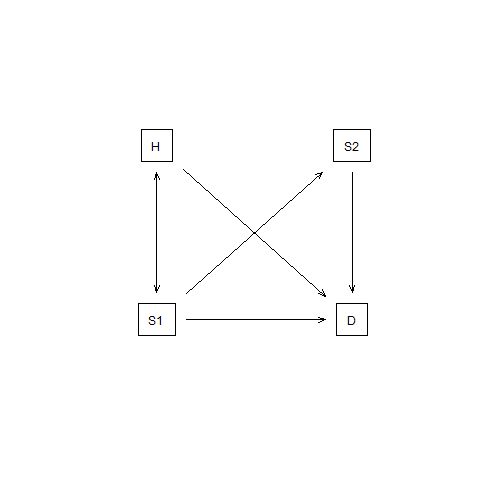
\includegraphics[width=6.67in]{../figs/02_model_diagram} 

}

\caption{State-transition diagram of the Sick-Sicker model. Healthy individuals can get Sick, die or stay healthy. Sick individuals can recover, transitioning back to healthy, can die, or stay sick. Once individuals are Sicker, they stay Sicker until they die.}\label{fig:STM-Sick-Sicker}
\end{figure}

Two alternative strategies exist for this hypothetical disease: a
no-treatment and a treatment strategy. Under the treatment strategy,
Sick and Sicker individuals receive treatment and continue doing so
until they recover or die. The cost of the treatment is additional to
the cost of being Sick or Sicker for one year. The treatment improves
QoL for those individuals who are Sick but has no effect on the QoL of
those who are sicker. To evaluate these two alternative strategies, we
perform a CEA.

We assume that most of the parameters of the Sick-Sicker model and their
uncertainty have been previously estimated and are known to the analyst.
However, while we can identify those who are afflicted with the illness
through obvious symptoms, we can not easily distinguish those in the
Sick state from the those in the Sicker state. Thus, we can not directly
estimate state-specific mortality hazard rate ratios, nor do we know the
transition probability of progressing from Sick to Sicker. Therefore, we
calibrate the model to different epidemiological data. We internally
validated the calibrated model by comparing the predicted outputs from
the model evaluated at the calibrated parameters against the calibration
targets \citep[\citet{Goldhaber_Fiebert2010}]{Eddy2012}.

As part of the CEA, we conducted different deterministic sensitivity
analysis (SA), including one-way and two-way SA, and tornado plots. To
quantify the effect of parameter uncertainty on decision uncertainty, we
conducted a probabilistic sensitivity analysis (PSA) and reported our
uncertainty analysis results with a cost-effectiveness acceptability
curve (CEAC), cost-effectiveness acceptability frontier (CEAF) and
expected loss curves (ELC) \citep{Alarid-Escudero2019}. We also
conducted a value of information (VOI) analysis to determine whether
potential future research is needed to reduce parameter uncertainty. All
steps of the CEA will be described using the different components of the
framework.

\section*{Set-up}\label{set-up}
\addcontentsline{toc}{section}{Set-up}

This report is a supplementary material meant to guide you through the
\texttt{R} code of a fully functional decision model to showcase the
framework described by the \href{http://darthworkgroup.com/}{Decision
Analysis in R for Technologies in Health (DARTH) workgroup} in the
manuscript \emph{A need for change! A coding framework for improving
transparency in decision modeling}. The code of this analysis can be
downloaded from GitHub
(\url{https://github.com/DARTH-git/Decision-Modeling-Framework}). We
recommend downloading the case-study files as a single .zip file
containing all directories. Unzip the folder and save to your desired
directory. The framework is divided into different directories,
described in Table 1, that could be accessed from the RStudio project
\emph{Decision-Modeling-Framework.Rproj}. In this framework, you will
find multiple directories as described in Table 1 of the main
manuscript. We refer to the directory names of this framework and
scripts stored in these directories using \emph{italic} style. This
report is created with Markdown and is located in the \emph{reports}
directory of the framework. The figures for the case-study can be found
in the \emph{figs} directory, data required to conduct some of the
analyses of the different components are in the \emph{data} directory
and the \texttt{R} scripts with functions, are located in the \emph{R}
directory. The main \texttt{R} scripts that conduct the analyses of the
different components of the framework are stored in the \texttt{R}
directory. In this document we do not show all the \texttt{R} code we
refer to. Therefore, it is important to follow along while reading this
document.

\chapter{Define model inputs}\label{inputs}

As described in the main manuscript, in this first component we declare
all model input variables and set their values. The \texttt{R} script
running the analysis of this component is the \emph{01\_model-inputs.R}
file in the \texttt{analysis} directory.

The input to inform the values is divided in three categories: external,
estimated, and calibrated. The majority of the Sick-Sicker model
parameters are informed by external data. Only three parameter values
need to be estimated using model calibration.

In this component, we start with the general setup of the model,
specifying among others the time horizon, name and number of health
states, proportion of the cohort in each of the different health states
at the start of the simulation and discount rates. The next step is to
specify the external parameters. The initial model parameter values and
\texttt{R} variable names are presented in Table \ref{tab:parameters}.

\begin{longtable}[]{@{}lcc@{}}
\caption{\label{tab:parameters} Description of the initial parameters with
their \texttt{R} name and value of the Sick-Sicker
model.}\tabularnewline
\toprule
\textbf{Parameter} & \textbf{R name} & \textbf{Value}\tabularnewline
\midrule
\endfirsthead
\toprule
\textbf{Parameter} & \textbf{R name} & \textbf{Value}\tabularnewline
\midrule
\endhead
Time horizon (\(n_t\)) & \texttt{n\_t} & 75 years\tabularnewline
Names of health states (\(n\)) & \texttt{v\_n} & H, S1, S2,
D\tabularnewline
Annual discount rate (costs/QALYs) & \texttt{d\_c}/\texttt{d\_e} &
3\%\tabularnewline
Annual transition probabilities & &\tabularnewline
- Disease onset (H to S1) & \texttt{p\_HS1} & 0.15\tabularnewline
- Recovery (S1 to H) & \texttt{p\_S1H} & 0.5\tabularnewline
- Disease progression (S1 to S2) in the time-homogenous model &
\texttt{p\_S1S2} & 0.105\tabularnewline
Annual mortality & &\tabularnewline
- All-cause mortality (H to D) & \texttt{p\_HD} &
age-specific\tabularnewline
- Hazard rate ratio of death in S1 vs H & \texttt{hr\_S1} &
3\tabularnewline
- Hazard rate ratio of death in S2 vs H & \texttt{hr\_S2} &
3\tabularnewline
Annual costs & &\tabularnewline
- Healthy individuals & \texttt{c\_H} & \$2,000\tabularnewline
- Sick individuals in S1 & \texttt{c\_S1} & \$4,000\tabularnewline
- Sick individuals in S2 & \texttt{c\_S2} & \$15,000\tabularnewline
- Dead individuals & \texttt{c\_D} & \$0\tabularnewline
- Additional costs of sick individuals treated in S1 or S2 &
\texttt{c\_Trt} & \$12,000\tabularnewline
Utility weights & &\tabularnewline
- Healthy individuals & \texttt{u\_H} & 1.00\tabularnewline
- Sick individuals in S1 & \texttt{u\_S1} & 0.75\tabularnewline
- Sick individuals in S2 & \texttt{u\_S2} & 0.50\tabularnewline
- Dead individuals & \texttt{u\_D} & 0.00\tabularnewline
Intervention effect & &\tabularnewline
- Utility for treated individuals in S1 & \texttt{u\_Trt} &
0.95\tabularnewline
\bottomrule
\end{longtable}

Age-specific background mortality for healthy individuals is represented
by the US population in 2015 and obtained from the
\href{https://www.mortality.org}{Human Mortality database}. This
information is stored in the \emph{01\_all-cause-mortality.csv} file in
the \emph{data} directory. Based on this .csv file a vector with
mortality rates by age is created using the \texttt{load\_mort\_data}
function in the \emph{01\_model-inputs\_functions.R} script. This
function gives us the flexibility to easily import data from other
countries or years.

\begin{Shaded}
\begin{Highlighting}[]
\KeywordTok{print.function}\NormalTok{(load_mort_data) }\CommentTok{# print the function}
\end{Highlighting}
\end{Shaded}

\begin{verbatim}
## function(file = NULL){
##   # Load mortality data from file
##   if(!is.null(file)) {
##     df_r_mort_by_age <- read.csv(file = file)}
##   else{
##     df_r_mort_by_age <- all_cause_mortality
##   }
##   # Vector with mortality rates
##   v_r_mort_by_age  <- as.matrix(dplyr::select(df_r_mort_by_age, Total))
##   
##   return(v_r_mort_by_age)
## }
## <bytecode: 0x10d1d43f8>
## <environment: namespace:darthpack>
\end{verbatim}

Another function in the \emph{01\_model-inputs\_functions.R} script, is
the \texttt{load\_all\_parms} function. This function, which is actually
using the \texttt{load\_mort\_data} function, loads all parameters for
the decision model from multiple sources and creates a list that
contains all parameters and their values.

\begin{Shaded}
\begin{Highlighting}[]
\KeywordTok{print.function}\NormalTok{(load_all_params)  }\CommentTok{# print the function}
\end{Highlighting}
\end{Shaded}

\begin{verbatim}
## function(file.init = NULL,
##                             file.mort = NULL){ # User defined
##   #### Load initial set of initial parameters form .csv file ####
##   if(!is.null(file.init)) {
##     df_params_init <- read.csv(file = file)
##   } else{
##     df_params_init <- df_params_init
##   }
##   
##   #### All-cause age-specific mortality from .csv file ####
##   v_r_mort_by_age <- load_mort_data(file = file.mort)
##   
##   l_params_all <- with(as.list(df_params_init), {
##     #### General setup ####
##     v_names_str <- c("No Treatment", "Treatment")  # CEA strategies
##     n_str       <- length(v_names_str) # Number of strategies
##     v_age_names <- n_age_init:(n_age_init + n_t - 1) # vector with age names
##     v_n <- c("H", "S1", "S2", "D")  # vector with the 4 health states of the model:
##                                     # Healthy (H), Sick (S1), Sicker (S2), Dead (D)
##     n_states <- length(v_n)         # number of health states 
##     v_s_init <- c(H = 1, S1 = 0, S2 = 0, D = 0) # initial state vector
##     #### Create list with all parameters ####
##     l_params_all <- list(
##       v_names_str = v_names_str,
##       n_str       = n_str      ,
##       n_age_init  = n_age_init, 
##       n_t         = n_t       , 
##       v_age_names = v_age_names,
##       v_n = v_n,
##       n_states = n_states,
##       v_s_init = c(H = 1, S1 = 0, S2 = 0, D = 0),
##       v_r_mort_by_age = v_r_mort_by_age
##     )
##     return(l_params_all)
##   }
##   )
##   
##   l_params_all <- c(l_params_all, 
##                     df_params_init) # Add initial set of parameters
## }
## <bytecode: 0x10d1c3118>
## <environment: namespace:darthpack>
\end{verbatim}

The \texttt{load\_all\_params} function is informed by the arguments
\texttt{file.init} and \texttt{file.mort}. The \texttt{file.init}
argument is a string with the location and name of the file with initial
set of parameters. The initial parameter values for our case-study are
stored in the \emph{01\_init-params.csv} file located in the \emph{data}
directory. The \texttt{load\_all\_params} function read this .csv file
into the function environment as a dataframe called,
\texttt{df\_params\_init}.

The \texttt{file.mort} argument is a string with the location and name
of the file with mortality data. As described before, in our case-study
this is the \emph{01\_all-cause-mortality.csv} file. Within the
\texttt{load\_all\_parms} function, the \texttt{load\_mort\_data}
function is used to create a vector with mortality rates from the .csv
data.

After loading all the information, the \texttt{load\_all\_params}
generates a list called,\texttt{l\_params\_all}, including all
parameters for the model including the general setup parameters and the
vector of mortality rates. The function also stores the dataframe
\texttt{df\_params\_init} with the initial set of parameters in the
list. This is all executed in the in the \emph{01\_model-inputs.R}
script by running the code below.

\begin{Shaded}
\begin{Highlighting}[]
\NormalTok{l_params_all <-}\StringTok{ }\KeywordTok{load_all_params}\NormalTok{()}
\end{Highlighting}
\end{Shaded}

For the Sick-Sicker model we do not have to estimate parameters, but we
do have three parameters that need to be estimated via model
calibration. In this stage of the framework, we simply set these
parameters to valid ``dummy'' values that are compatible with the next
phase of the analysis, model implementation, but are ultimately just
placeholder values until we conduct the calibration phase. This means
that these values will be replaced by the best-fitted calibrated values
after we performed the calibration in component 3.

Using a function to create a list of base-case parameters to have all
model parameters in a single object is very useful, because this object
will have to be updated for the calibration and the different
sensitivity analyses in components 3 and 5 of the framework,
respectively. Below, we guide you through the components of the
function.

\chapter{Decision model}\label{simulation}

In this second component, we build the backbone of the decision
analysis: the implementation of the model. This component is performed
by the \emph{02\_simulation\_model.R} script. This file itself is not
very large. It simply loads some packages and sources the input from
component 01 and in addition it runs the \texttt{decision\_model}
function that is used to caputre the dynamic process of the Sick-Sicker
example and stores the output. The output of the model is the
traditional cohort trace. The trace describes how the cohort is
distributed among the different health states over time and is plotted
at the end of this script.

The function \texttt{decision\_model} is defined in the
\emph{02\_simulation\_model\_functions.R} file in the \texttt{R} folder.
As described in the paper, constructing a model as a function at this
stage facilitates subsequent stages of the model development and
analysis. This since these processes will all call the same model
function, but pass different parameter values and/or calculate different
final outcomes based on the model outputs. In the next part, we will
describe the code within the function.

\begin{Shaded}
\begin{Highlighting}[]
\KeywordTok{print.function}\NormalTok{(decision_model) }\CommentTok{# print the code of the function}
\end{Highlighting}
\end{Shaded}

\begin{verbatim}
## function(l_params_all, err_stop = FALSE, verbose = FALSE){ # User defined
##   ### Definition:
##   ##   Decision model implementation function
##   ### Arguments:  
##   ##   l_params_all: List with all parameters of decision model
##   ##   verbose: Logical variable to indicate print out of messages
##   ### Returns:
##   ##   a_P: Transition probability array
##   ##   m_M: Matrix cohort trace
##   ##
##   with(as.list(l_params_all), {
##     #### Error checking ####
##     if ((n_t + n_age_init) > nrow(v_r_mort_by_age)) {
##       stop("Not all the age in the age range have a corresponding mortality rate")
##     }
##     
##     if ((sum(v_s_init) != 1) | !all(v_s_init >= 0)) {
##       stop("vector of initial states (v_s_init) is not valid")
##     }
## 
##     #### Age-specific transition probabilities ####
##     # Mortality for healthy individuals
##     p_HDage  <- 1 - exp(-v_r_mort_by_age[(n_age_init + 1) + 0:(n_t - 1)])        
##     # Mortality for sick individuals
##     p_S1Dage <- 1 - exp(-v_r_mort_by_age[(n_age_init + 1) + 0:(n_t - 1)] * hr_S1)
##     # Mortality for sicker individuals
##     p_S2Dage <- 1 - exp(-v_r_mort_by_age[(n_age_init + 1) + 0:(n_t - 1)] * hr_S2)
##     
##     #### Create age-specific transition probability matrices in an array ####
##     # Initialize array
##     a_P <- array(0, dim = c(n_states, n_states, n_t),
##                  dimnames = list(v_n, v_n, 0:(n_t-1)))
##     # Fill in array
##     # From H
##     a_P["H", "H", ]  <- (1-p_HDage) * (1 - p_HS1)
##     a_P["H", "S1", ] <- (1-p_HDage) * p_HS1
##     a_P["H", "D", ]  <- p_HDage
##     # From S1
##     a_P["S1", "H", ]  <- (1-p_S1Dage) * p_S1H
##     a_P["S1", "S1", ] <- (1-p_S1Dage) * (1 - (p_S1S2 + p_S1H))
##     a_P["S1", "S2", ] <- (1-p_S1Dage) * p_S1S2
##     a_P["S1", "D", ]  <- p_S1Dage
##     # From S2
##     a_P["S2", "S2", ] <- 1 - p_S2Dage
##     a_P["S2", "D", ]  <- p_S2Dage
##     # From D
##     a_P["D", "D", ] <- 1
##     
##     #### Check if transition array is valid ####
##     check_transition_probability(a_P, err_stop = err_stop, verbose = verbose)
##     check_sum_of_transition_array(a_P, n_states, n_t, err_stop = err_stop, verbose = verbose)
##     
##     #### Compute cohort trace matrix and transition array for age-dependent STM ####
##     # Initialize cohort trace matrix
##     m_M <- matrix(0, 
##                   nrow = (n_t + 1), ncol = n_states, 
##                   dimnames = list(0:n_t, v_n))
##     # Set first row of m.M with the initial state vector
##     m_M[1, ] <- v_s_init
##     
##     # Iterate STM over time
##     for(t in 1:n_t){
##       m_M[t + 1, ] <- m_M[t, ] %*% a_P[, , t]
##     }
##     return(list(a_P = a_P,
##                 m_M = m_M))
##   }
##   )
## }
## <bytecode: 0x109a97998>
## <environment: namespace:darthpack>
\end{verbatim}

The \texttt{decision\_model} function is informed by the argument
\texttt{l\_params\_all}. Via this argument we give the function a list
with all parameters of the decision model. For the Sick-Sicker model,
these parameters are stored in the list \texttt{l\_params\_all}, which
we passed into the function as shown below.

\begin{Shaded}
\begin{Highlighting}[]
\NormalTok{l_out_stm <-}\StringTok{ }\KeywordTok{decision_model}\NormalTok{(}\DataTypeTok{l_params_all =}\NormalTok{ l_params_all) }\CommentTok{# run the function}
\end{Highlighting}
\end{Shaded}

This function itself has all the mathematical equations of the decision
models coded inside. It starts by calculating the age-specific
transition probabilities from all non-dead states based on the vector of
age-specific mortality rates \texttt{v\_r\_mort\_by\_age}. These
parameters will become vectors of length \texttt{n\_t}, describing the
probability to die for all ages from all non-dead states.

The next part of the function, creates an array that stores age-specific
transition probability matrices in each of the third dimension. The
transition probability matrix is a core component of a state-transition
cohort model \citep{Iskandar2018}. This matrix contains the
probabilities of transitioning from the current health state, indicated
by the rows, to the other health states, specified by the columns. Since
we have age-specific transition probabilities, the transition
probability matrix is different each cycle. These probabilities are only
depending on the age of the cohort, and not on other events; therefore,
we can generate all matrices at the start of the model. This results in
\texttt{n\_t} different age-specific matrices that are stored in an
array, called \texttt{a\_P}, of dimensions \texttt{n\_states} x
\texttt{n\_states} x \texttt{n\_t}. After initializing the array, it is
filled with the transition probability stored in the list. When running
the model, we can index the correct transition probability matrix
corresponding with the current age of the cohort. We then added some
sanity checks to make sure that the transition matrices and the
transition probabilities are valid. The first three and last cycles of
the transition probability matrices stored in the array \texttt{a.P} are
shown below.

\begin{Shaded}
\begin{Highlighting}[]
\NormalTok{l_out_stm}\OperatorTok{$}\NormalTok{a_P[, , }\DecValTok{1}\OperatorTok{:}\DecValTok{3}\NormalTok{] }\CommentTok{# show the first three time-points of a_P}
\end{Highlighting}
\end{Shaded}

\begin{verbatim}
## , , 0
## 
##            H        S1        S2           D
## H  0.8491385 0.1498480 0.0000000 0.001013486
## S1 0.4984813 0.3938002 0.1046811 0.003037378
## S2 0.0000000 0.0000000 0.9899112 0.010088764
## D  0.0000000 0.0000000 0.0000000 1.000000000
## 
## , , 1
## 
##            H        S1        S2            D
## H  0.8491513 0.1498502 0.0000000 0.0009985012
## S1 0.4985037 0.3938180 0.1046858 0.0029925135
## S2 0.0000000 0.0000000 0.9900597 0.0099402657
## D  0.0000000 0.0000000 0.0000000 1.0000000000
## 
## , , 2
## 
##            H        S1        S2           D
## H  0.8490910 0.1498396 0.0000000 0.001069428
## S1 0.4983976 0.3937341 0.1046635 0.003204853
## S2 0.0000000 0.0000000 0.9893570 0.010642959
## D  0.0000000 0.0000000 0.0000000 1.000000000
\end{verbatim}

\begin{Shaded}
\begin{Highlighting}[]
\NormalTok{l_out_stm}\OperatorTok{$}\NormalTok{a_P[, , l_params_all}\OperatorTok{$}\NormalTok{n_t] }\CommentTok{# show it for the last cycle}
\end{Highlighting}
\end{Shaded}

\begin{verbatim}
##            H        S1         S2         D
## H  0.6055199 0.1068564 0.00000000 0.2876237
## S1 0.1807584 0.1427991 0.03795926 0.6384833
## S2 0.0000000 0.0000000 0.03365849 0.9663415
## D  0.0000000 0.0000000 0.00000000 1.0000000
\end{verbatim}

By comparing these probability matrices, we observe an increase in the
probabilities of transitioning to death from all health states.

After the array is filled, the cohort trace matrix, \texttt{m\_M}, of
dimensions \texttt{n\_t} x \texttt{n\_states} is initialized. This
matrix will store the state occupation at each point in time. The first
row of the matrix is informed by the initial state vector
\texttt{v\_s\_init}. For the remaining points in time, we iteratively
multiply the cohort trace with the age-specific transition probability
matrix corresponding to the specific cycle obtained by indexing the
array \texttt{a\_P} appropriately. All the outputs and relevant elements
of the decision model are stored in a list, called \texttt{l\_out\_stm}.
This list contains the array of the transition probability matrix for
all cycles \texttt{t} and the cohort trace \texttt{m\_M}.

\begin{Shaded}
\begin{Highlighting}[]
\KeywordTok{head}\NormalTok{(l_out_stm}\OperatorTok{$}\NormalTok{m_M)    }\CommentTok{# show the top part of the cohort trace}
\end{Highlighting}
\end{Shaded}

\begin{verbatim}
##           H        S1         S2           D
## 0 1.0000000 0.0000000 0.00000000 0.000000000
## 1 0.8491385 0.1498480 0.00000000 0.001013486
## 2 0.7957468 0.1862564 0.01568695 0.002309774
## 3 0.7684912 0.1925699 0.03501425 0.003924648
## 4 0.7484793 0.1909659 0.05478971 0.005765035
## 5 0.7306193 0.1873106 0.07413838 0.007931783
\end{verbatim}

\begin{Shaded}
\begin{Highlighting}[]
\KeywordTok{tail}\NormalTok{(l_out_stm}\OperatorTok{$}\NormalTok{m_M)    }\CommentTok{# show the bottom part of the cohort trace}
\end{Highlighting}
\end{Shaded}

\begin{verbatim}
##              H           S1           S2         D
## 70 0.009928317 0.0022433565 2.035951e-04 0.9876247
## 71 0.007153415 0.0015935925 1.311619e-04 0.9911218
## 72 0.005058845 0.0011174473 8.674540e-05 0.9937370
## 73 0.003460336 0.0007552206 5.436484e-05 0.9957301
## 74 0.002289594 0.0004937081 3.298632e-05 0.9971837
## 75 0.001475636 0.0003151589 1.985106e-05 0.9981894
\end{verbatim}

Using the code below, we can graphically show the model dynamics by
plotting the cohort trace. Figure \ref{fig:Sick-Sicker-Trace} shows the
distribution of the cohort among the different health states at each
time point.

\begin{figure}[H]

{\centering 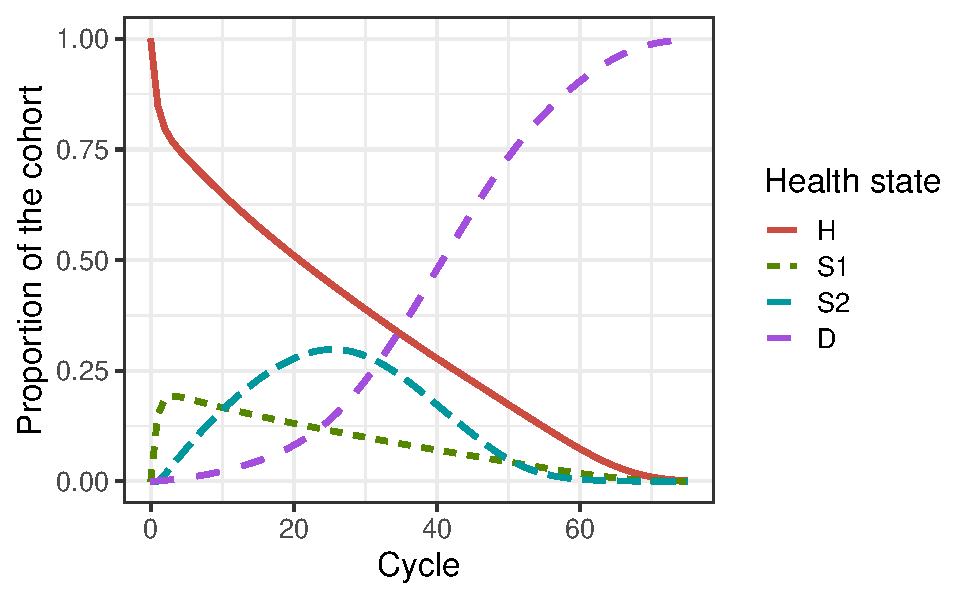
\includegraphics{report_files/figure-latex/Sick-Sicker-Trace-1} 

}

\caption{Cohort trace of the Sick-Sicker cohort model}\label{fig:Sick-Sicker-Trace}
\end{figure}

\chapter{Model calibration}\label{calibration}

In this third component, we calibrate unknown model parameters by
matching model outputs to specified calibration targets. Specifically,
we calibrate the Sick-Sicker model to match survival, prevalence and the
proportion who are Sicker, among all those afflicted (Sick+Sicker). We
used a Bayesian calibration approach using the incremental mixture
importance sampling (IMIS) algorithm \citep{Steele2006}, which has been
used to calibrate health policy models \citep[\citet{Menzies2017},
\citet{Rutter2018}]{Raftery2010}. Bayesian methods allow us to quantify
the uncertainty in the calibrated parameters even in the presence of
non-identifiability \citep{Alarid-Escudero2018b}. This analysis is coded
in the \emph{03\_calibration.R} file in the \texttt{analysis} folder.
The target data is stored in the \emph{03\_calibration\_targets.RData}
file. Similar to component 02 \ref{simulation}, in the section
\emph{03.1 Load packages}, we start by loading inputs and functions. In
addition, we load the calibration targets data into the R workspace. In
the next section, \emph{03.2 Visualize targets}, we plot each of the
calibration targets with their confidence intervals.

In section \emph{03.3 Run calibration algorithms}, we set the parameters
we need to calibrate to fixed values and test if the function
\texttt{calibration\_out} that produces model outputs corresponding to
the calibration targets works. This function takes a vector of
parameters that need to be calibrated and a list with all parameters of
decision model and computes model outputs to be used for calibration
routines.

\begin{Shaded}
\begin{Highlighting}[]
\KeywordTok{print.function}\NormalTok{(calibration_out) }\CommentTok{# print the functions}
\end{Highlighting}
\end{Shaded}

\begin{verbatim}
## function(v_params_calib, l_params_all){ # User defined
##   # Substitute values of calibrated parameters in base-case with 
##   # calibrated values
##   l_params_all <- update_param_list(l_params_all = l_params_all, params_updated = v_params_calib)
##   
##   # Run model with updated calibrated parameters
##   l_out_stm <- decision_model(l_params_all = l_params_all)
##   
##   ####### Epidemiological Output ###########################################
##   #### Overall Survival (OS) ####
##   v_os <- 1 - l_out_stm$m_M[, "D"]
##   
##   #### Disease prevalence #####
##   v_prev <- rowSums(l_out_stm$m_M[, c("S1", "S2")])/v_os
##   
##   #### Proportion of sick in S1 state #####
##   v_prop_S2 <- l_out_stm$m_M[, "S2"] / rowSums(l_out_stm$m_M[, c("S1", "S2")])
##   
##   ####### Return Output ###########################################
##   l_out <- list(Surv = v_os[c(11, 21, 31)],
##                 Prev = v_prev[c(11, 21, 31)],
##                 PropSicker = v_prop_S2[c(11, 21, 31)])
##   return(l_out)
## }
## <bytecode: 0x10d3bb690>
## <environment: namespace:darthpack>
\end{verbatim}

This function is informed by two argument \texttt{v\_params\_calib} and
\texttt{l\_params\_all}. The vector \texttt{v\_params\_calib} contains
the values of the three parameters of interest. The list
\texttt{l\_params\_all} contains all parameters of the decision model.
The placeholder values are replaced by \texttt{v\_params\_calib} and
with these values the model is evaluated. Model evaluation takes place
by running the \texttt{decision\_model} function, described in component
02. The result in a new list with output of the model corresponding to
the parameter values in the \texttt{v\_params\_calib}. With this new
decision model output, the overall survival, disease prevalence and the
proportion of Sicker in the Sick and Sicker states are calculated. The
estimated values for these epidemiological outcomes at different
timepoints are combined in a list called \texttt{l\_out} produced but
the \texttt{calibration\_out}.

Once we make sure this code works, we specify the calibration parameters
in section \emph{03.3.1 Specify calibration parameters}. These include
setting the seed for the random number generation, specifying the number
of random samples to obtain from the calibrated posterior distribution,
the name of the input parameters and the range of these parameters that
will inform the prior distributions of the calibrated parameters, and
the name of the calibration targets: \texttt{Surv}, \texttt{Prev},
\texttt{PropSick}.

In the next section, \emph{03.3.2 Run IMIS algorithm}, we calibrate the
Sick-Sicker model with the IMIS algorithm. For this case-study, we
assume a normal likelihood and uniform priors. For a more detailed
description of IMIS for Bayesian calibration, different likelihood
functions and prior distributions, we refer the reader to the tutorial
for Bayesian calibration by Menzies et al. \citep{Menzies2017}. We use
the \texttt{IMIS} function from the \texttt{IMIS} package that calls the
functions \texttt{likelihood}, \texttt{sample.prior} and \texttt{prior},
to draw samples from the posterior distribution \citep{IMIS}. The
functions are specified in the \emph{03\_calibration\_functions.R} file
in the \texttt{R} folder. For the \texttt{IMIS} function, we specify the
incremental sample size at each iteration of IMIS, the desired posterior
sample size at the resample stage, the maximum number of iterations in
IMIS and the number of optimizers which could be 0. The function returns
a list, which we call \texttt{l\_fit\_imis}, with the posterior samples,
the diagnostic statistics at each IMIS iteration and the centers of
Gaussian components \citep{IMIS}. We store the posterior samples in the
matrix \texttt{m\_calib\_post}.

We then explore these posterior distributions in section \emph{03.4
Exploring posterior distribution}. We start by estimating the posterior
mean, median and 95\% credible interval, the mode and the
maximum-a-posteriori (MAP). All for these summary statistics are
combined in a dataframe called \texttt{df\_posterior\_summ}. Table
\ref{tab:SummaryCal} shows the summary statistics of the posterior
distribution.

\begin{table}[t]

\caption{\label{tab:SummaryCal}Summary statistics of the posterior distribution}
\centering
\begin{tabular}{l|r|r|r|r|r|r}
\hline
  & Mean & 2.5\% & 50\% & 97.5\% & Mode & MAP\\
\hline
p\_S1S2 & 0.1076687 & 0.0964559 & 0.1073187 & 0.1196543 & 0.1067639 & 0.107841\\
\hline
hr\_S1 & 2.7261594 & 1.1010910 & 2.6790446 & 4.4020812 & 2.2857230 & 2.297053\\
\hline
hr\_S2 & 9.6232710 & 7.3427361 & 9.6461532 & 11.9533402 & 9.4629634 & 9.886776\\
\hline
\end{tabular}
\end{table}

In section \emph{03.4.2 Visualization of posterior distribution}, we
generate a pairwise scatter plot of the calibrated parameters (Figure
\ref{fig:03-posterior-distribution-marginal}) and a 3D scatter plot of
the joint posterior distribution (Figure
\ref{fig:Posterior-distribution-joint}). These figures are saved in the
\emph{figs} directory.

\begin{figure}

{\centering 
\includegraphics[width=33.33in]{../figs/03_posterior_distribution_joint} 

}

\caption{Joint posterior distribution}\label{fig:Posterior-distribution-joint}
\end{figure}

\begin{figure}

{\centering 
\includegraphics[width=33.33in]{../figs/03_posterior_distribution_marginal} 

}

\caption{Pairwise posterior distribution of calibrated parameters}\label{fig:03-posterior-distribution-marginal}
\end{figure}

Finally, the posterior distribution and MAP estimate from the IMIS
calibration are stored in the file \emph{03\_imis\_output.RData}.
Storing this data as an .Rdata file allows to import the data in
following sections without needing to re-run the calibration component.

\chapter{Validation}\label{validation}

In this forth component, we check the internal validity of our
Sick-Sicker model before we move on to the analysis components. To
internally validate the Sick-Sicker model, we compare the
model-predicted output evaluated at posterior parameters against the
calibration targets. This is all done in the \emph{04\_validation.R}
script in the \texttt{analysis} folder.

In section \emph{04.2 Compute model-predicted outputs}, we compute the
model-predicted outputs for each sample of posterior distribution as
well as for the MAP estimate. We then use the function
\texttt{data\_summary} to summarize the model-predicted posterior
outputs into different summary statistics.

\begin{Shaded}
\begin{Highlighting}[]
\KeywordTok{print.function}\NormalTok{(data_summary)}
\end{Highlighting}
\end{Shaded}

\begin{verbatim}
## function(data, varname, groupnames){
##   summary_func <- function(x, col){
##     c(mean = mean(x[[col]], na.rm = TRUE),
##       median = quantile(x[[col]], probs = 0.5, names = FALSE),
##       sd = sd(x[[col]], na.rm=TRUE),
##       lb = quantile(x[[col]], probs = 0.025, names = FALSE),
##       ub = quantile(x[[col]], probs = 0.975, names = FALSE))
##   }
##   data_sum <- plyr::ddply(data, groupnames, .fun = summary_func, 
##                     varname)
##   data_sum <- plyr::rename(data_sum, c("mean" = varname))
##   return(data_sum)
## }
## <bytecode: 0x10d41ca58>
## <environment: namespace:darthpack>
\end{verbatim}

This function is informed by three arguments, \texttt{data},
\texttt{varname} and \texttt{groupnames}.

The computation of the model-predicted outputs using the MAP estimate is
done by inserting the \texttt{v\_calib\_post\_map} data into the
previously described \texttt{calibration\_out} function. This function
creates a list including the estimated values for survival, prevalence
and the proportion of sicker individuals at cycles 10, 20 and 30.

In sections \emph{04.6 Internal validation: Model-predicted outputs
vs.~targets}, we check the internal validation by plotting the
model-predicted outputs against the calibration targets (Figures
\ref{fig:04-surv}-\ref{fig:04-proportion}). The generated plots are
saved as .png files in the \emph{fig} folder. These files can be used in
reports without the need of re-running the code.

\begin{figure}

{\centering 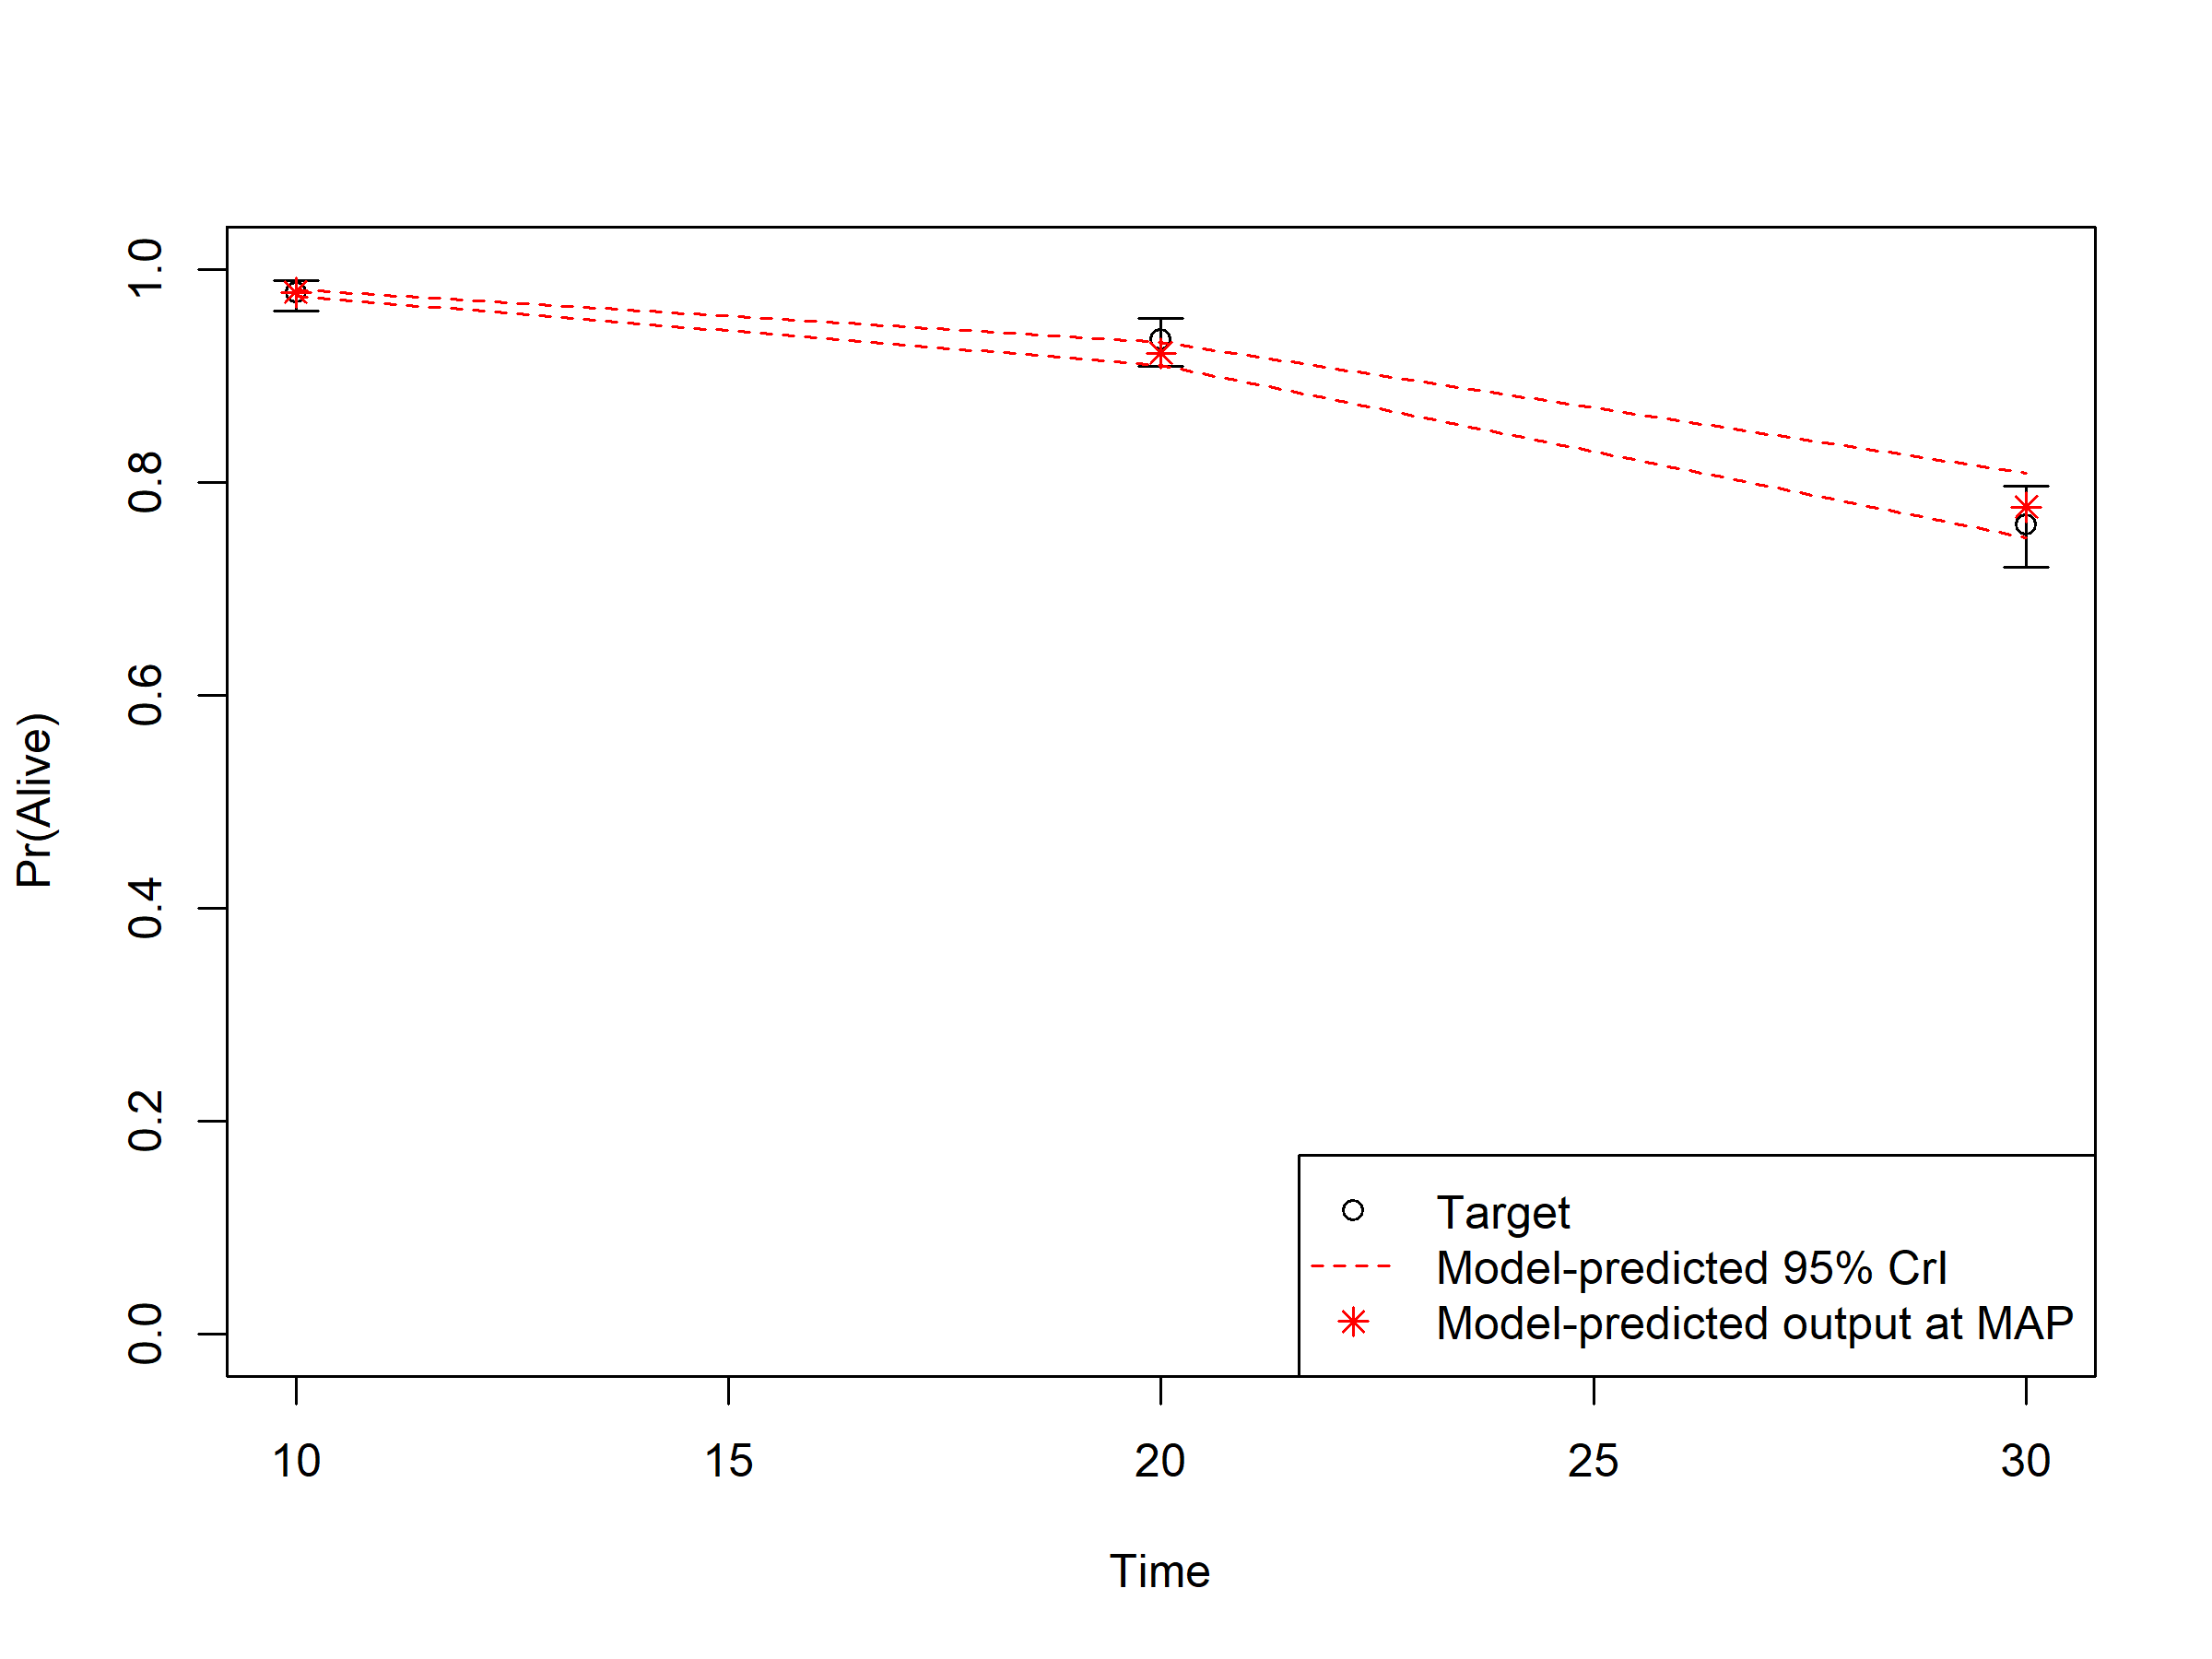
\includegraphics[width=33.33in]{../figs/04_posterior_vs_targets_survival} 

}

\caption{Survival data: Model-predicted outputs vs targets.}\label{fig:04-surv}
\end{figure}

\begin{figure}

{\centering 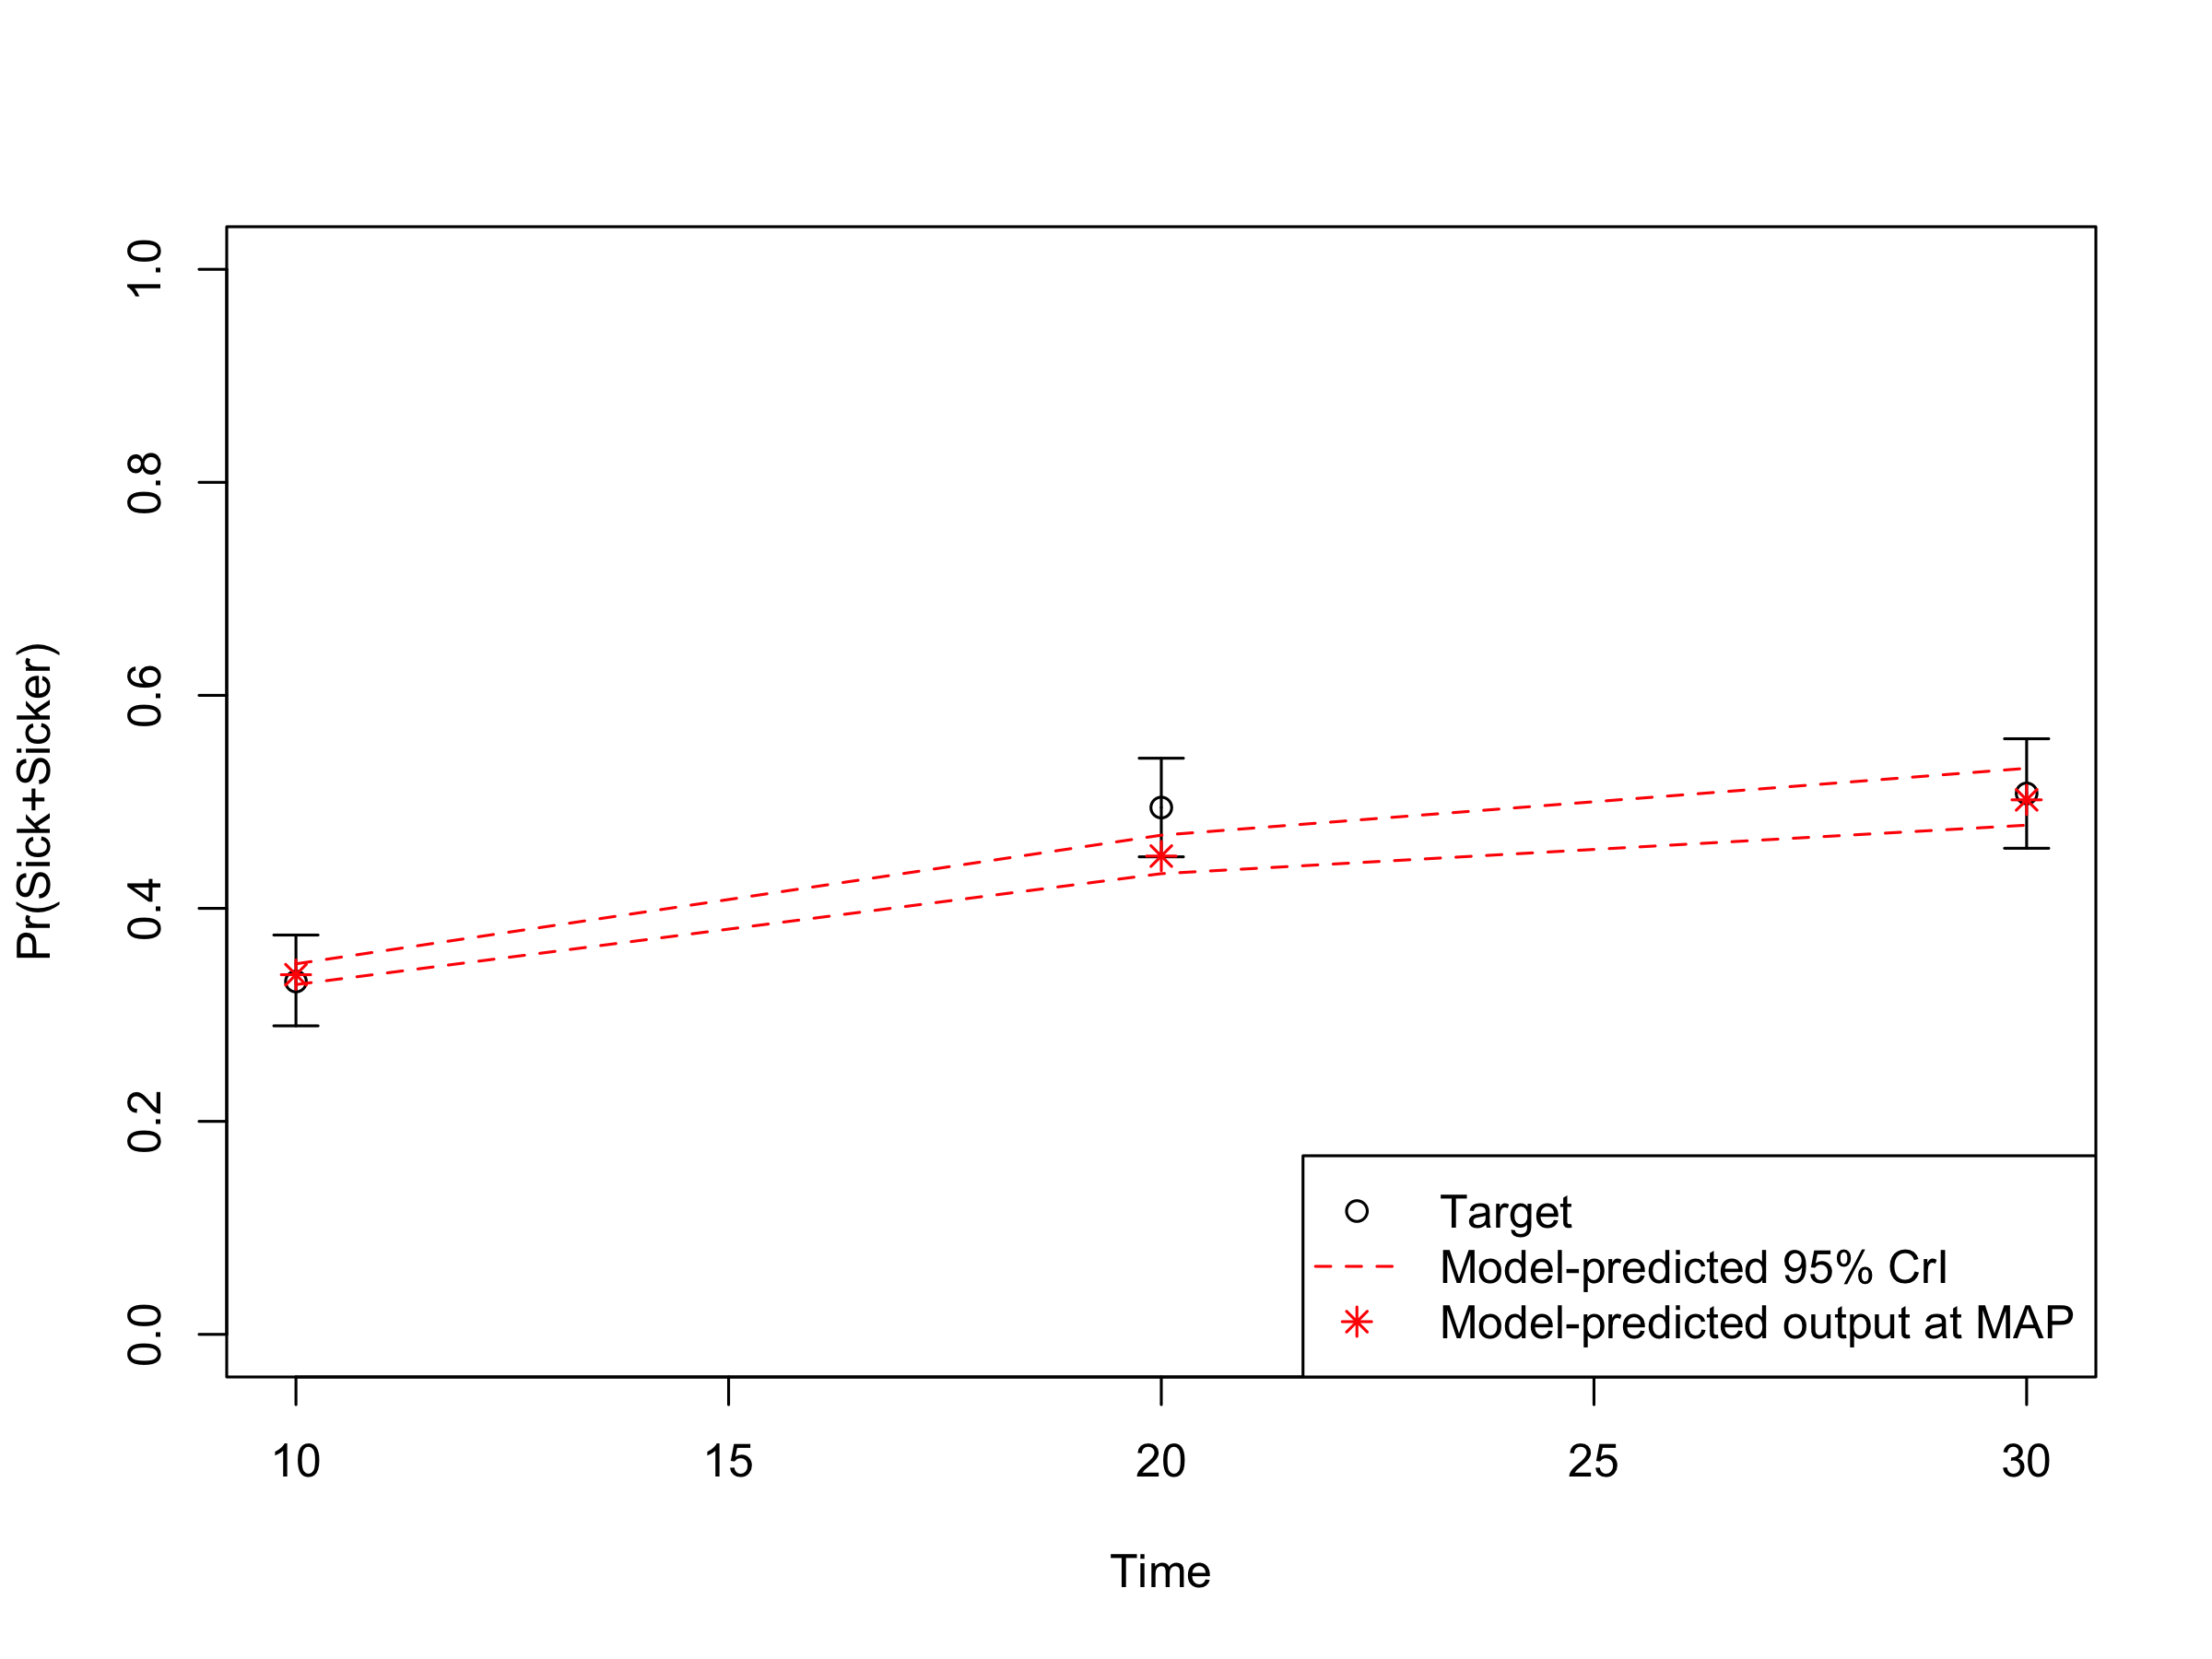
\includegraphics[width=33.33in]{../figs/04_posterior_vs_targets_prevalence} 

}

\caption{Prevalence data of sick individuals: Model-predicted output vs targets.}\label{fig:04-prevalence}
\end{figure}

\begin{figure}

{\centering 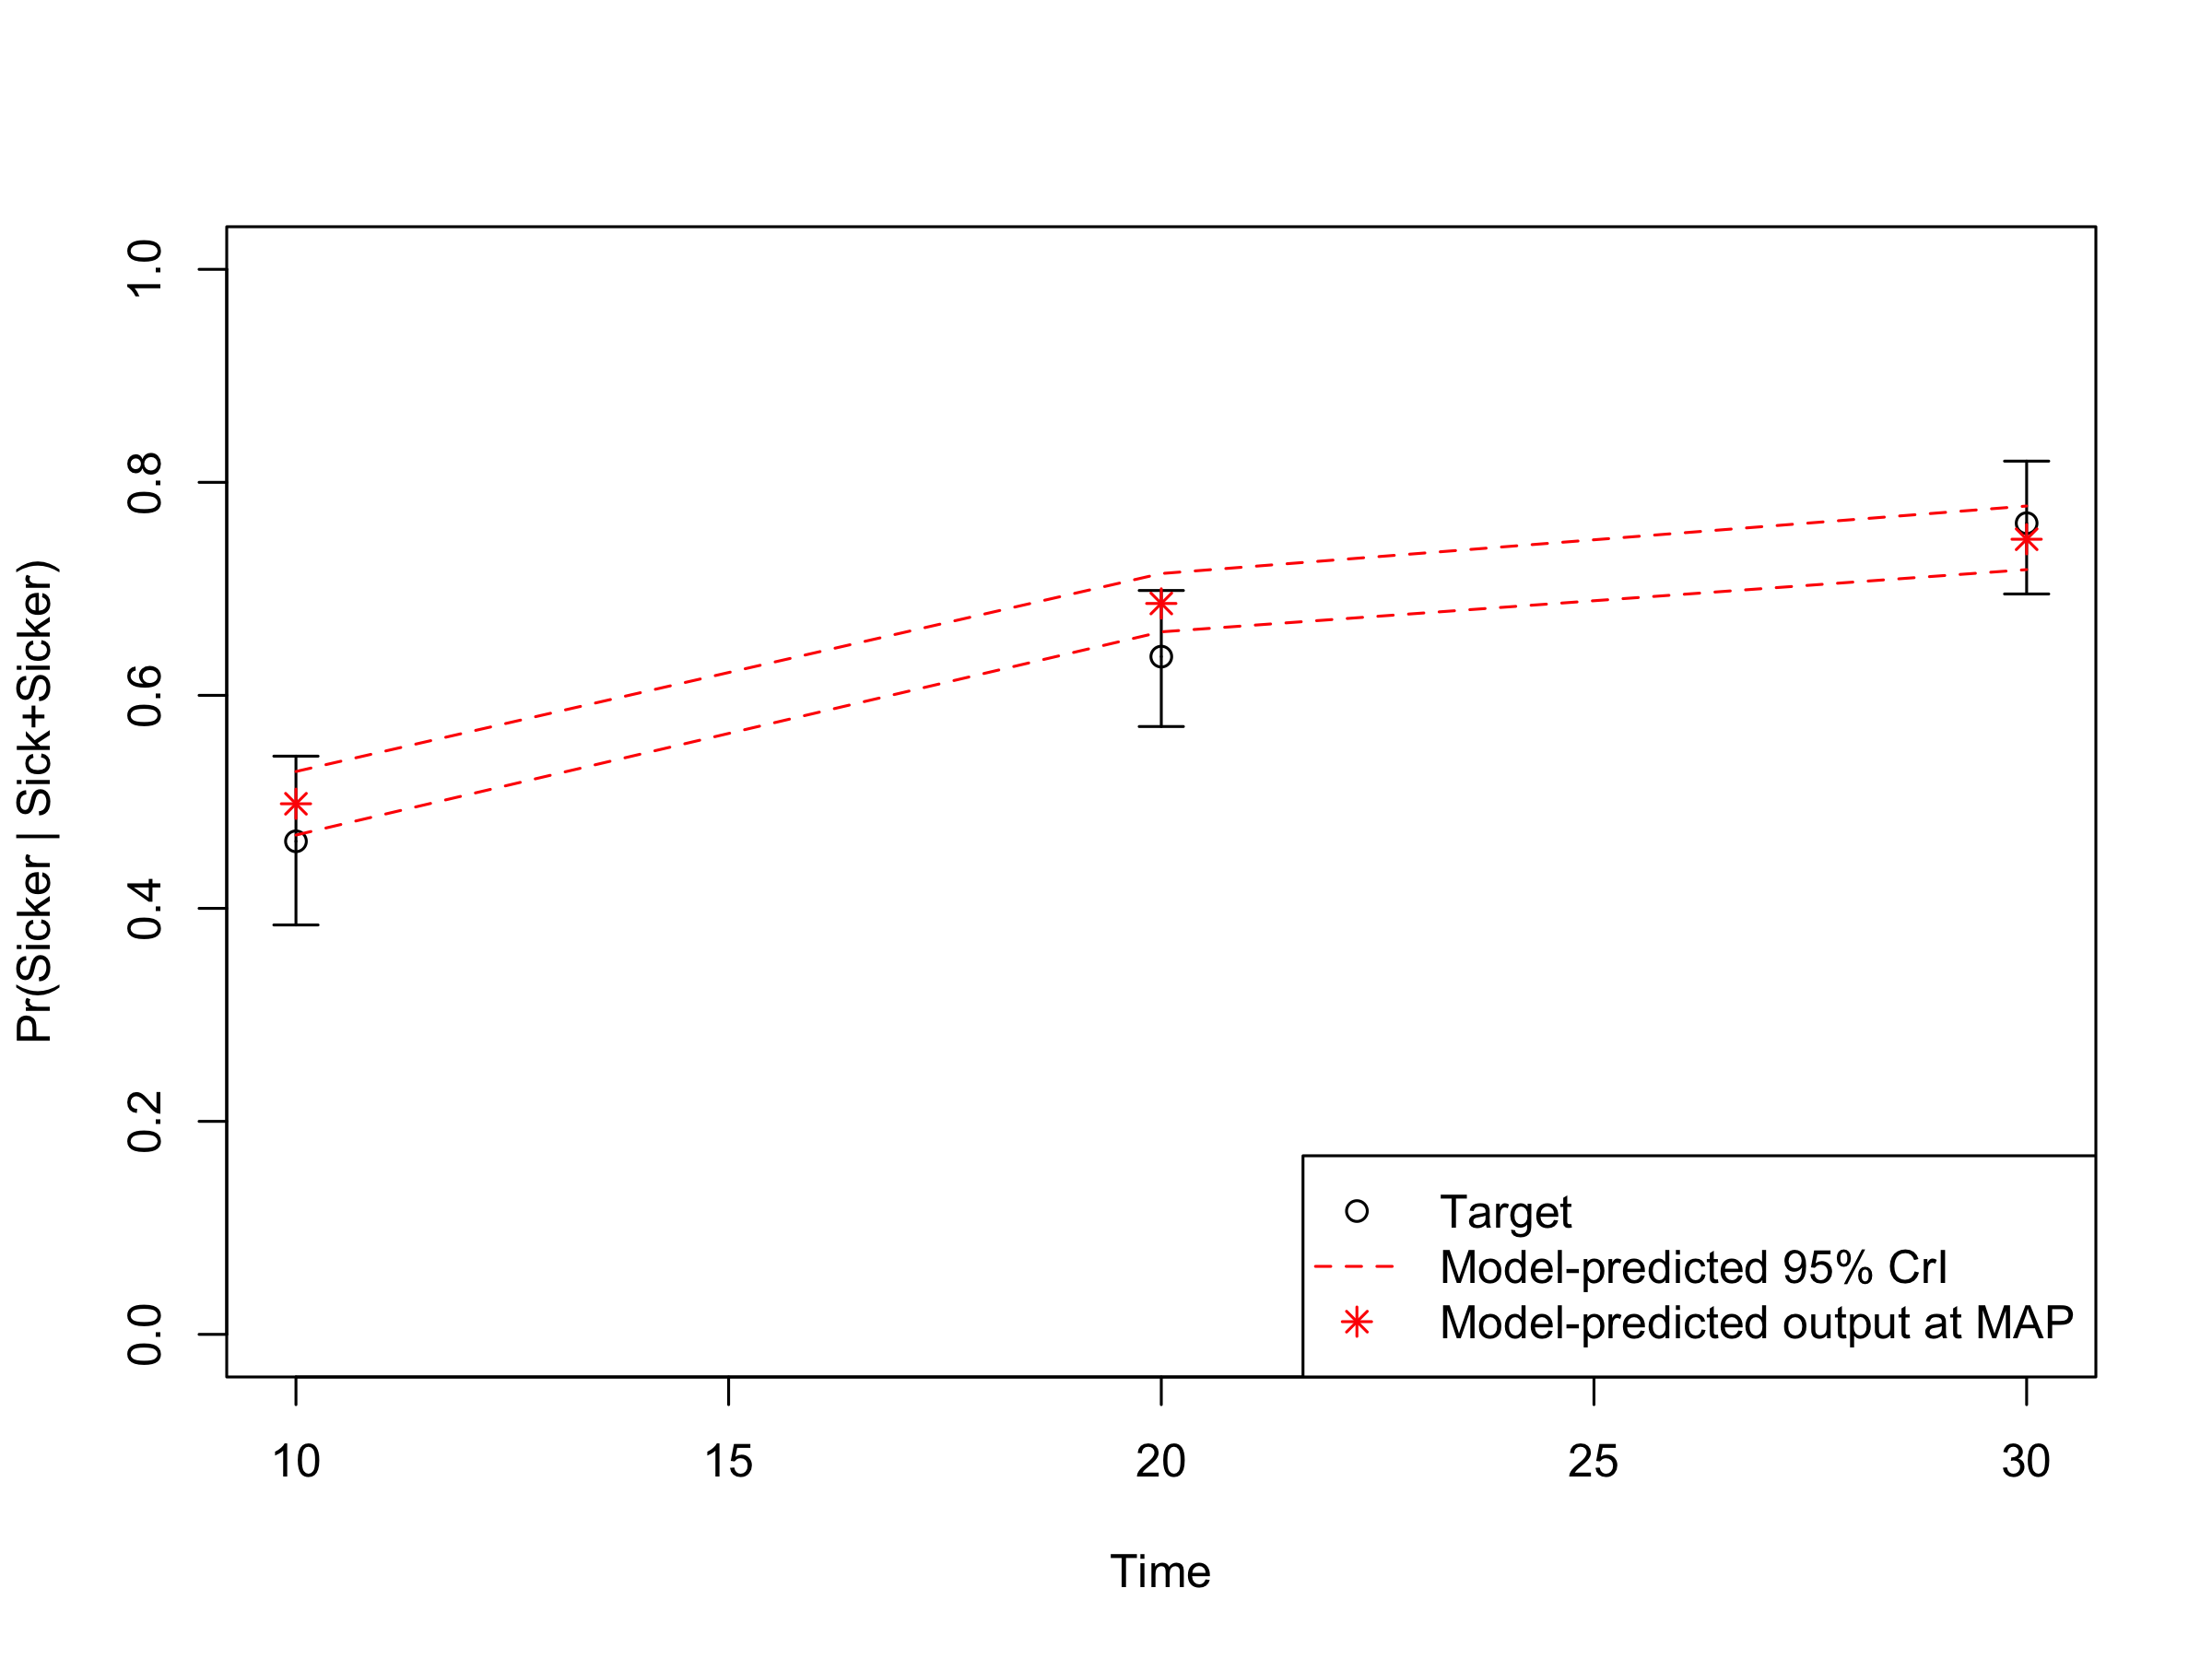
\includegraphics[width=33.33in]{../figs/04_posterior_vs_targets_proportion_sicker} 

}

\caption{Proportion who are Sicker, among all those afflicted (Sick + Sicker): Model-predicted output.}\label{fig:04-proportion}
\end{figure}

\chapter{Analysis}\label{analysis}

The analysis component is where the elements in components 1-4 are
combined to answer the question(s) of interest given current information
and to quantify the value of potential further research. Our framework
separates the analysis in three subcomponents: \emph{05a Deterministic
analysis}, \emph{05b Uncertainty analysis} and \emph{05c Value of
information analysis}. For the Sick-Sicker case-study, we use all three
subcomponents to conduct the CEA and to quantify the uncertainty of our
decision. For procedures in the CEA, we rely on the \texttt{R} package
\texttt{dampack}, which is available here:
\url{https://github.com/DARTH-git/dampack}. Instructions for installing
\texttt{dampack} are described in Appendix 0 provided in the
\emph{app0\_packages\_setup.R} script of the \emph{analysis} folder.

\section{05a Deterministic analysis}\label{Deterministic-analysis}

In this subcomponent, we perform a deterministic CEA, followed by some
deterministic sensitivity analysis, including one-way, two-way and
tornado sensitivity analyses. The function script of this subcomponent,
\emph{05a\_deterministic\_analysis\_function.R}, contains the function
\texttt{calculate\_ce\_out}. This function calculates costs and effects
for a given vector of parameters using a simulation model. We need to
run our simulation model using the calibrated parameter values, but the
list we created in component 01 \ref{inputs} still contain the
placeholder values for the calibrated parameters. This means we need to
update these values by the calibrated values stored in the vector
\texttt{v\_calib\_post\_map}. The function \texttt{update\_param\_list}
updates the list of parameters with new values for some specific
parameters.

\begin{Shaded}
\begin{Highlighting}[]
\KeywordTok{print.function}\NormalTok{(update_param_list)}
\end{Highlighting}
\end{Shaded}

\begin{verbatim}
## function(l_params_all, params_updated){
## 
##   if (typeof(params_updated)!="list"){
##     params_updated <- split(unname(params_updated),names(params_updated)) #converte the named vector to a list
##   }
##   l_params_all <- modifyList(l_params_all, params_updated) #update the values
##   return(l_params_all)
## }
## <bytecode: 0x112beee78>
## <environment: namespace:darthpack>
\end{verbatim}

The first argument of the function, called \texttt{l\_params\_all}, is a
list with all the parameters of decision model. The second argument,
\texttt{params\_updated}, is an object with parameters for which values
need to be updated. The function returns the list
\texttt{l\_params\_all} with updated values.

In the \emph{05a\_deterministic\_analysis.R} script we execute the
\texttt{update\_param\_list} function for our case-study, resulting in
the list \texttt{l\_params\_basecase} where the placeholder values for
\texttt{p\_S1S2}, \texttt{hr\_S1} and \texttt{hr\_S2} are replaced by
the calibration estimates.

\begin{Shaded}
\begin{Highlighting}[]
\NormalTok{l_params_basecase <-}\StringTok{ }\KeywordTok{update_param_list}\NormalTok{(l_params_all, v_calib_post_map) }
\end{Highlighting}
\end{Shaded}

We use this new list as an argument in the \texttt{calculate\_ce\_out}
function. In addition, we specify the willingness-to-pay (WTP) threshold
value using the \texttt{n\_wtp} argument of this function. This WTP
value is used to compute a net monetary benefit (NMB) value. If the user
does not specify the WTP, a default value of \$100,000/QALY will be used
by the function.

\begin{Shaded}
\begin{Highlighting}[]
\NormalTok{df_out_ce <-}\StringTok{ }\KeywordTok{calculate_ce_out}\NormalTok{(}\DataTypeTok{l_params_all =}\NormalTok{ l_params_basecase, }
                                \DataTypeTok{n_wtp =} \DecValTok{150000}\NormalTok{)}
\KeywordTok{print.function}\NormalTok{(calculate_ce_out) }\CommentTok{# print the function}
\end{Highlighting}
\end{Shaded}

\begin{verbatim}
## function(l_params_all = load_all_params(), 
##                              n_wtp = 100000){ # User defined
##   with(as.list(l_params_all), {
##     ## Create discounting vectors
##     v_dwc <- 1 / ((1 + d_e) ^ (0:(n_t))) # vector with discount weights for costs
##     v_dwe <- 1 / ((1 + d_c) ^ (0:(n_t))) # vector with discount weights for QALYs
##     
##     ## Run STM model at a parameter set for each intervention
##     l_model_out_no_trt <- decision_model(l_params_all = l_params_all)
##     l_model_out_trt    <- decision_model(l_params_all = l_params_all)
##     
##     ## Cohort trace by treatment
##     m_M_no_trt <- l_model_out_no_trt$m_M # No treatment
##     m_M_trt    <- l_model_out_trt$m_M    # Treatment
##     
##     ## Vectors with costs and utilities by treatment
##     v_u_no_trt <- c(u_H, u_S1, u_S2, u_D)
##     v_u_trt    <- c(u_H, u_Trt, u_S2, u_D)
##     
##     v_c_no_trt <- c(c_H, c_S1, c_S2, c_D)
##     v_c_trt    <- c(c_H, c_S1 + c_Trt, c_S2 + c_Trt, c_D)
##     
##     ## Mean Costs and QALYs for Treatment and NO Treatment
##     v_tu_no_trt <- m_M_no_trt %*% v_u_no_trt
##     v_tu_trt    <- m_M_trt %*% v_u_trt
##     
##     v_tc_no_trt <- m_M_no_trt %*% v_c_no_trt
##     v_tc_trt    <- m_M_trt %*% v_c_trt
##     
##     ## Total discounted mean Costs and QALYs
##     tu_d_no_trt <- t(v_tu_no_trt) %*% v_dwe 
##     tu_d_trt    <- t(v_tu_trt) %*% v_dwe
##     
##     tc_d_no_trt <- t(v_tc_no_trt) %*% v_dwc
##     tc_d_trt    <- t(v_tc_trt)    %*% v_dwc
##     
##     ## Vector with total discounted mean Costs and QALYs
##     v_tc_d <- c(tc_d_no_trt, tc_d_trt)
##     v_tu_d <- c(tu_d_no_trt, tu_d_trt)
##     
##     ## Vector with discounted net monetary benefits (NMB)
##     v_nmb_d <- v_tu_d * n_wtp - v_tc_d
##     
##     ## Dataframe with discounted costs, effectiveness and NMB
##     df_ce <- data.frame(Strategy = v_names_str,
##                         Cost     = v_tc_d,
##                         Effect   = v_tu_d,
##                         NMB      = v_nmb_d)
##     
##     return(df_ce)
##   }
##   )
## }
## <bytecode: 0x11b382670>
## <environment: namespace:darthpack>
\end{verbatim}

After calculating the discount weights, this function runs the
simulation model using the previously described function
\texttt{decision\_model} in the
\emph{02\_simulatiomn\_model\_function.R} script. Inside the function
\texttt{calculate\_ce\_out}, the simulation model is run for both the
treatment, \texttt{l\_model\_out\_trt}, and no treatment,
\texttt{l\_model\_out\_no\_trt}, strategies of the Sick-Sicker model.
Running it for both treatment strategies is done for illustration
purposes. In this case-study, the resulting cohort traces are identical
and we could have executed it only once.

In the second part of the function we create multiple vectors for both
the cost and effects of both strategies. These vectors multiply the
cohort trace to compute the cycle-specific rewards. This results in
vectors of total costs (\texttt{v\_tc}) and total effects
(\texttt{v\_tu}) per cycle. By multiplying these vectors with the
vectors with the discount weights for costs (\texttt{v\_dwc}) and
effects (\texttt{v\_dwe}) we get the total discounted mean costs
(\texttt{tc\_d\_no\_trt} and \texttt{tc\_d\_trt}) and QALYs
(\texttt{tu\_d\_no\_trt} and \texttt{tu\_d\_trt}) for both strategies.
These values are used in the calculation of the NMB. Finally, the total
discounted costs, effectiveness and NMB are combined in the dataframe
\texttt{df\_ce}. The results for our case-study are shown below.

\begin{Shaded}
\begin{Highlighting}[]
\NormalTok{df_out_ce }\CommentTok{# print the dataframe }
\end{Highlighting}
\end{Shaded}

\begin{verbatim}
##       Strategy     Cost   Effect     NMB
## 1 No Treatment 115239.8 20.02366 2888309
## 2    Treatment 214157.6 20.72299 2894291
\end{verbatim}

This dataframe of CE results can be used as an argument in the
\texttt{calculate\_icers} function from the \texttt{dampack} package to
calculate the incremental cost-effectiveness ratios (ICERs) and noting
which strategies are weakly and strongly dominated. Table
\ref{tab:df-cea-det} shows the result of the deterministic CEA.

\begin{Shaded}
\begin{Highlighting}[]
\NormalTok{df_cea_det <-}\StringTok{ }\KeywordTok{calculate_icers}\NormalTok{(}\DataTypeTok{cost =}\NormalTok{ df_out_ce}\OperatorTok{$}\NormalTok{Cost, }
                              \DataTypeTok{effect =}\NormalTok{ df_out_ce}\OperatorTok{$}\NormalTok{Effect, }
                              \DataTypeTok{strategies =}\NormalTok{ l_params_basecase}\OperatorTok{$}\NormalTok{v_names_str)}
\end{Highlighting}
\end{Shaded}

\begin{table}[t]

\caption{\label{tab:df-cea-det}Deterministic cost-effectiveness analysis results of the Sick-Sicker model comparing no treatment with treatment.}
\centering
\begin{tabular}{l|r|r|r|r|r}
\hline
Strategy & Cost & Effect & Inc\_Cost & Inc\_Effect & ICER\\
\hline
No Treatment & 115239.8 & 20.02366 & NA & NA & NA\\
\hline
Treatment & 214157.6 & 20.72299 & 98917.83 & 0.6993333 & 141445.9\\
\hline
\end{tabular}
\end{table}

Finally, Figure \ref{fig:05a-CEA-frontier} shows the cost-effectiveness
frontier of the CEA.

\begin{figure}

{\centering 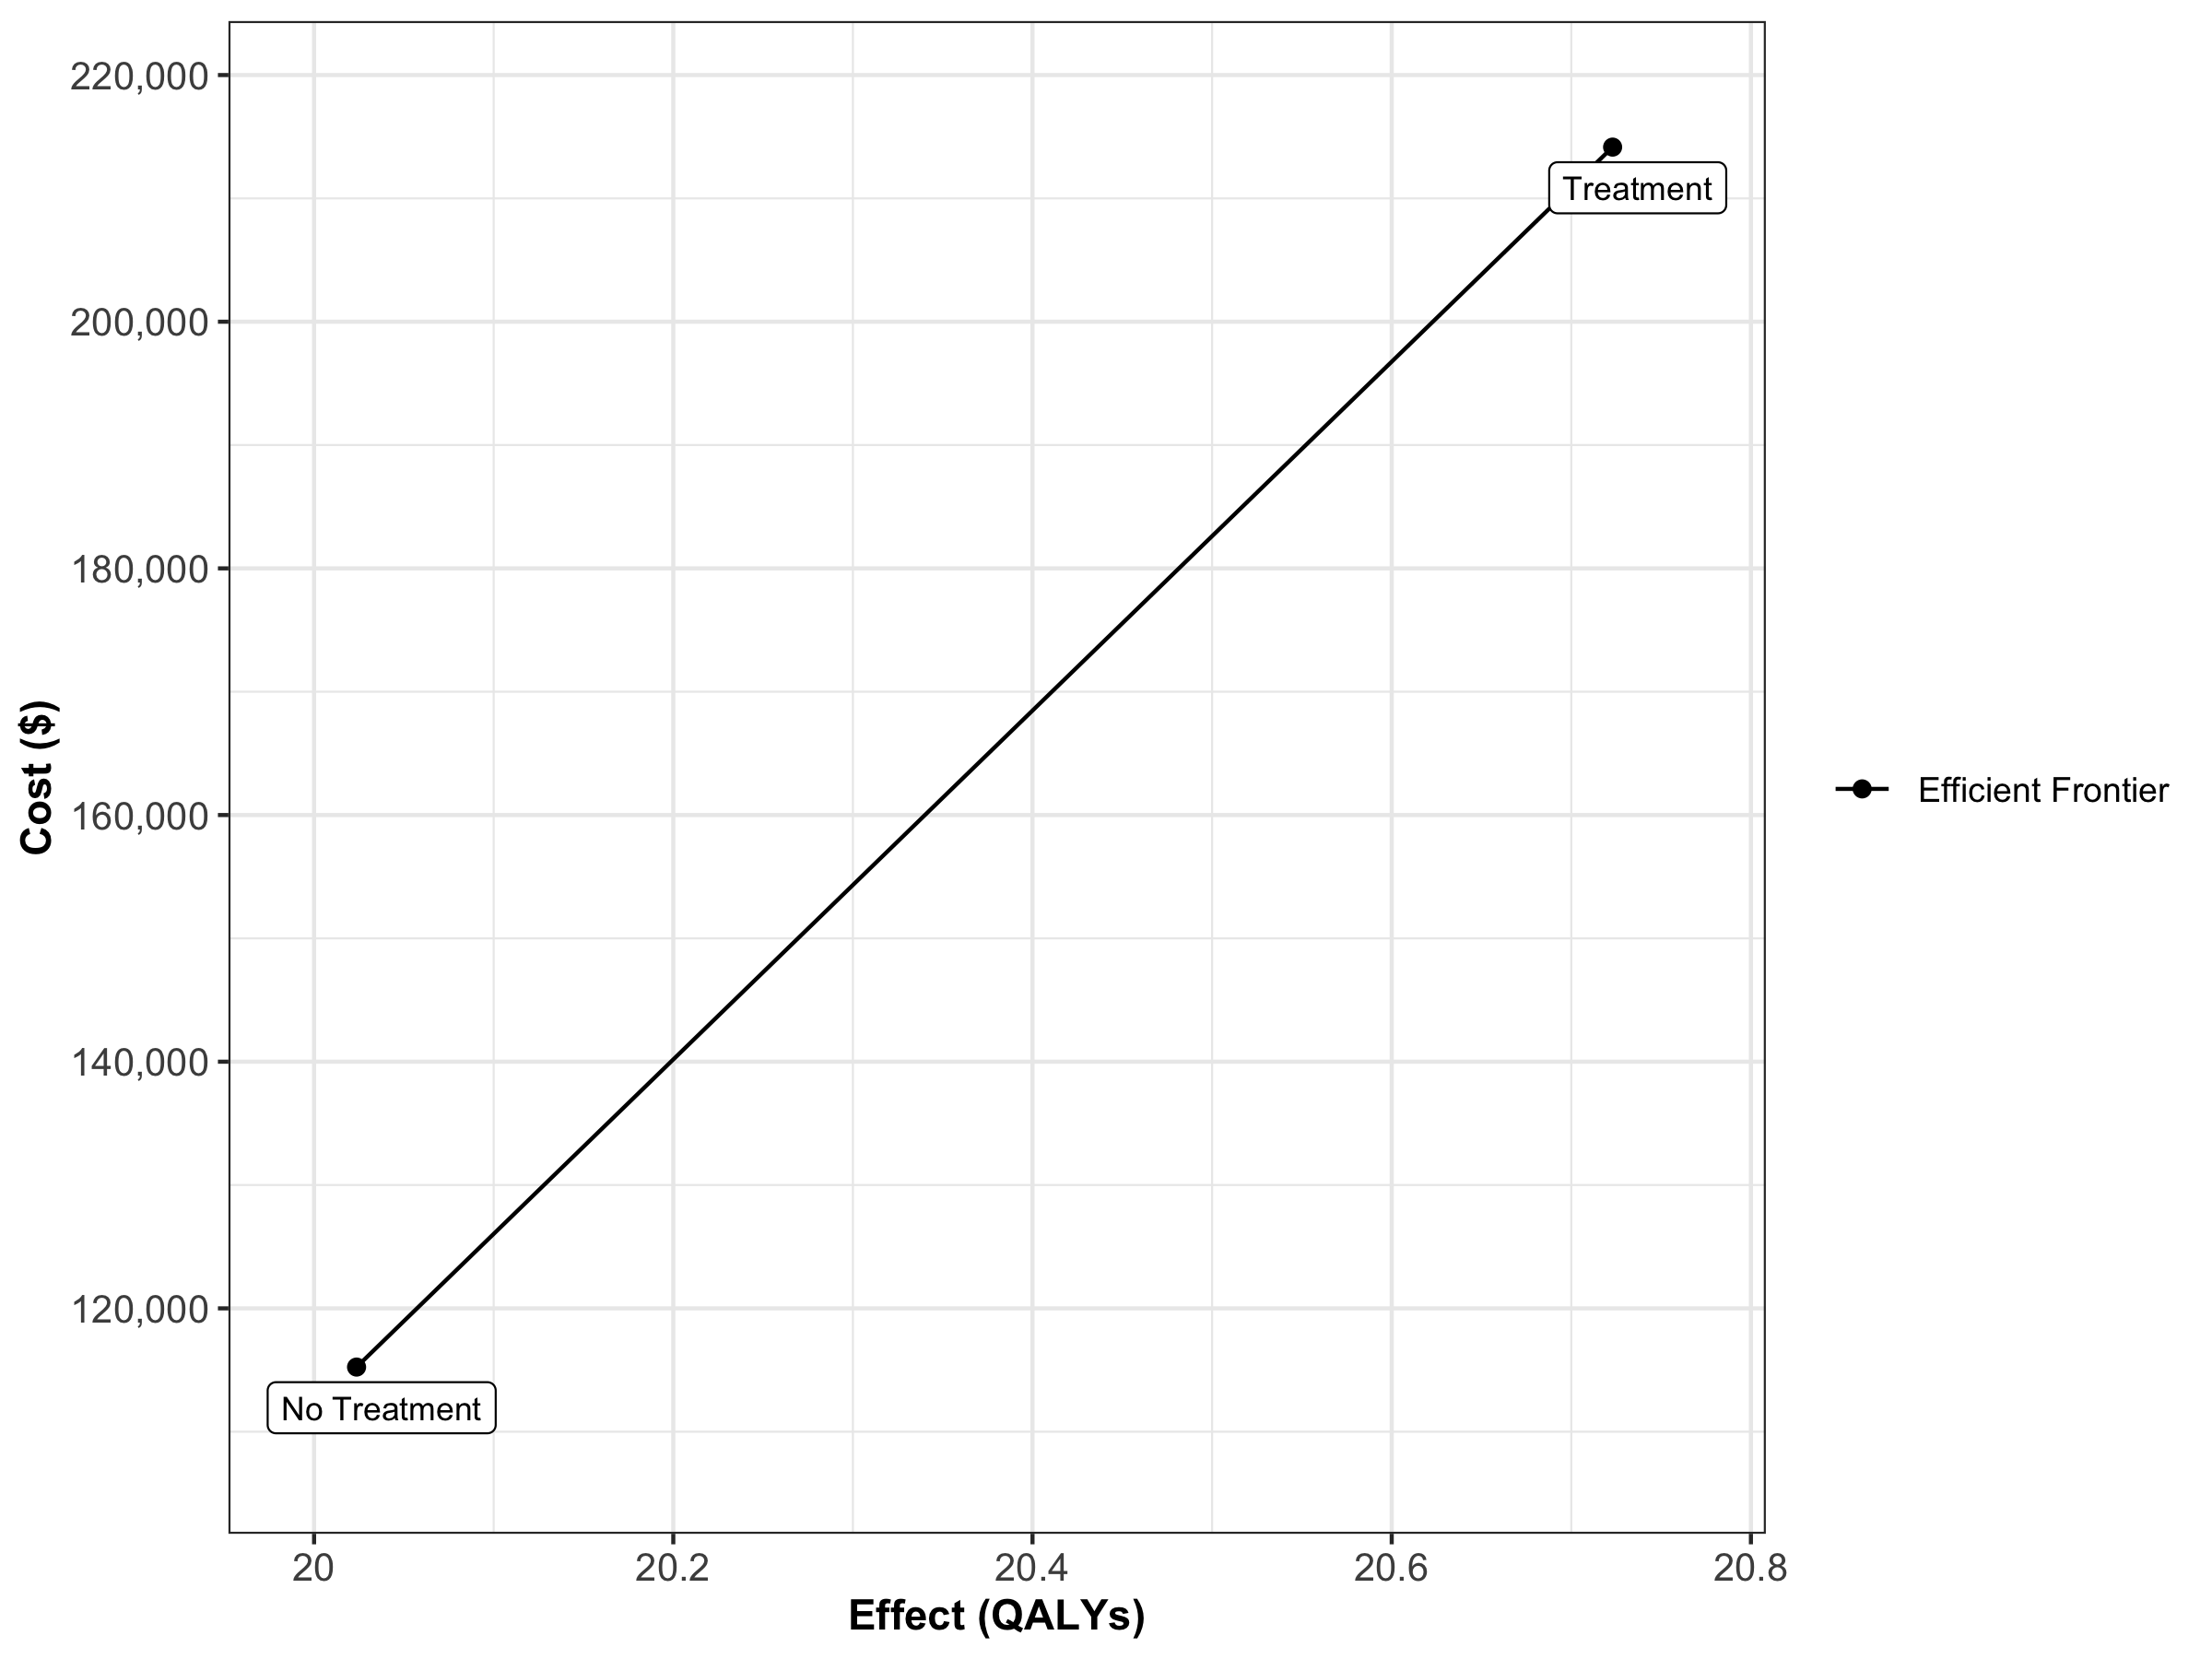
\includegraphics[width=33.33in]{../figs/05a_cea_frontier} 

}

\caption{Cost-effectiveness frontier.}\label{fig:05a-CEA-frontier}
\end{figure}

We then conduct a series of deterministic sensitivity analysis. First,
we conduct a one-way sensitivity analysis (OWSA) on the variables
\texttt{c\_Trt}, \texttt{p\_HS1}, \texttt{u\_S1} and \texttt{u\_Trt} and
a two-way sensitivity analysis (TWSA) using the owsa\_det and twsa\_det
functions. We use the output of these functions to produce different SA
plots, such as OWSA tornado, one-way optimal strategy and TWSA plots
(Figures \ref{fig:05a-owsa-nmb} - \ref{fig:05a-twsa-uS1-uTrt-nmb}).

\begin{figure}

{\centering 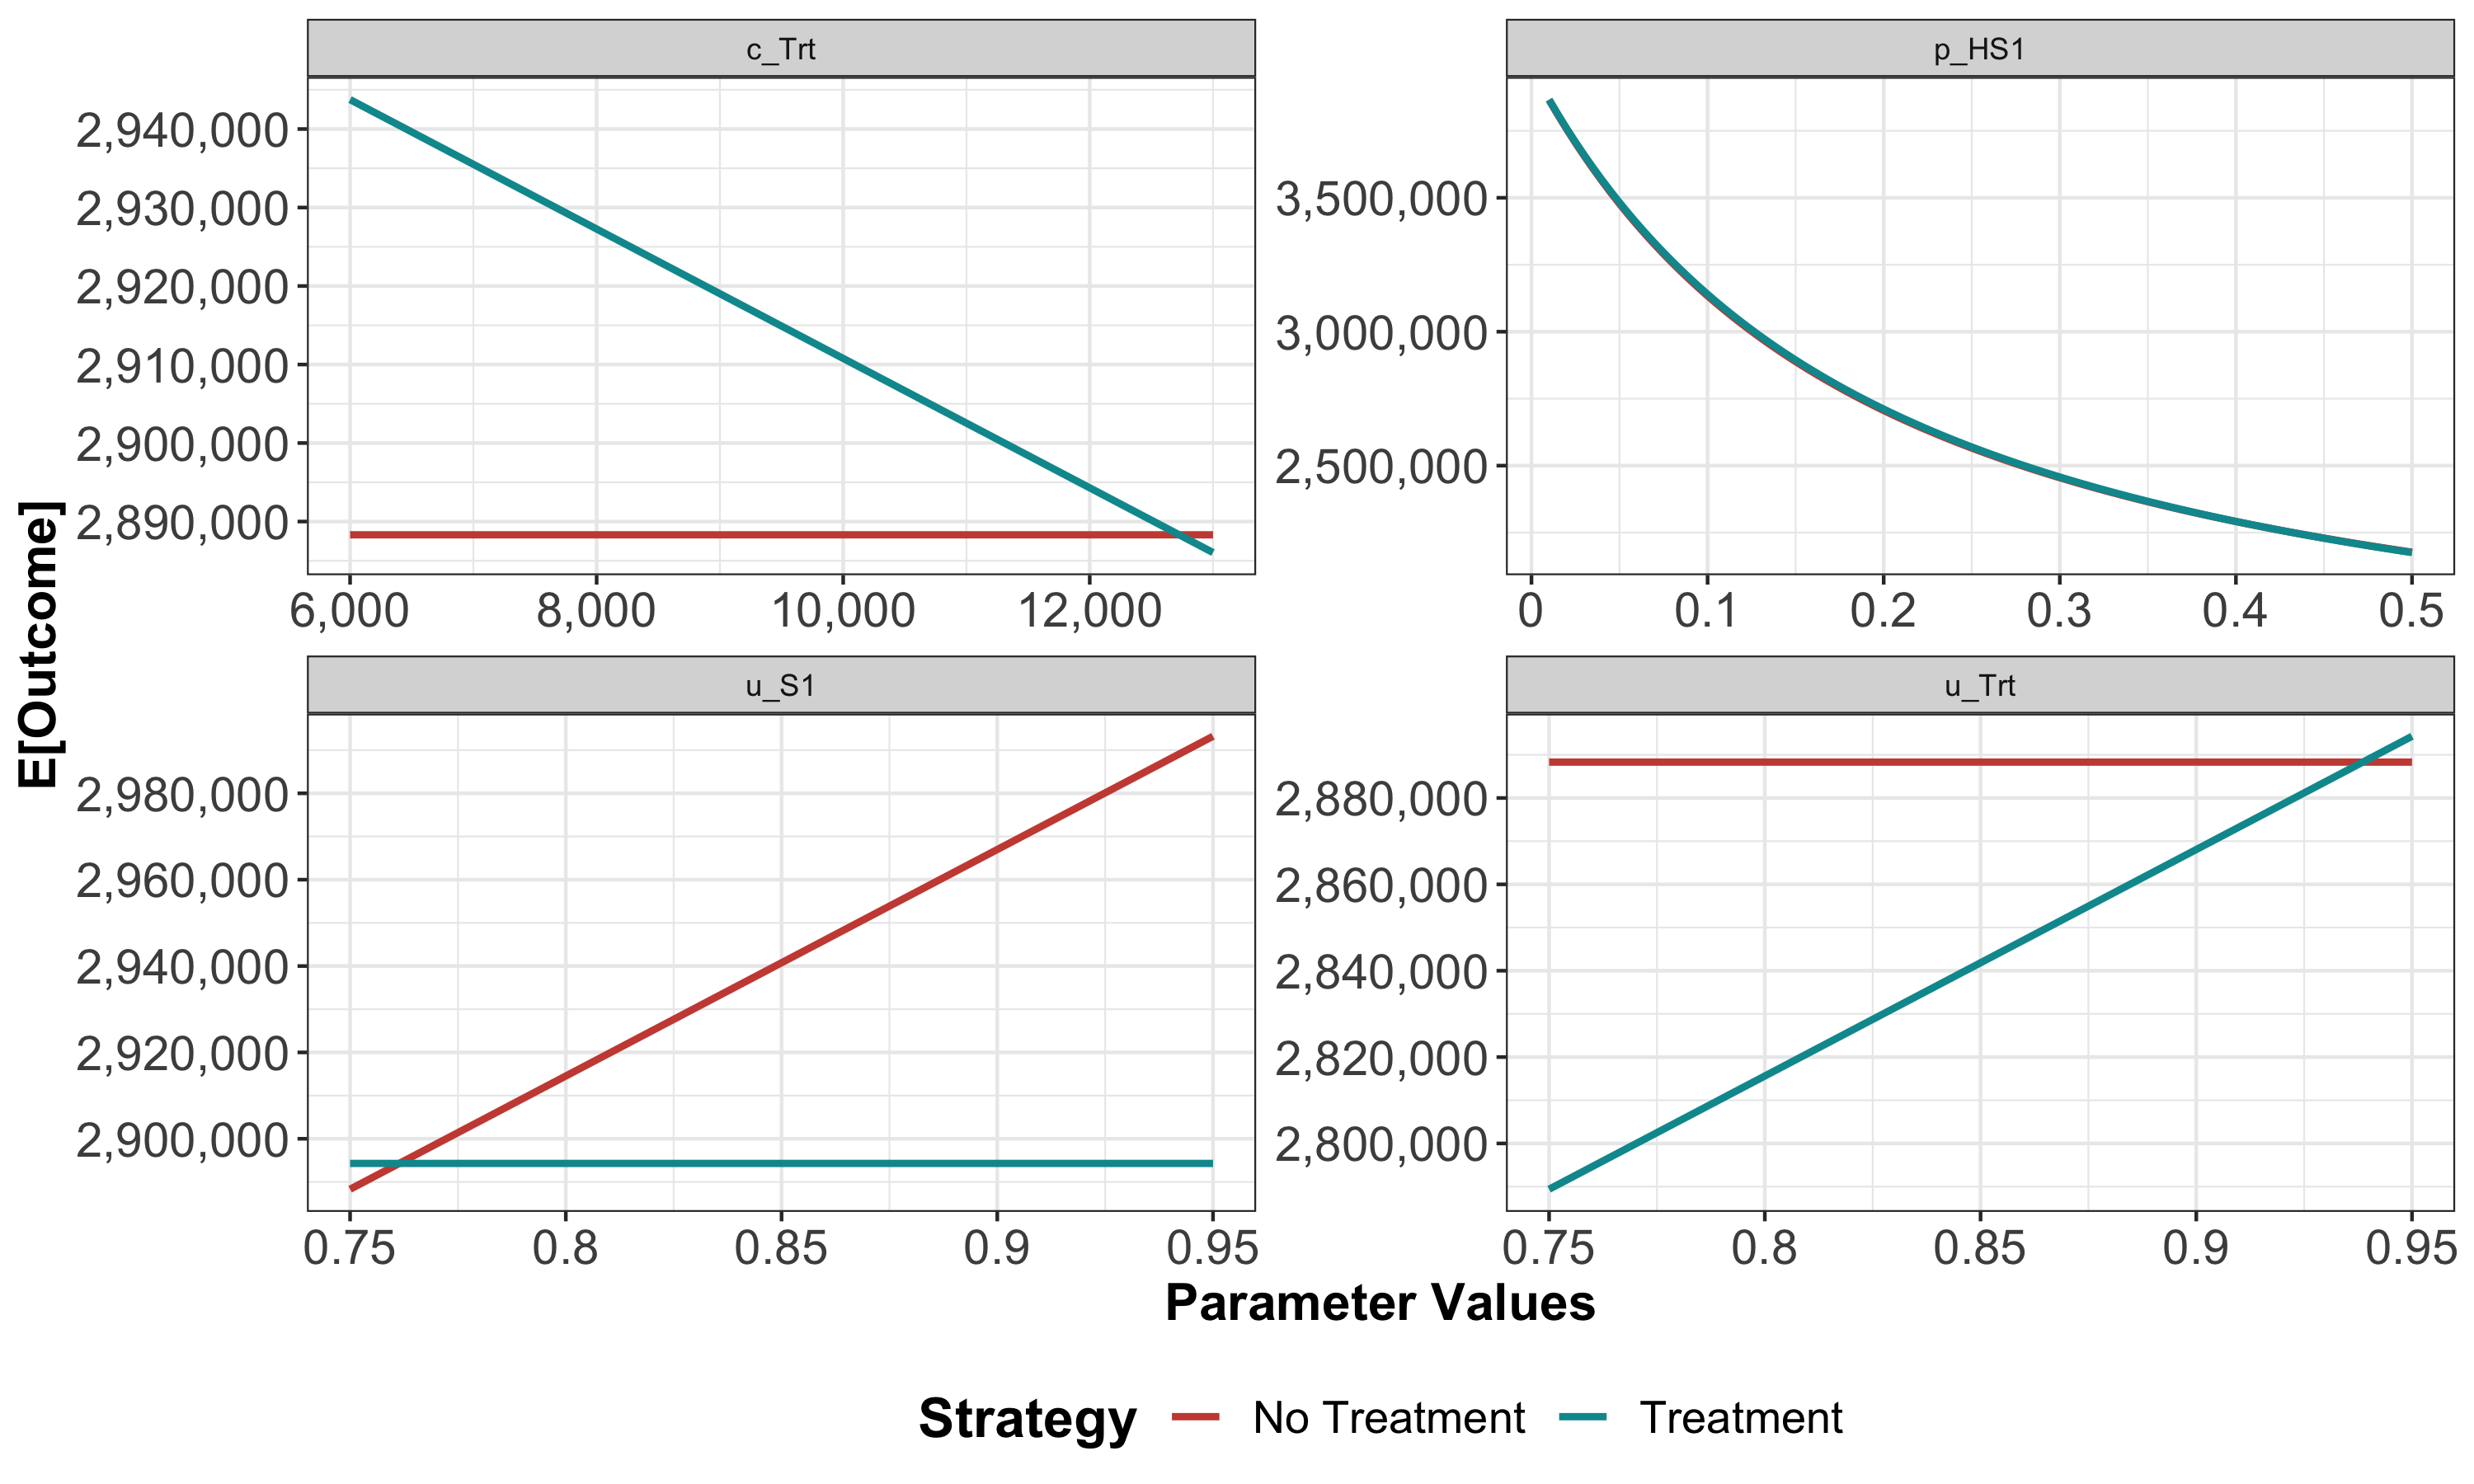
\includegraphics[width=41.67in]{../figs/05a_owsa_nmb} 

}

\caption{One-way sensitivity analysis results}\label{fig:05a-owsa-nmb}
\end{figure}

\begin{figure}

{\centering 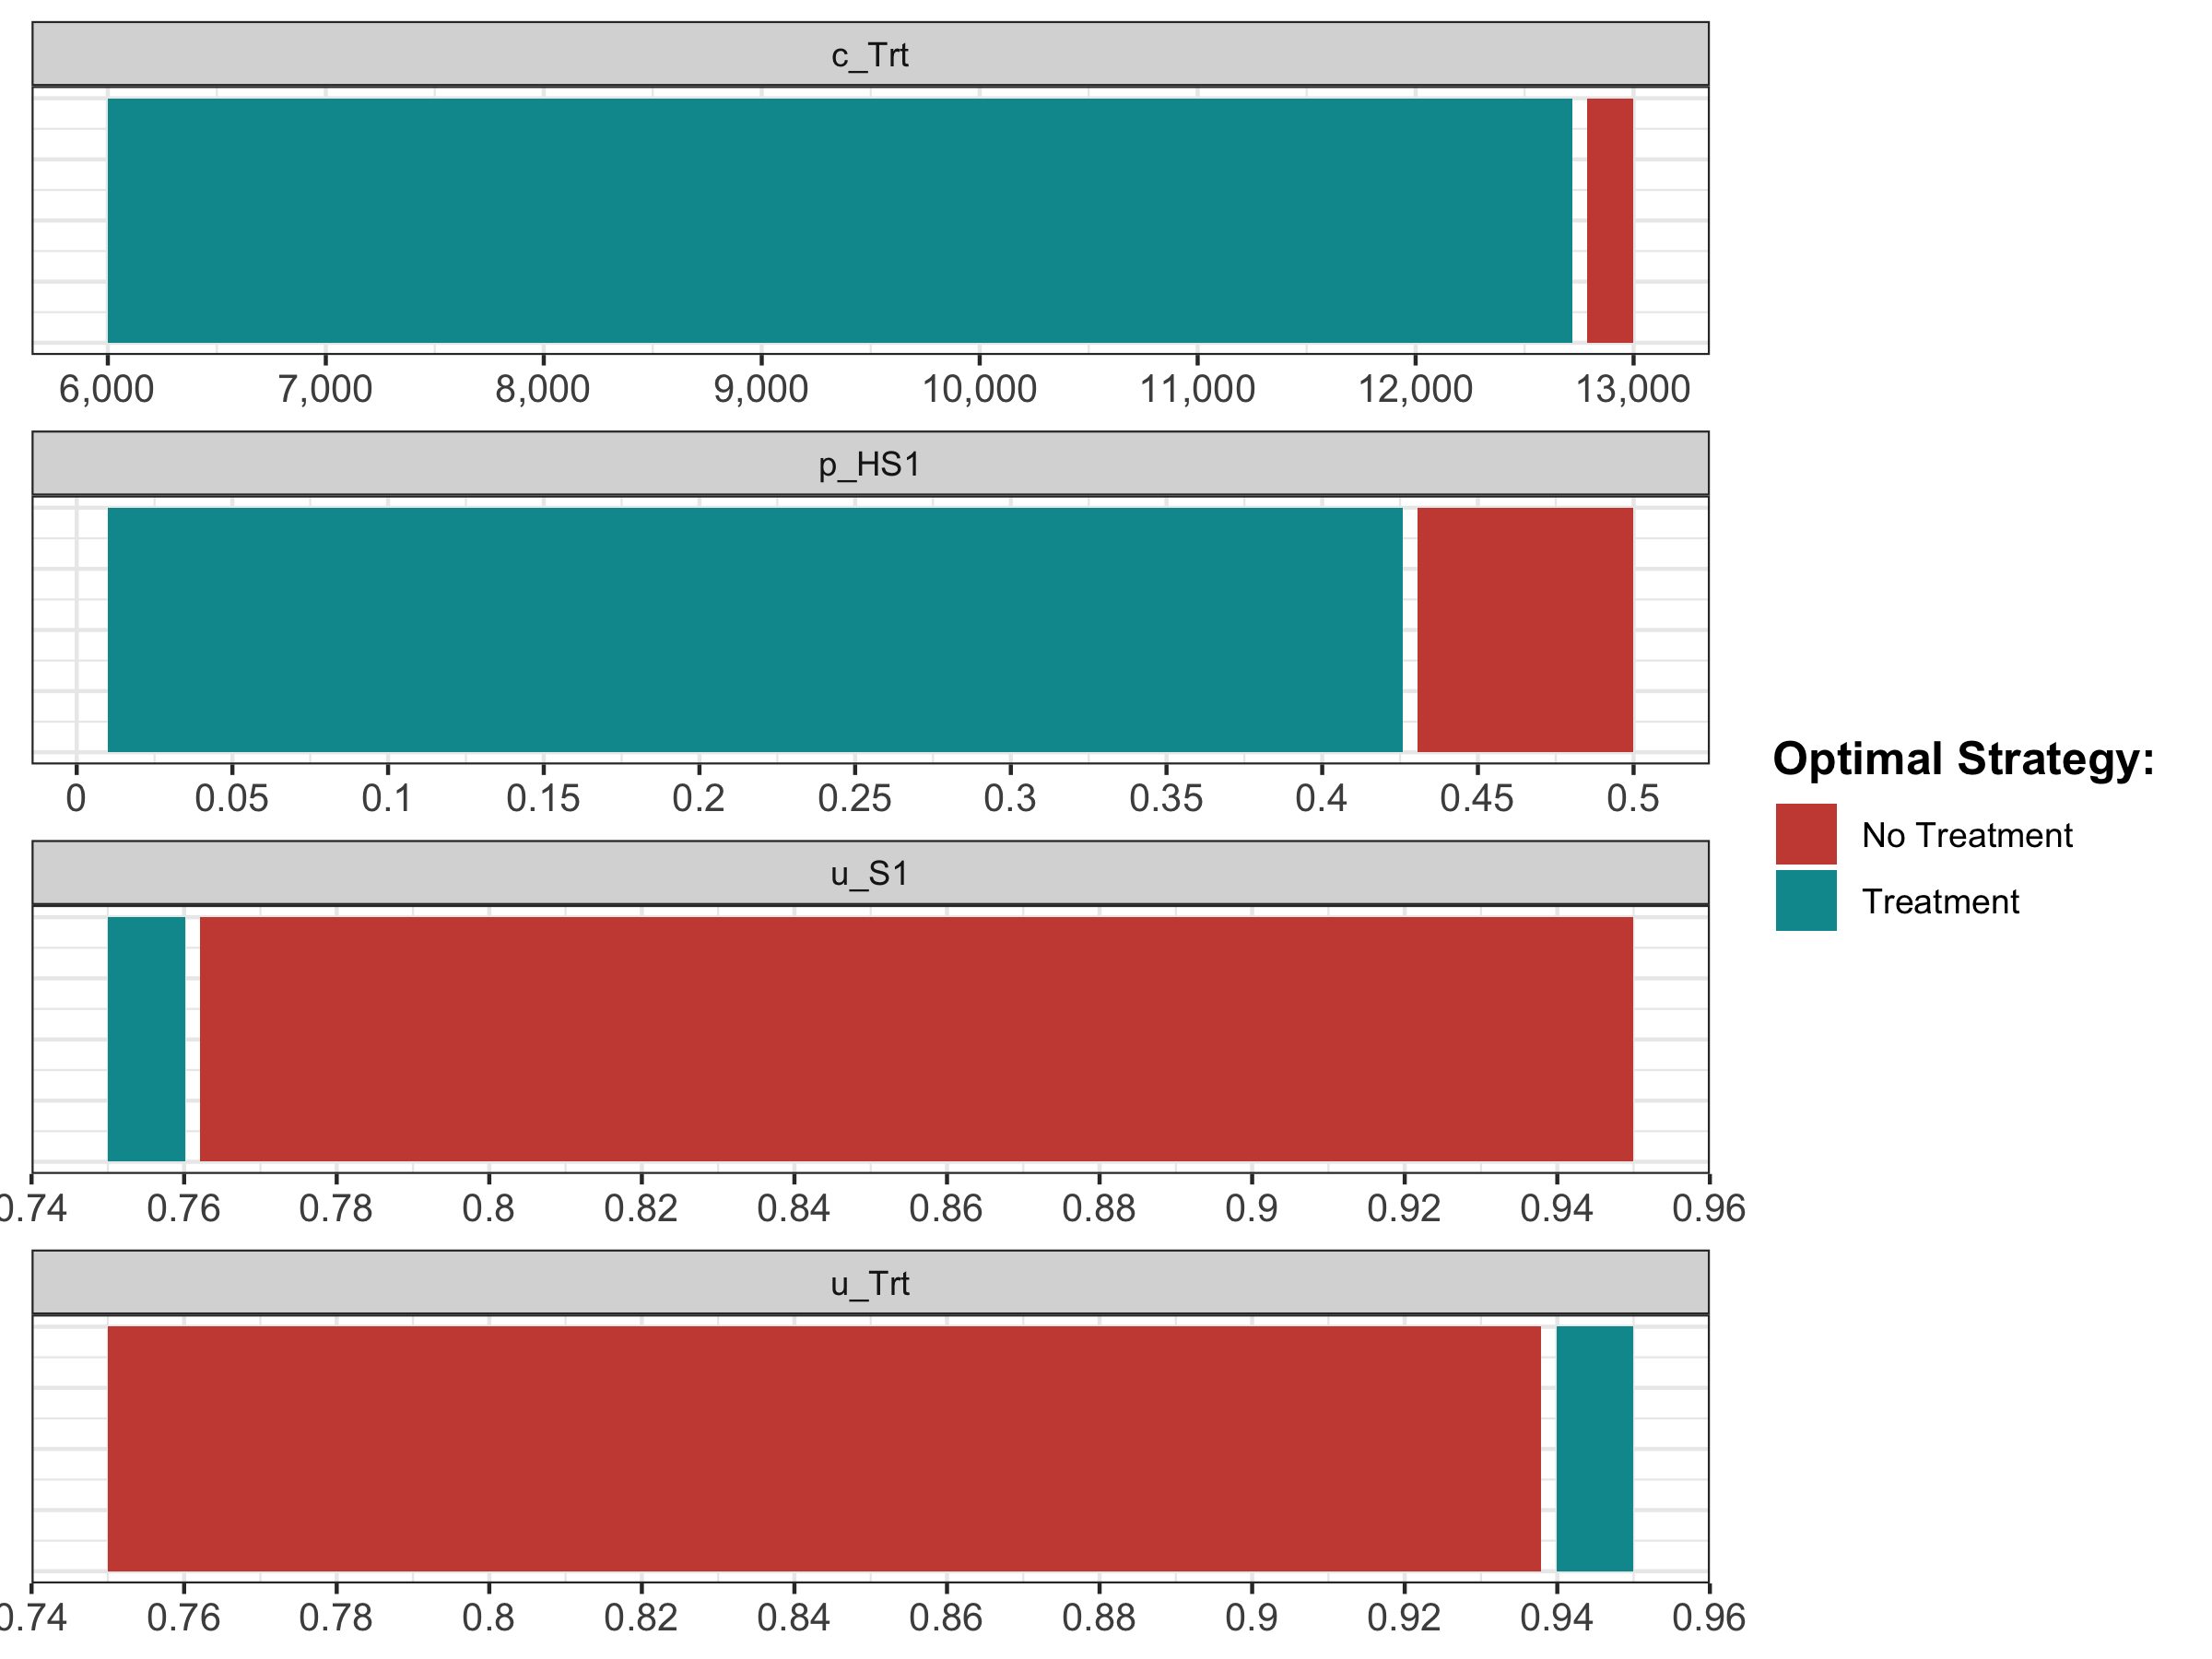
\includegraphics[width=33.33in]{../figs/05a_optimal_owsa_nmb} 

}

\caption{The optimal strategy with OWSA}\label{fig:05a-optimal-owsa-nmb}
\end{figure}

\begin{figure}

{\centering 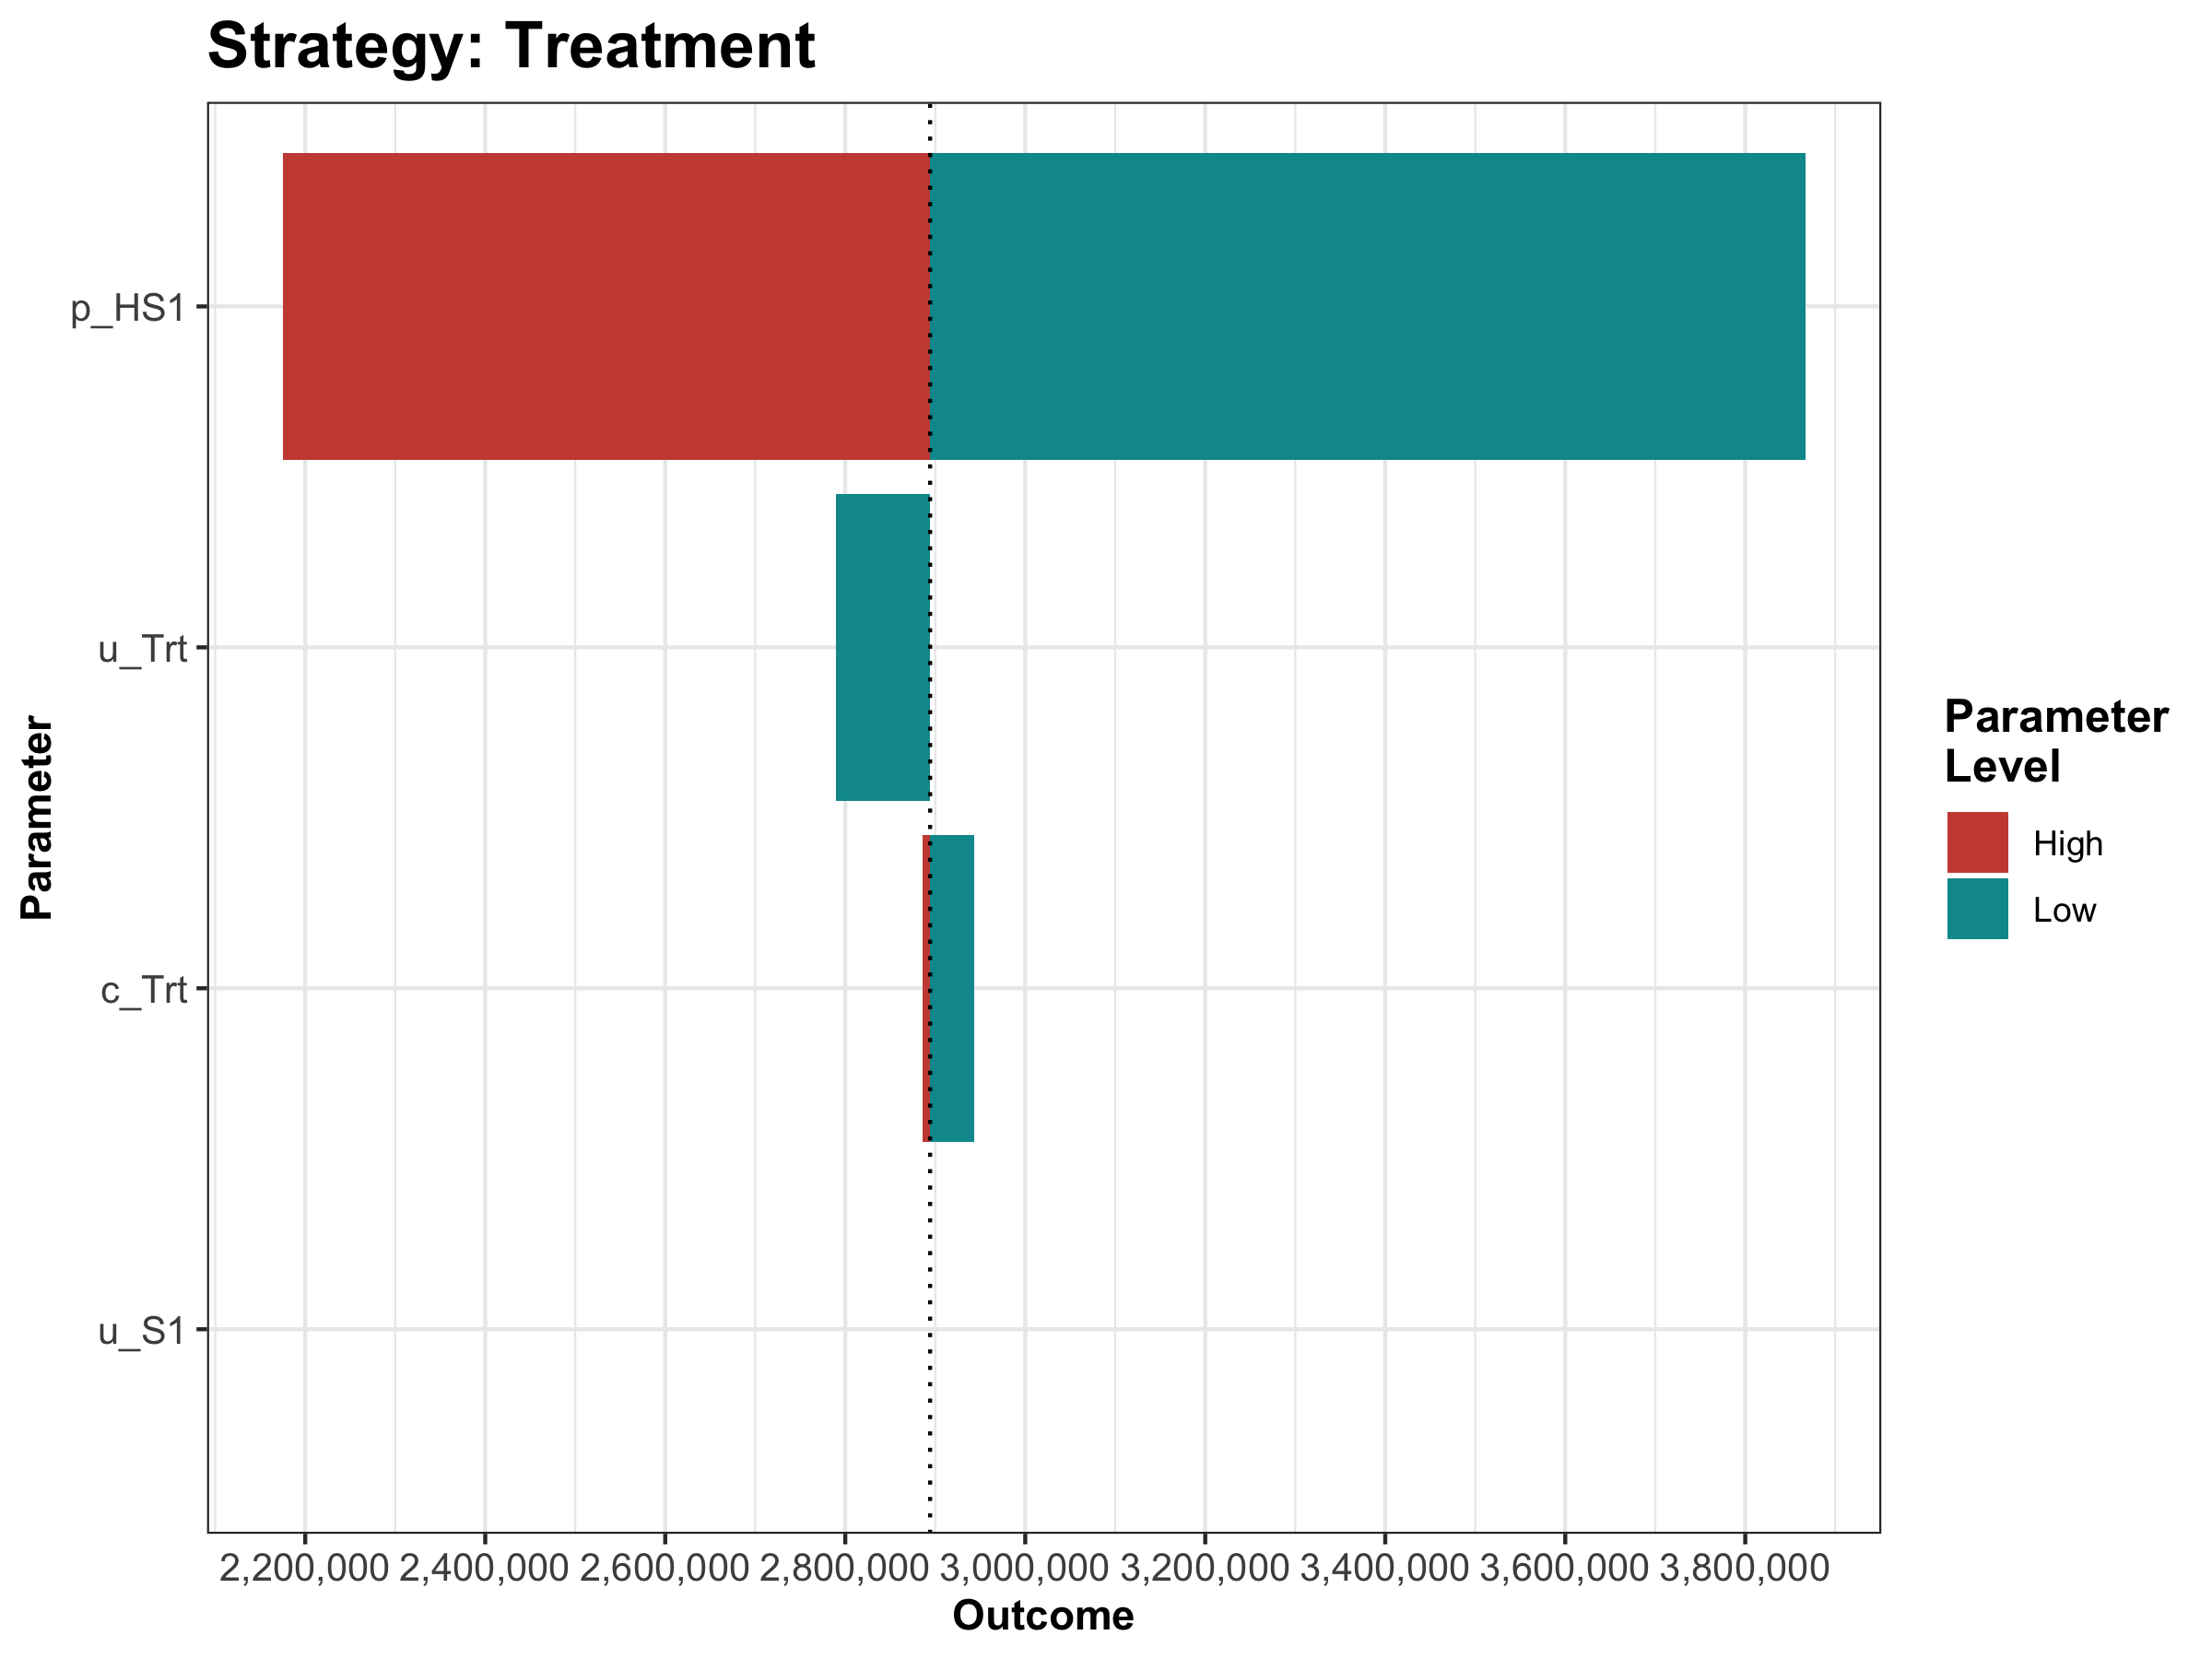
\includegraphics[width=33.33in]{../figs/05a_tornado_Treatment_nmb} 

}

\caption{The tornado plot}\label{fig:05a-tornado-Treatment-nmb}
\end{figure}

\begin{figure}

{\centering 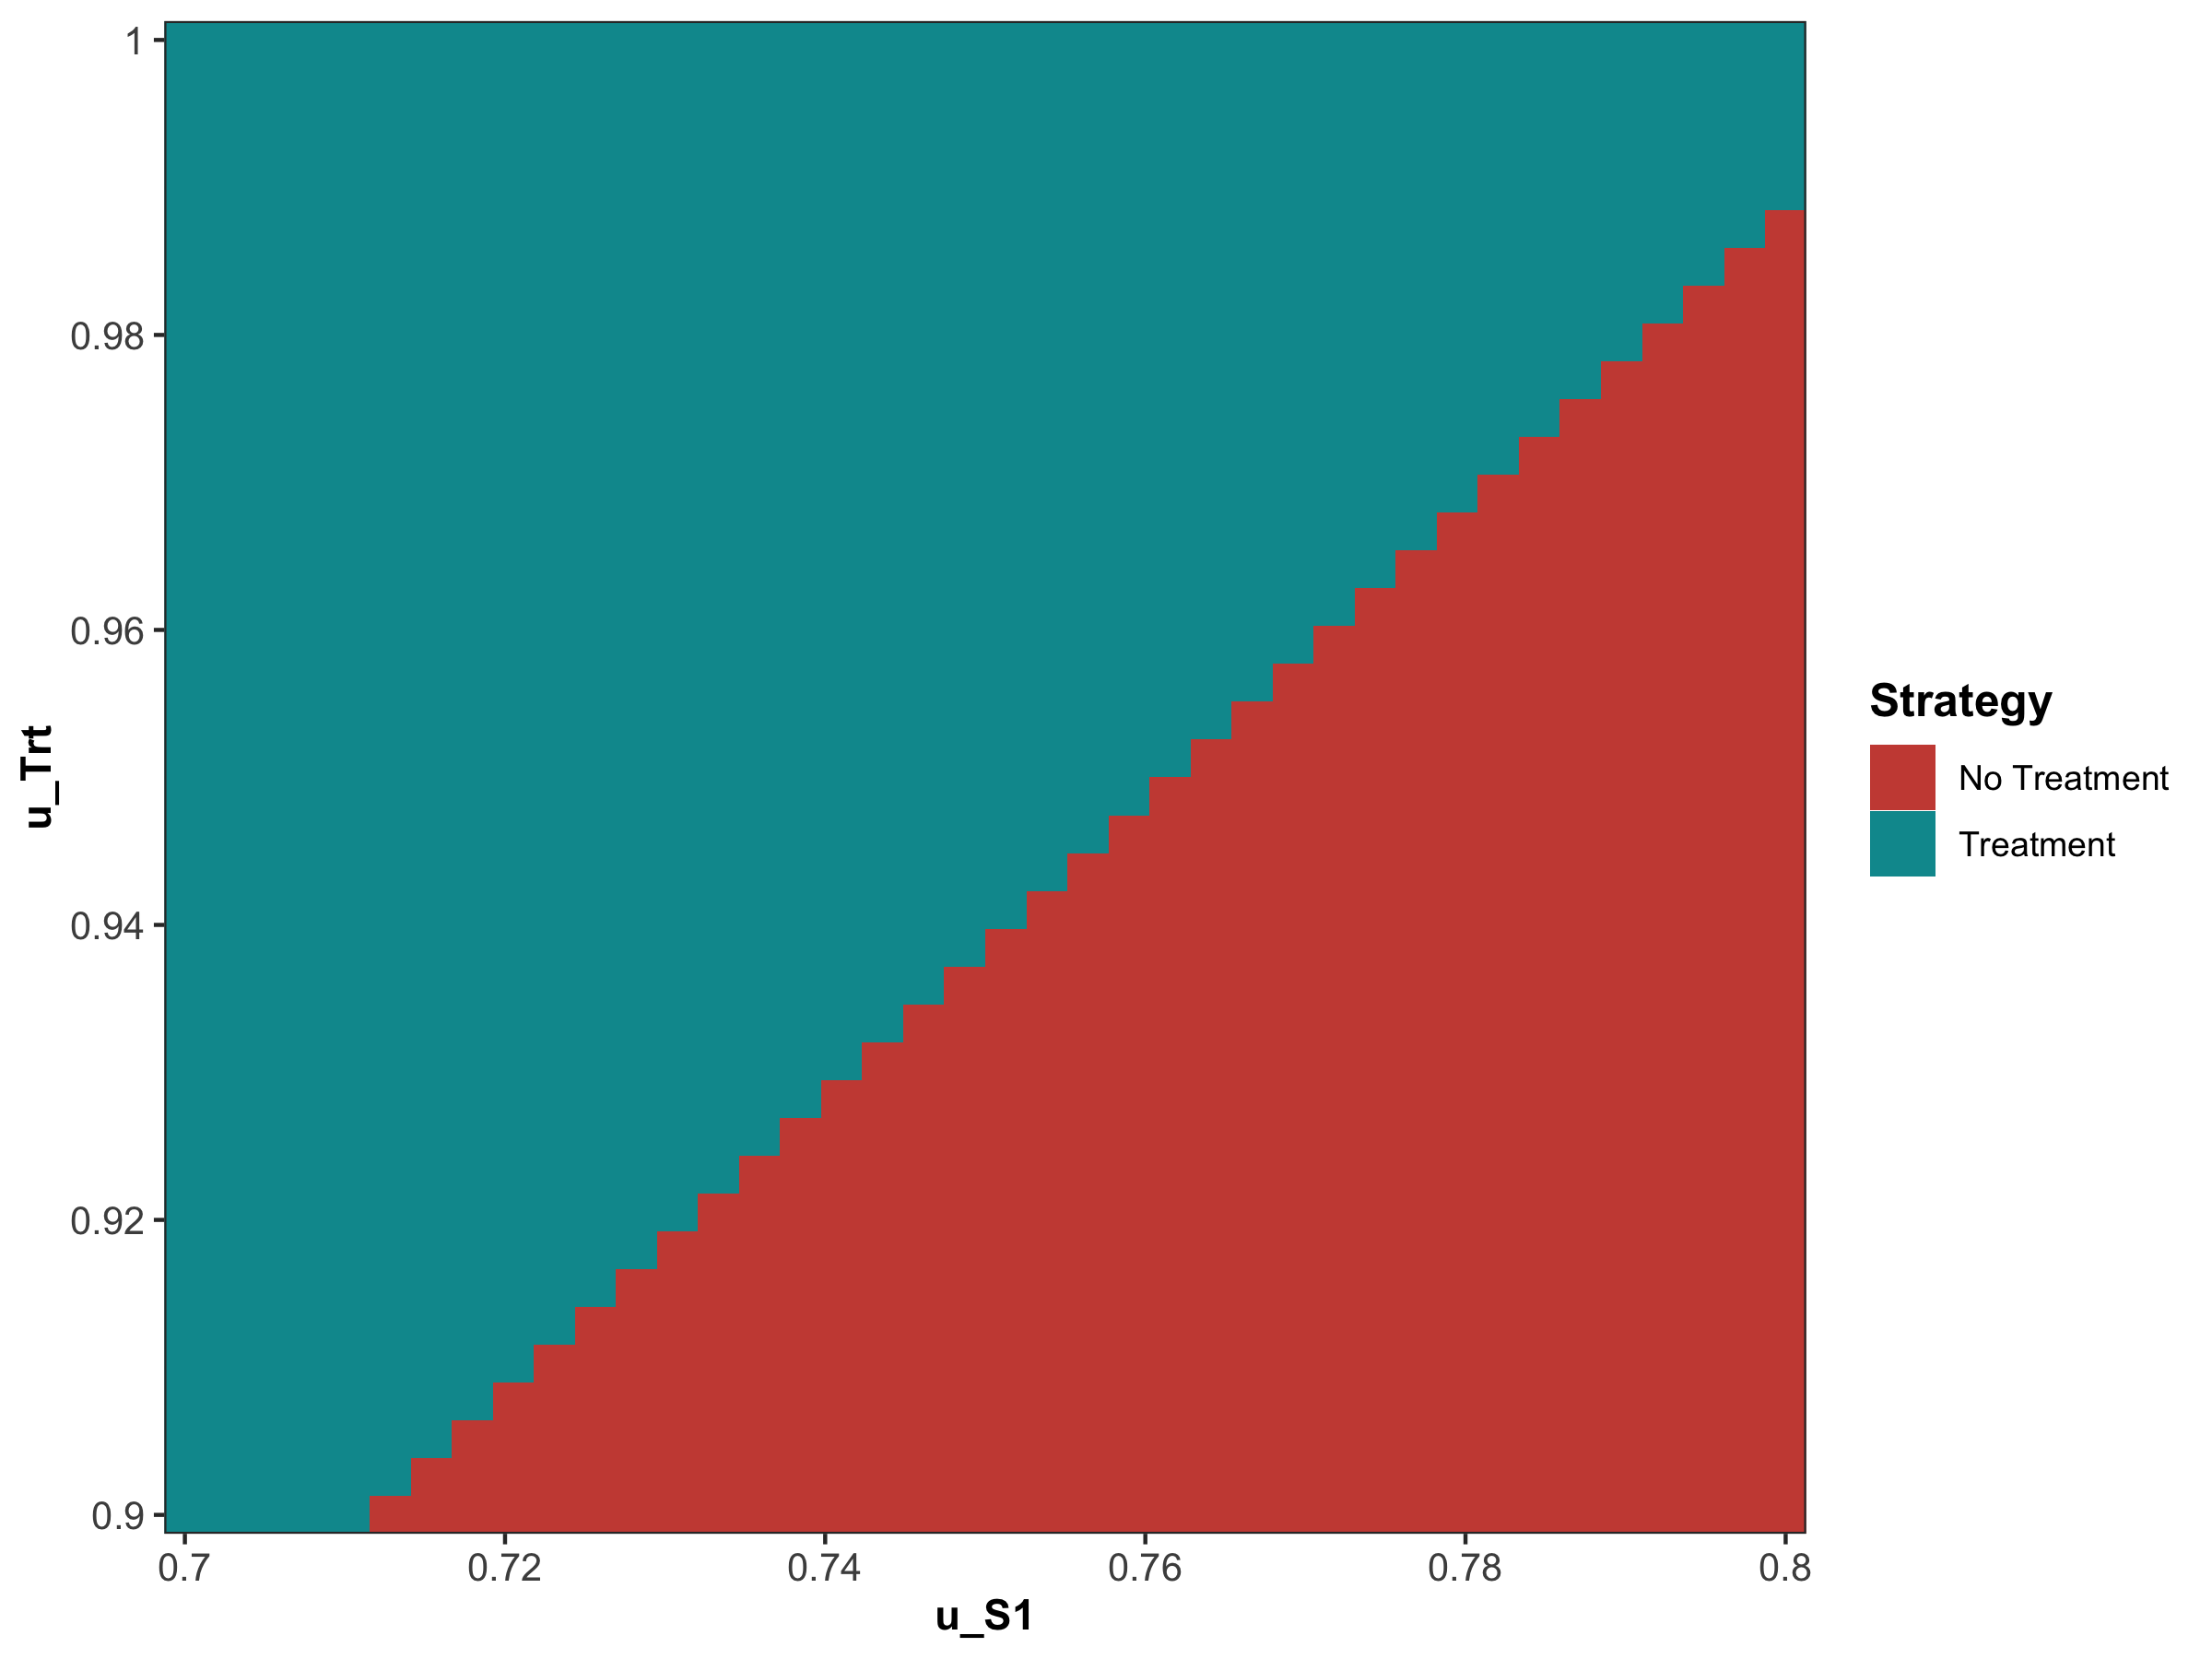
\includegraphics[width=33.33in]{../figs/05a_twsa_uS1_uTrt_nmb} 

}

\caption{Two-way sensitivity results.}\label{fig:05a-twsa-uS1-uTrt-nmb}
\end{figure}

\section{05b Probabilistic analysis}\label{Probabilistic-analysis}

In this subcomponent, we evaluate decision uncertainty by propagating
the uncertainty through the CEA using probabilistic sensitivity analysis
(PSA). Until now we used the parameter values as described in Table
\ref{tab:parameters}. However, we are uncertain about these values. Most
of these input parameters are defined by probability distribution as
described in Table \ref{tab:parameters-PSA}.

\begin{longtable}[]{@{}lcc@{}}
\caption{\label{tab:parameters-PSA} Description of parameters with their R
name and distribution.}\tabularnewline
\toprule
\begin{minipage}[b]{0.43\columnwidth}\raggedright\strut
\textbf{Parameter}\strut
\end{minipage} & \begin{minipage}[b]{0.18\columnwidth}\centering\strut
\textbf{R name}\strut
\end{minipage} & \begin{minipage}[b]{0.20\columnwidth}\centering\strut
\textbf{Distribution}\strut
\end{minipage}\tabularnewline
\midrule
\endfirsthead
\toprule
\begin{minipage}[b]{0.43\columnwidth}\raggedright\strut
\textbf{Parameter}\strut
\end{minipage} & \begin{minipage}[b]{0.18\columnwidth}\centering\strut
\textbf{R name}\strut
\end{minipage} & \begin{minipage}[b]{0.20\columnwidth}\centering\strut
\textbf{Distribution}\strut
\end{minipage}\tabularnewline
\midrule
\endhead
\begin{minipage}[t]{0.43\columnwidth}\raggedright\strut
Annual transition probabilities\strut
\end{minipage} & \begin{minipage}[t]{0.18\columnwidth}\centering\strut
\strut
\end{minipage} & \begin{minipage}[t]{0.20\columnwidth}\centering\strut
\strut
\end{minipage}\tabularnewline
\begin{minipage}[t]{0.43\columnwidth}\raggedright\strut
- Disease onset (H to S1)\strut
\end{minipage} & \begin{minipage}[t]{0.18\columnwidth}\centering\strut
\texttt{p\_HS1}\strut
\end{minipage} & \begin{minipage}[t]{0.20\columnwidth}\centering\strut
\texttt{beta(30,\ 170)}\strut
\end{minipage}\tabularnewline
\begin{minipage}[t]{0.43\columnwidth}\raggedright\strut
- Recovery (S1 to H)\strut
\end{minipage} & \begin{minipage}[t]{0.18\columnwidth}\centering\strut
\texttt{p\_S1H}\strut
\end{minipage} & \begin{minipage}[t]{0.20\columnwidth}\centering\strut
\texttt{beta(60,\ 60)}\strut
\end{minipage}\tabularnewline
\begin{minipage}[t]{0.43\columnwidth}\raggedright\strut
Annual costs\strut
\end{minipage} & \begin{minipage}[t]{0.18\columnwidth}\centering\strut
\strut
\end{minipage} & \begin{minipage}[t]{0.20\columnwidth}\centering\strut
\strut
\end{minipage}\tabularnewline
\begin{minipage}[t]{0.43\columnwidth}\raggedright\strut
- Healthy individuals\strut
\end{minipage} & \begin{minipage}[t]{0.18\columnwidth}\centering\strut
\texttt{c\_H}\strut
\end{minipage} & \begin{minipage}[t]{0.20\columnwidth}\centering\strut
\texttt{gamma(shape\ =\ 100,\ scale\ =\ 20)}\strut
\end{minipage}\tabularnewline
\begin{minipage}[t]{0.43\columnwidth}\raggedright\strut
- Sick individuals in S1\strut
\end{minipage} & \begin{minipage}[t]{0.18\columnwidth}\centering\strut
\texttt{c\_S1}\strut
\end{minipage} & \begin{minipage}[t]{0.20\columnwidth}\centering\strut
\texttt{gamma(shape\ =\ 177.8,\ scale\ =\ 22.5)}\strut
\end{minipage}\tabularnewline
\begin{minipage}[t]{0.43\columnwidth}\raggedright\strut
- Sick individuals in S2\strut
\end{minipage} & \begin{minipage}[t]{0.18\columnwidth}\centering\strut
\texttt{c\_S2}\strut
\end{minipage} & \begin{minipage}[t]{0.20\columnwidth}\centering\strut
\texttt{gamma(shape\ =\ 225,\ scale\ =\ 66.7)}\strut
\end{minipage}\tabularnewline
\begin{minipage}[t]{0.43\columnwidth}\raggedright\strut
- Additional costs of sick individuals treated in S1 or S2\strut
\end{minipage} & \begin{minipage}[t]{0.18\columnwidth}\centering\strut
\texttt{c.Trt}\strut
\end{minipage} & \begin{minipage}[t]{0.20\columnwidth}\centering\strut
\texttt{gamma(shape\ =\ 73.5,\ scale\ =\ 163.3)}\strut
\end{minipage}\tabularnewline
\begin{minipage}[t]{0.43\columnwidth}\raggedright\strut
Utility weights\strut
\end{minipage} & \begin{minipage}[t]{0.18\columnwidth}\centering\strut
\strut
\end{minipage} & \begin{minipage}[t]{0.20\columnwidth}\centering\strut
\strut
\end{minipage}\tabularnewline
\begin{minipage}[t]{0.43\columnwidth}\raggedright\strut
- Healthy individuals\strut
\end{minipage} & \begin{minipage}[t]{0.18\columnwidth}\centering\strut
\texttt{u\_H}\strut
\end{minipage} & \begin{minipage}[t]{0.20\columnwidth}\centering\strut
\texttt{truncnorm(mean\ =\ 1,\ sd\ =\ 0.01,\ b\ =\ 1)}\strut
\end{minipage}\tabularnewline
\begin{minipage}[t]{0.43\columnwidth}\raggedright\strut
- Sick individuals in S1\strut
\end{minipage} & \begin{minipage}[t]{0.18\columnwidth}\centering\strut
\texttt{u\_S1}\strut
\end{minipage} & \begin{minipage}[t]{0.20\columnwidth}\centering\strut
\texttt{truncnorm(mean\ =\ 0.75,\ sd\ =\ 0.02,\ b\ =\ 1)}\strut
\end{minipage}\tabularnewline
\begin{minipage}[t]{0.43\columnwidth}\raggedright\strut
- Sick individuals in S2\strut
\end{minipage} & \begin{minipage}[t]{0.18\columnwidth}\centering\strut
\texttt{u\_S2}\strut
\end{minipage} & \begin{minipage}[t]{0.20\columnwidth}\centering\strut
\texttt{truncnorm(mean\ =\ 0.50,\ sd\ =\ 0.03,\ b\ =\ 1)}\strut
\end{minipage}\tabularnewline
\begin{minipage}[t]{0.43\columnwidth}\raggedright\strut
Intervention effect\strut
\end{minipage} & \begin{minipage}[t]{0.18\columnwidth}\centering\strut
\strut
\end{minipage} & \begin{minipage}[t]{0.20\columnwidth}\centering\strut
\strut
\end{minipage}\tabularnewline
\begin{minipage}[t]{0.43\columnwidth}\raggedright\strut
- Utility for treated individuals in S1\strut
\end{minipage} & \begin{minipage}[t]{0.18\columnwidth}\centering\strut
\texttt{u\_Trt}\strut
\end{minipage} & \begin{minipage}[t]{0.20\columnwidth}\centering\strut
\texttt{truncnorm(mean\ =\ 0.95,\ sd\ =\ 0.02,\ b\ =\ 1)}\strut
\end{minipage}\tabularnewline
\bottomrule
\end{longtable}

In a PSA we sample the input parameter values from these distributions
and we then run the model at each sample. In the file
\emph{05b\_uncertainty\_analysis\_functions.R} we created a single
function, called \texttt{generate\_psa\_params}. This function generates
a PSA dataset for all the CEA input parameters. We specify the number of
PSA samples via the \texttt{n\_sim} argument. The function also accepts
specifying a seed to allow reproducibility of the results.

\begin{Shaded}
\begin{Highlighting}[]
\KeywordTok{print.function}\NormalTok{(generate_psa_params) }\CommentTok{# print the function }
\end{Highlighting}
\end{Shaded}

\begin{verbatim}
## function(n_sim = 1000, seed = 20190220){ # User defined
##   ## Load calibrated parameters
##   data("m_calib_post")
##   n_sim <- nrow(m_calib_post)
##   set_seed <- seed
##   df_psa_params <- data.frame(
##     ### Calibrated parameters
##     m_calib_post,
##     
##     ### Transition probabilities (per cycle)
##     p_HS1   = rbeta(n_sim, 30, 170),        # probability to become sick when healthy
##     p_S1H   = rbeta(n_sim, 60, 60) ,        # probability to become healthy when sick
##     
##     ### State rewards
##     ## Costs
##     c_H   = rgamma(n_sim, shape = 100, scale = 20)    , # cost of remaining one cycle in state H
##     c_S1  = rgamma(n_sim, shape = 177.8, scale = 22.5), # cost of remaining one cycle in state S1
##     c_S2  = rgamma(n_sim, shape = 225, scale = 66.7)  , # cost of remaining one cycle in state S2
##     c_Trt = rgamma(n_sim, shape = 73.5, scale = 163.3), # cost of treatment (per cycle)
##     c_D   = 0                                         , # cost of being in the death state
##     ## Utilities
##     u_H   = truncnorm::rtruncnorm(n_sim, mean =    1, sd = 0.01, b = 1), # utility when healthy
##     u_S1  = truncnorm::rtruncnorm(n_sim, mean = 0.75, sd = 0.02, b = 1), # utility when sick
##     u_S2  = truncnorm::rtruncnorm(n_sim, mean = 0.50, sd = 0.03, b = 1), # utility when sicker
##     u_D   = 0                                               , # utility when dead
##     u_Trt = truncnorm::rtruncnorm(n_sim, mean = 0.95, sd = 0.02, b = 1)  # utility when being treated
##   )
##   return(df_psa_params)
## }
## <bytecode: 0x1177ccb20>
## <environment: namespace:darthpack>
\end{verbatim}

The function returns the \texttt{df\_psa\_input} dataframe with a PSA
dataset of the input parameters. With this dataframe we can run the PSA
to produce distributions of costs, effectiveness and NMB. The PSA is
performed by the \emph{05b\_probabilistic\_analysis.R} script. As shown
in the code below, the \texttt{df\_psa\_input} dataframe is used by the
\texttt{update\_param\_list} function to generate the corresponding list
of parameters for the PSA. For each simulation, we perfrom three steps.
First, the list of parameters is updated by the
\texttt{update\_param\_list} function. Second, the model is executed by
the \texttt{calculate\_ce\_out} function using the updated parameter
list and third, the dataframes \texttt{df\_c} and \texttt{df\_e} store
the estimated cost and effects, respectively. The final part of this
loop is to satisfy the modeler when waiting on the results, by
displaying the simulation progress.

\begin{Shaded}
\begin{Highlighting}[]
\ControlFlowTok{for}\NormalTok{(i }\ControlFlowTok{in} \DecValTok{1}\OperatorTok{:}\NormalTok{n_sim)\{ }
\NormalTok{  l_psa_input <-}\StringTok{ }\KeywordTok{update_param_list}\NormalTok{(l_params_all, df_psa_input[i, ])}
\NormalTok{  df_out_temp <-}\StringTok{ }\KeywordTok{calculate_ce_out}\NormalTok{(l_psa_input)}
\NormalTok{  df_c[i, ] <-}\StringTok{ }\NormalTok{df_out_temp}\OperatorTok{$}\NormalTok{Cost}
\NormalTok{  df_e[i, ] <-}\StringTok{ }\NormalTok{df_out_temp}\OperatorTok{$}\NormalTok{Effect}
  \CommentTok{# Display simulation progress}
  \ControlFlowTok{if}\NormalTok{(i}\OperatorTok{/}\NormalTok{(n_sim}\OperatorTok{/}\DecValTok{10}\NormalTok{) }\OperatorTok{==}\StringTok{ }\KeywordTok{round}\NormalTok{(i}\OperatorTok{/}\NormalTok{(n_sim}\OperatorTok{/}\DecValTok{10}\NormalTok{), }\DecValTok{0}\NormalTok{)) \{}
    \KeywordTok{cat}\NormalTok{(}\StringTok{'}\CharTok{\textbackslash{}r}\StringTok{'}\NormalTok{, }\KeywordTok{paste}\NormalTok{(i}\OperatorTok{/}\NormalTok{n_sim }\OperatorTok{*}\StringTok{ }\DecValTok{100}\NormalTok{, }\StringTok{"% done"}\NormalTok{, }\DataTypeTok{sep =} \StringTok{" "}\NormalTok{))}
\NormalTok{  \}}
\NormalTok{\}}
\end{Highlighting}
\end{Shaded}

We can plot the results using the \texttt{plot} function from
\texttt{dampack}. Figure \ref{fig:05b-CEAplane} shows the CE scatter
plot with the joint distribution of costs and effects for each strategy
and their corresponding 95\% confidence ellipse.

\begin{figure}

{\centering 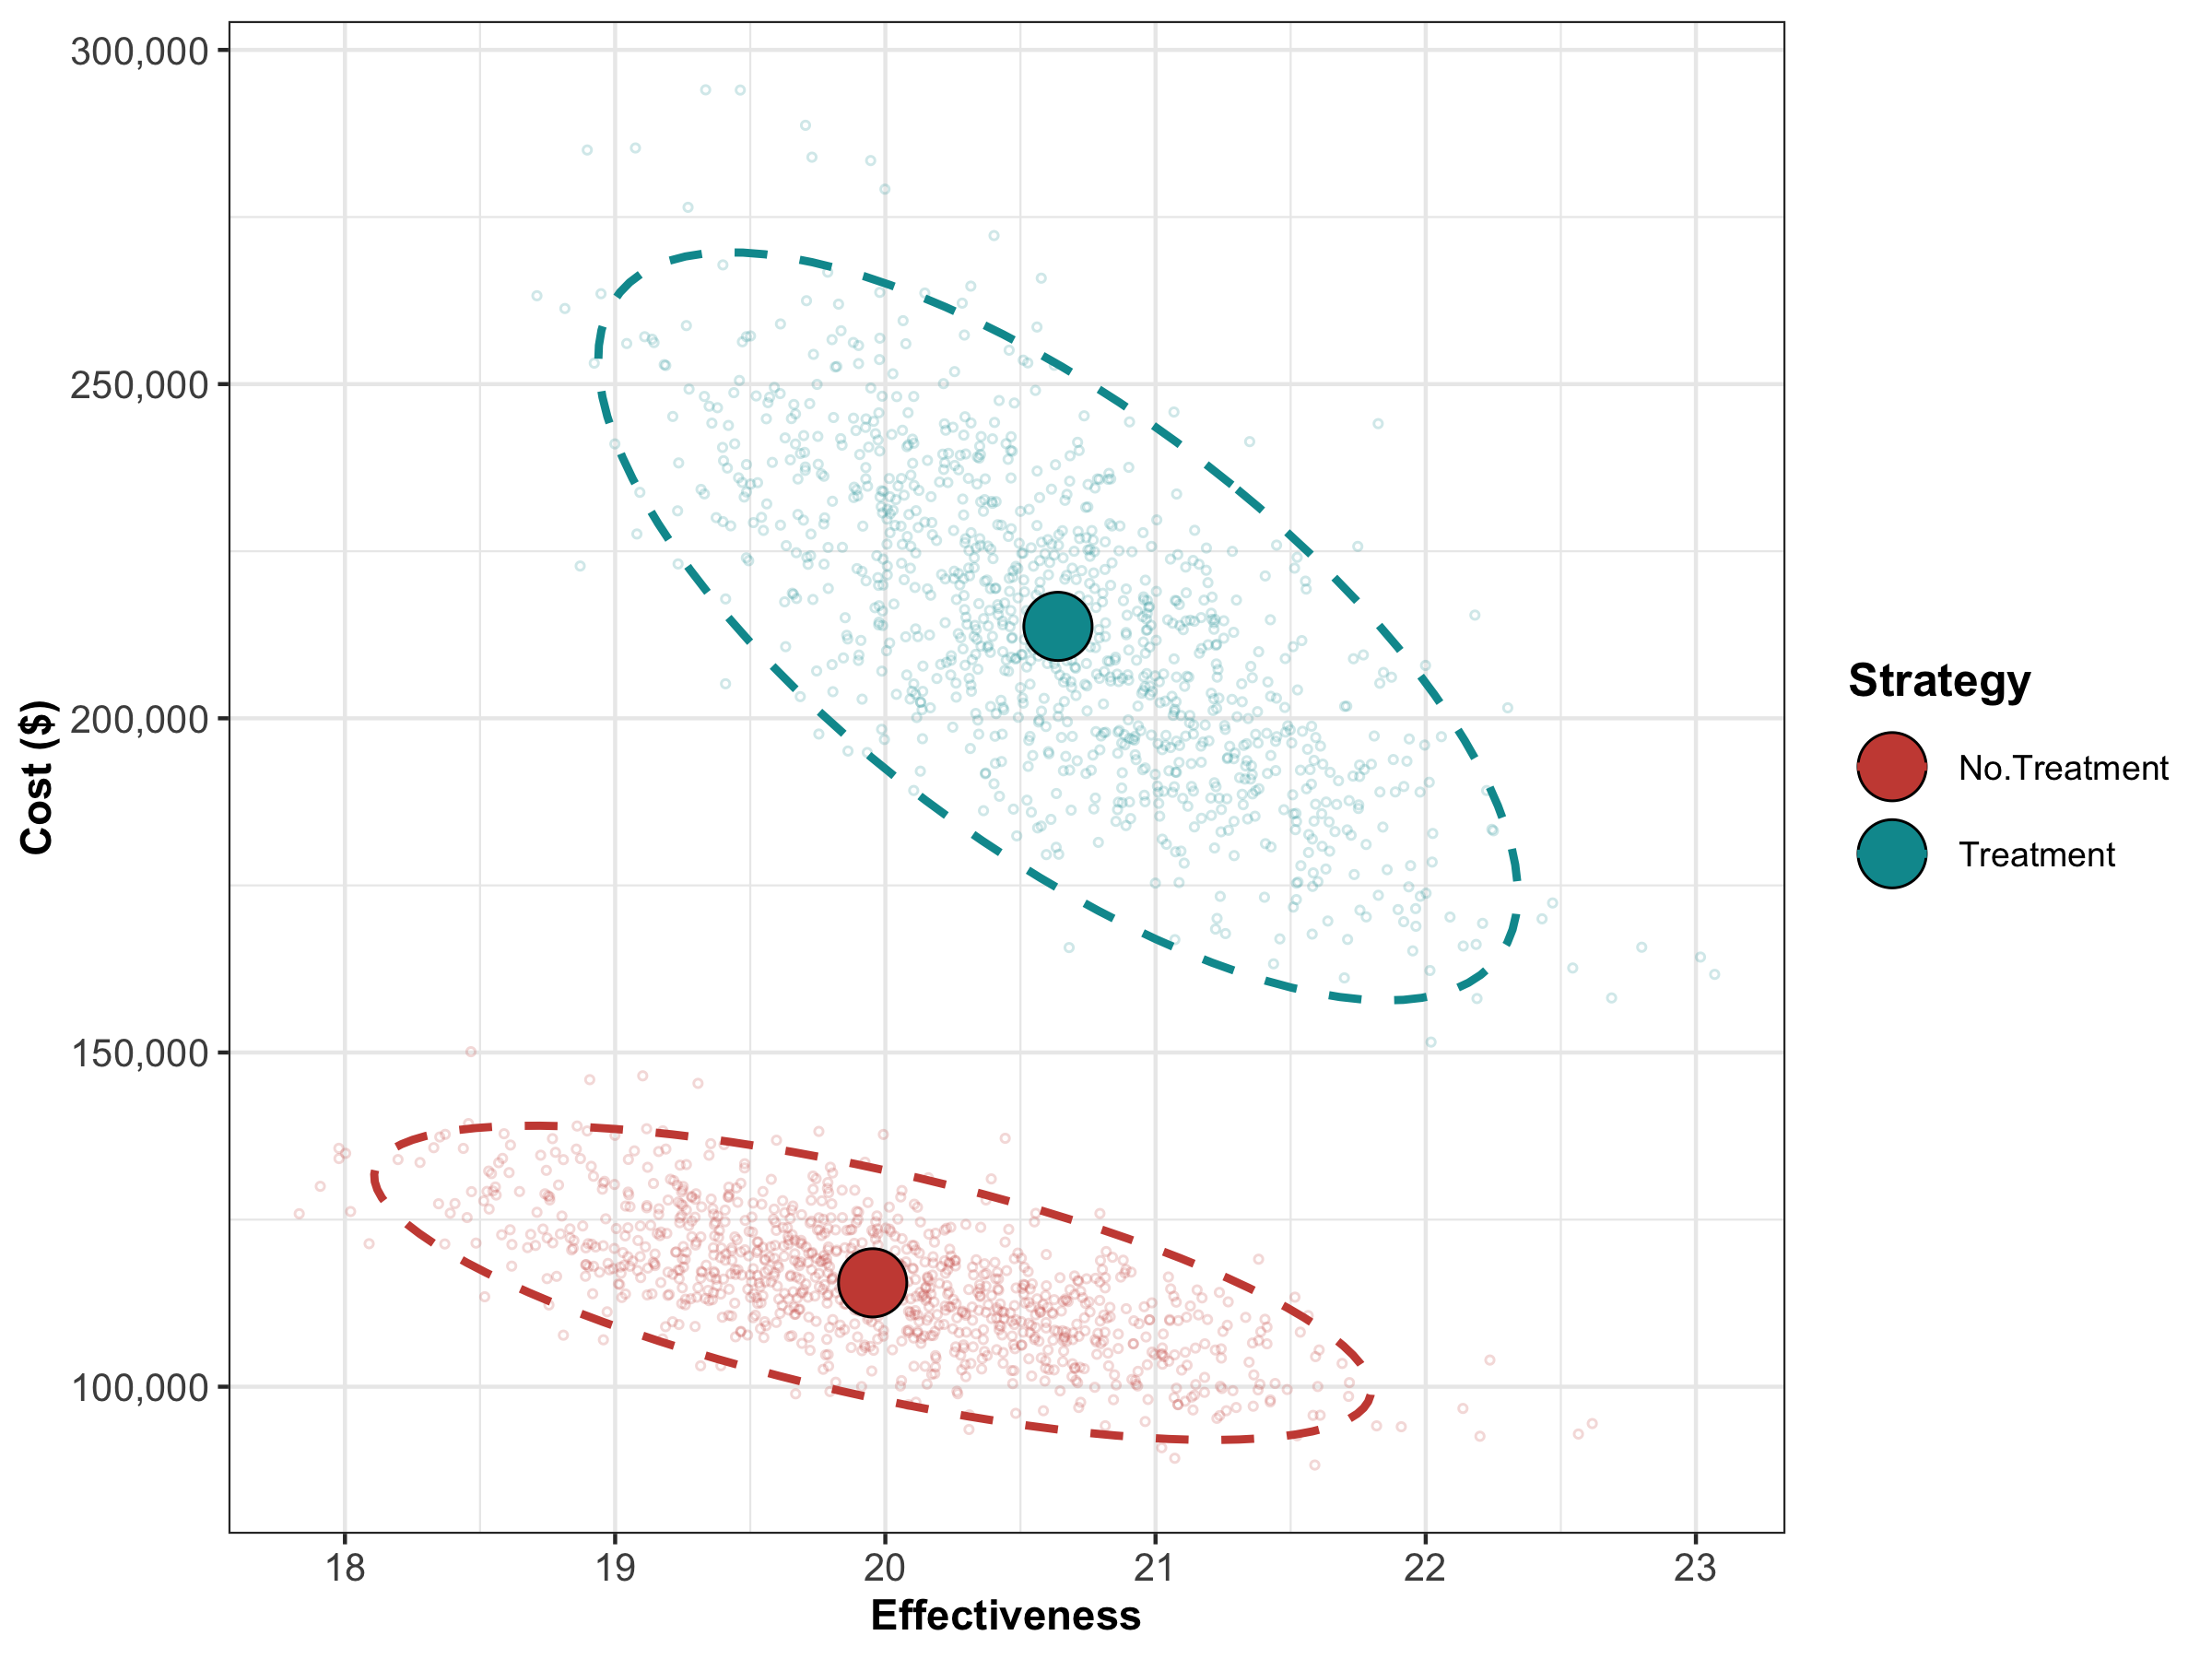
\includegraphics[width=33.33in]{../figs/05b_cea_plane_scatter} 

}

\caption{The cost-effectiveness plane graph showing the results of the probabilistic sensitivity analysis for the Sick-Sicker case-study.}\label{fig:05b-CEAplane}
\end{figure}

\begin{table}[t]

\caption{\label{tab:df-cea-prob}Probabilistic cost-effectiveness analysis results of the Sick-Sicker model comparing no treatment with treatment}
\centering
\begin{tabular}{l|r|r|r|r|r}
\hline
Strategy & Cost & Effect & Inc\_Cost & Inc\_Effect & ICER\\
\hline
No.Treatment & 115538.9 & 19.95305 & NA & NA & NA\\
\hline
Treatment & 213755.8 & 20.63891 & 98216.84 & 0.6858646 & 143201.5\\
\hline
\end{tabular}
\end{table}

Next, we perform a CEA using the previously used
\texttt{calculate\_icers} functions from \texttt{dampack}. Table
\ref{tab:df-cea-prob} shows the results of the probabilistic CEA. In
addition, we plot a cost-effectiveness plane with the frontier, the
cost-effectiveness acceptability curves (CEACs) and frontier (CEAF),
expected Loss curves (ELCs) (Figure @ref(fig:05b\_cea\_frontier\_psa) -
\ref{fig:05b-elc}) \citep{Alarid-Escudero2019}. Followed by creating
linear regression metamodeling sensitivity analysis graphs (Figure
\ref{fig:05b-owsa-lrm-nmb} -
@ref(fig:05b-twsa-lrm-uS1-uTrt\_nmb))\citep{Jalal2013}. All generated
figures are shown below and stored to the \emph{figs} folder .

\begin{figure}

{\centering 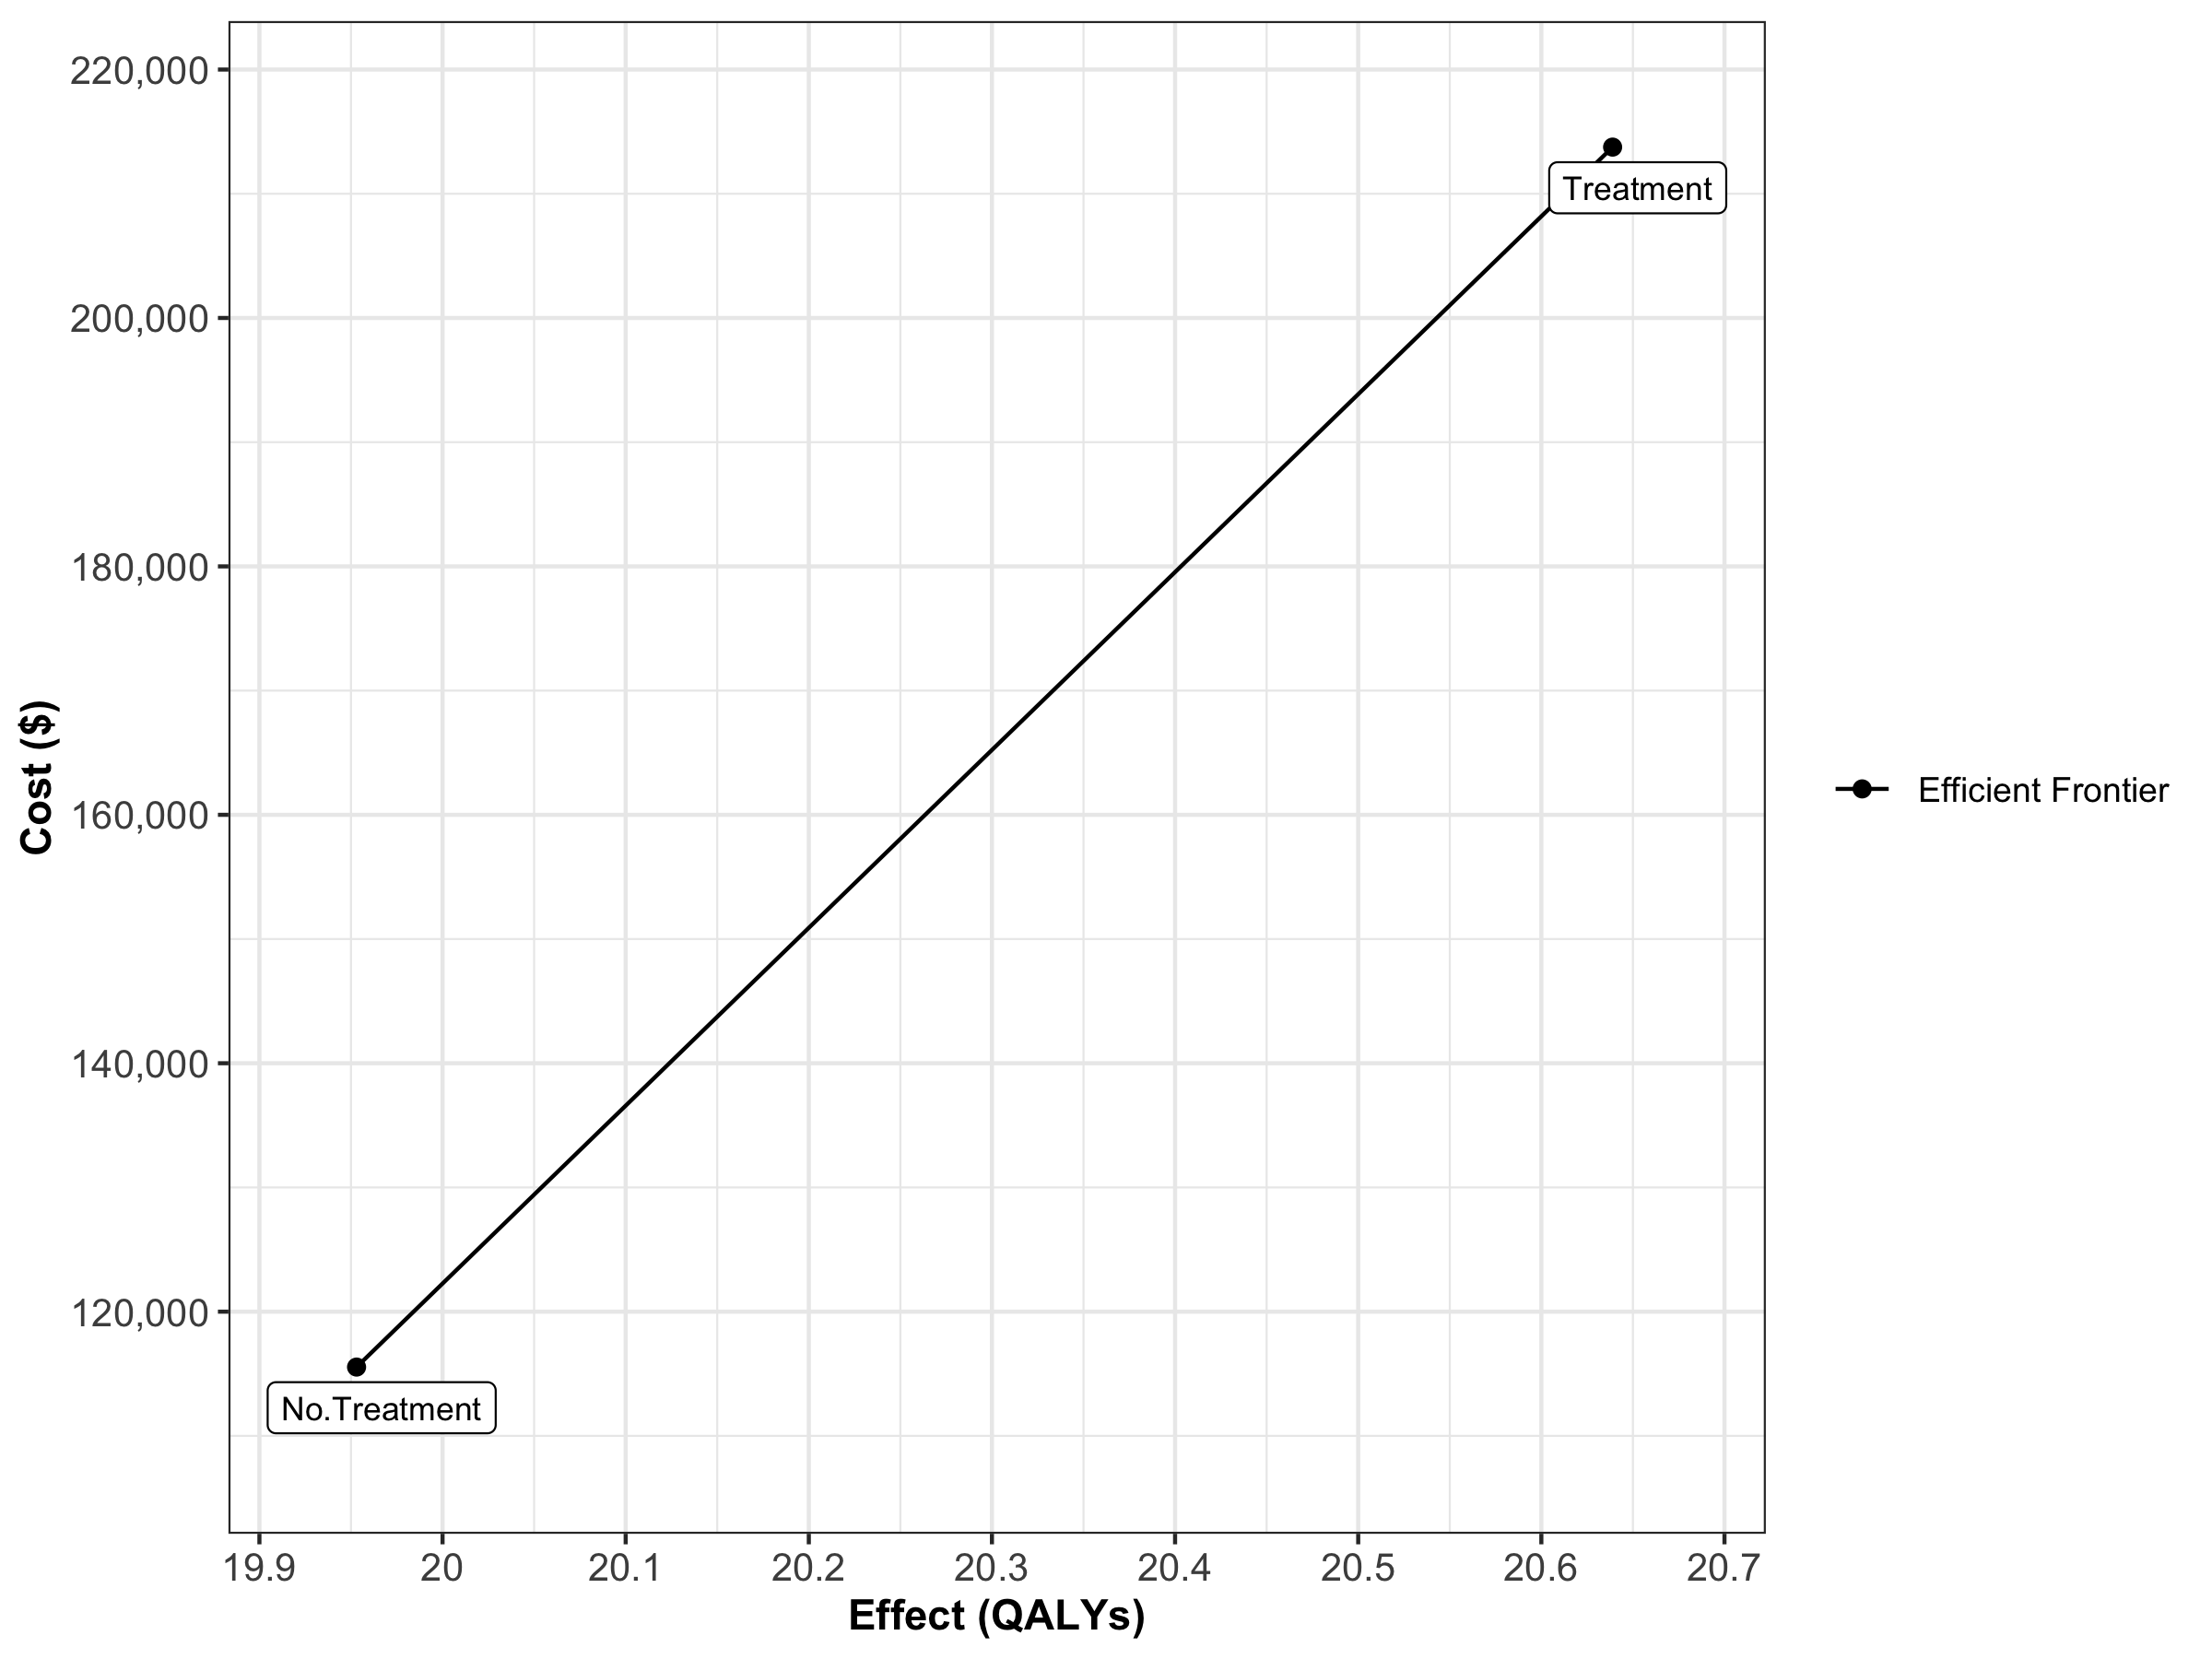
\includegraphics[width=33.33in]{../figs/05b_cea_frontier_psa} 

}

\caption{Cost-effectiveness frontier}\label{fig:05b-cea-frontier-psa}
\end{figure}

\begin{figure}

{\centering 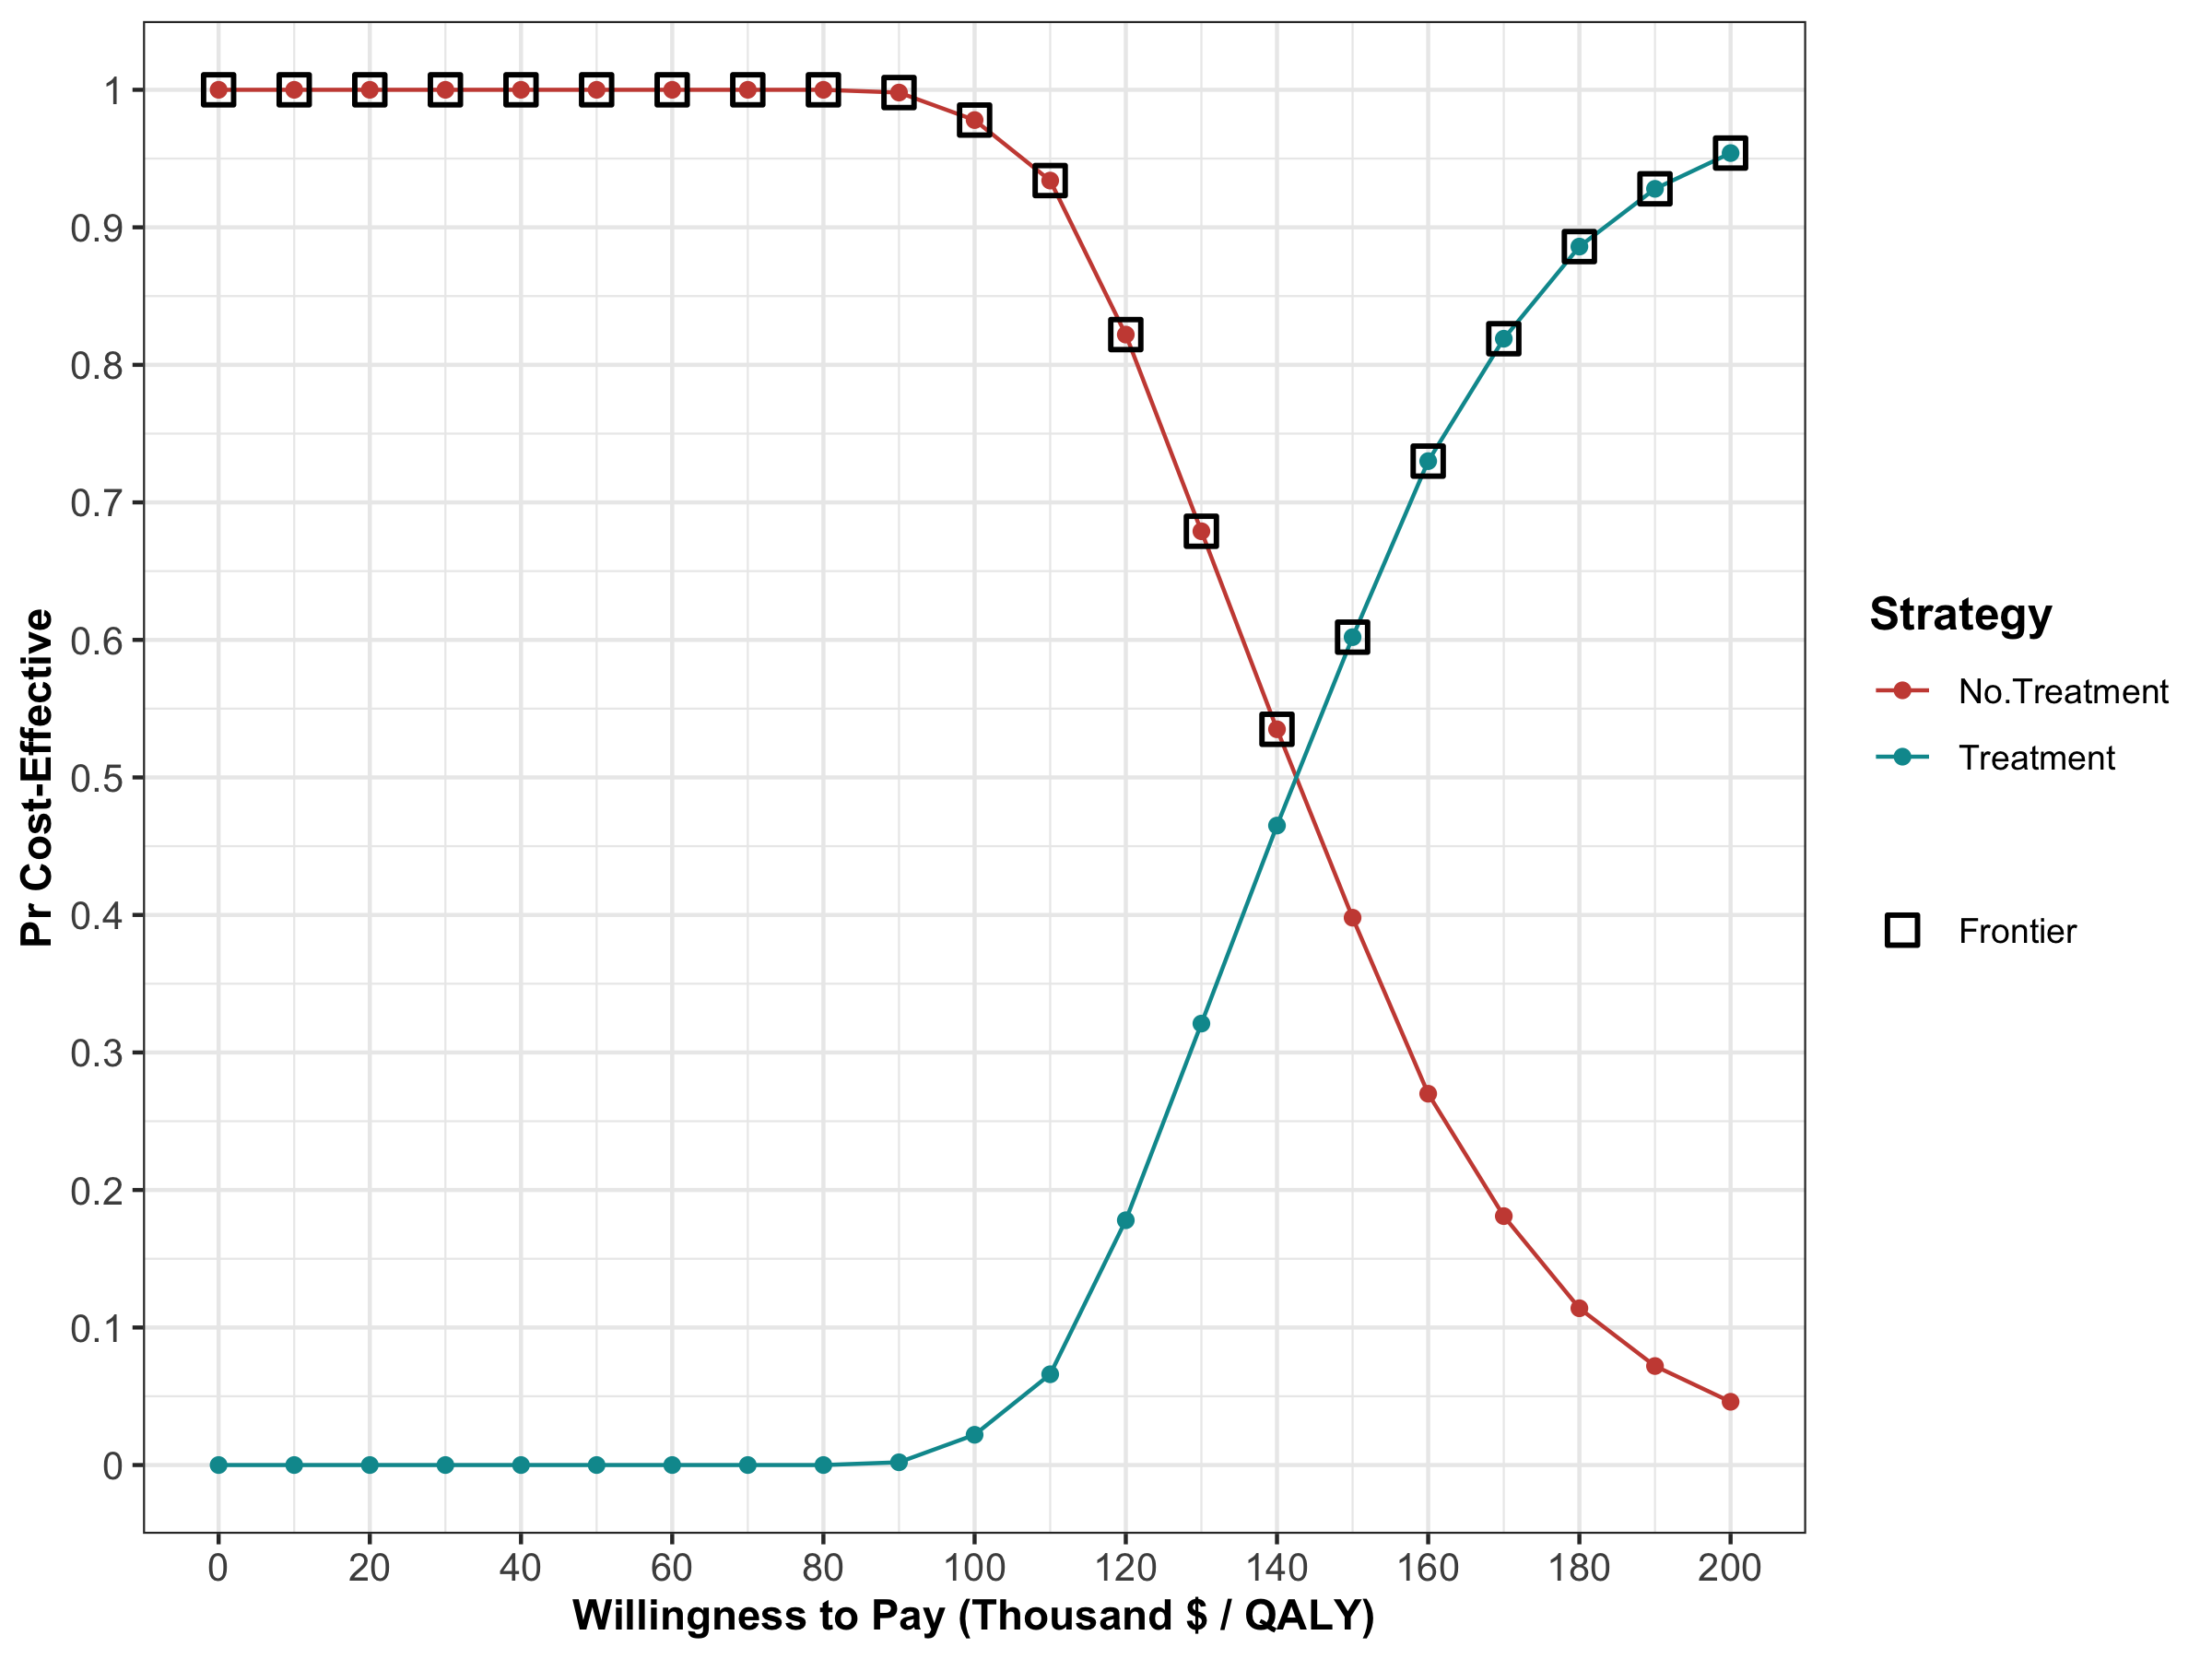
\includegraphics[width=33.33in]{../figs/05b_ceac_ceaf} 

}

\caption{Cost-effectiveness acceptability curves (CEACs) and frontier (CEAF).}\label{fig:05b-ceac-ceaf}
\end{figure}

\begin{figure}

{\centering 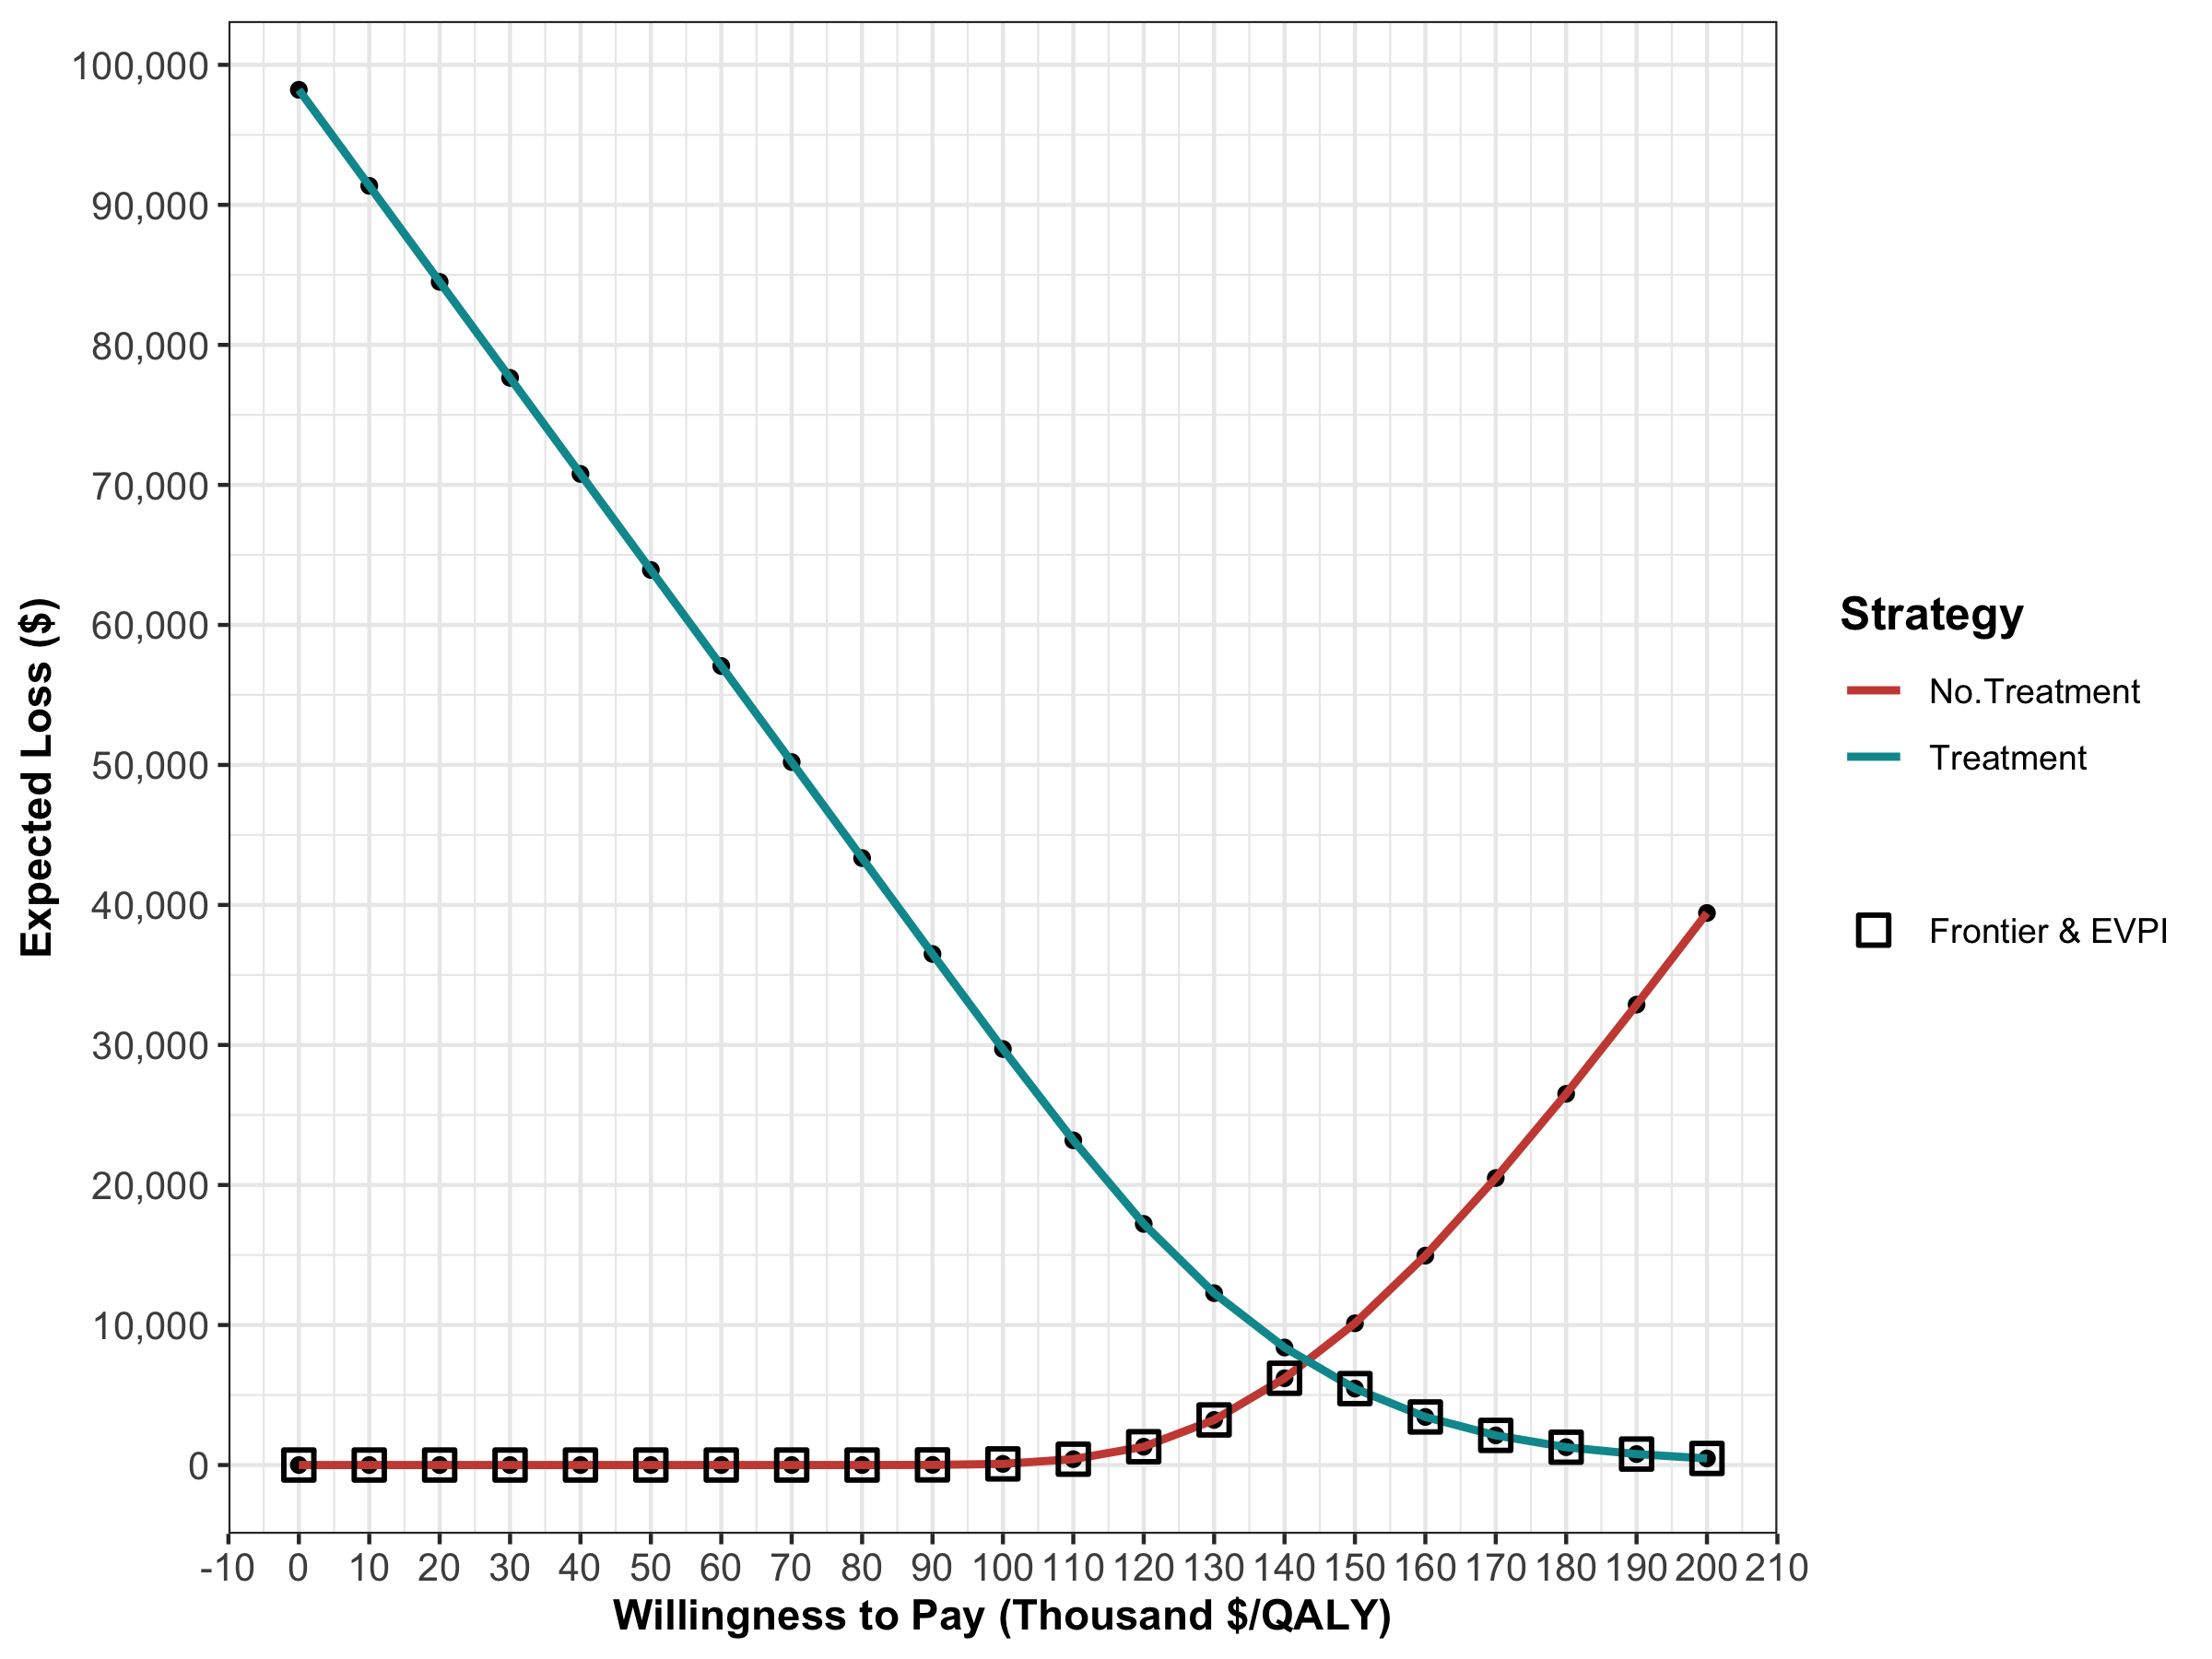
\includegraphics[width=33.33in]{../figs/05b_elc} 

}

\caption{Expected Loss Curves.}\label{fig:05b-elc}
\end{figure}

\begin{figure}

{\centering 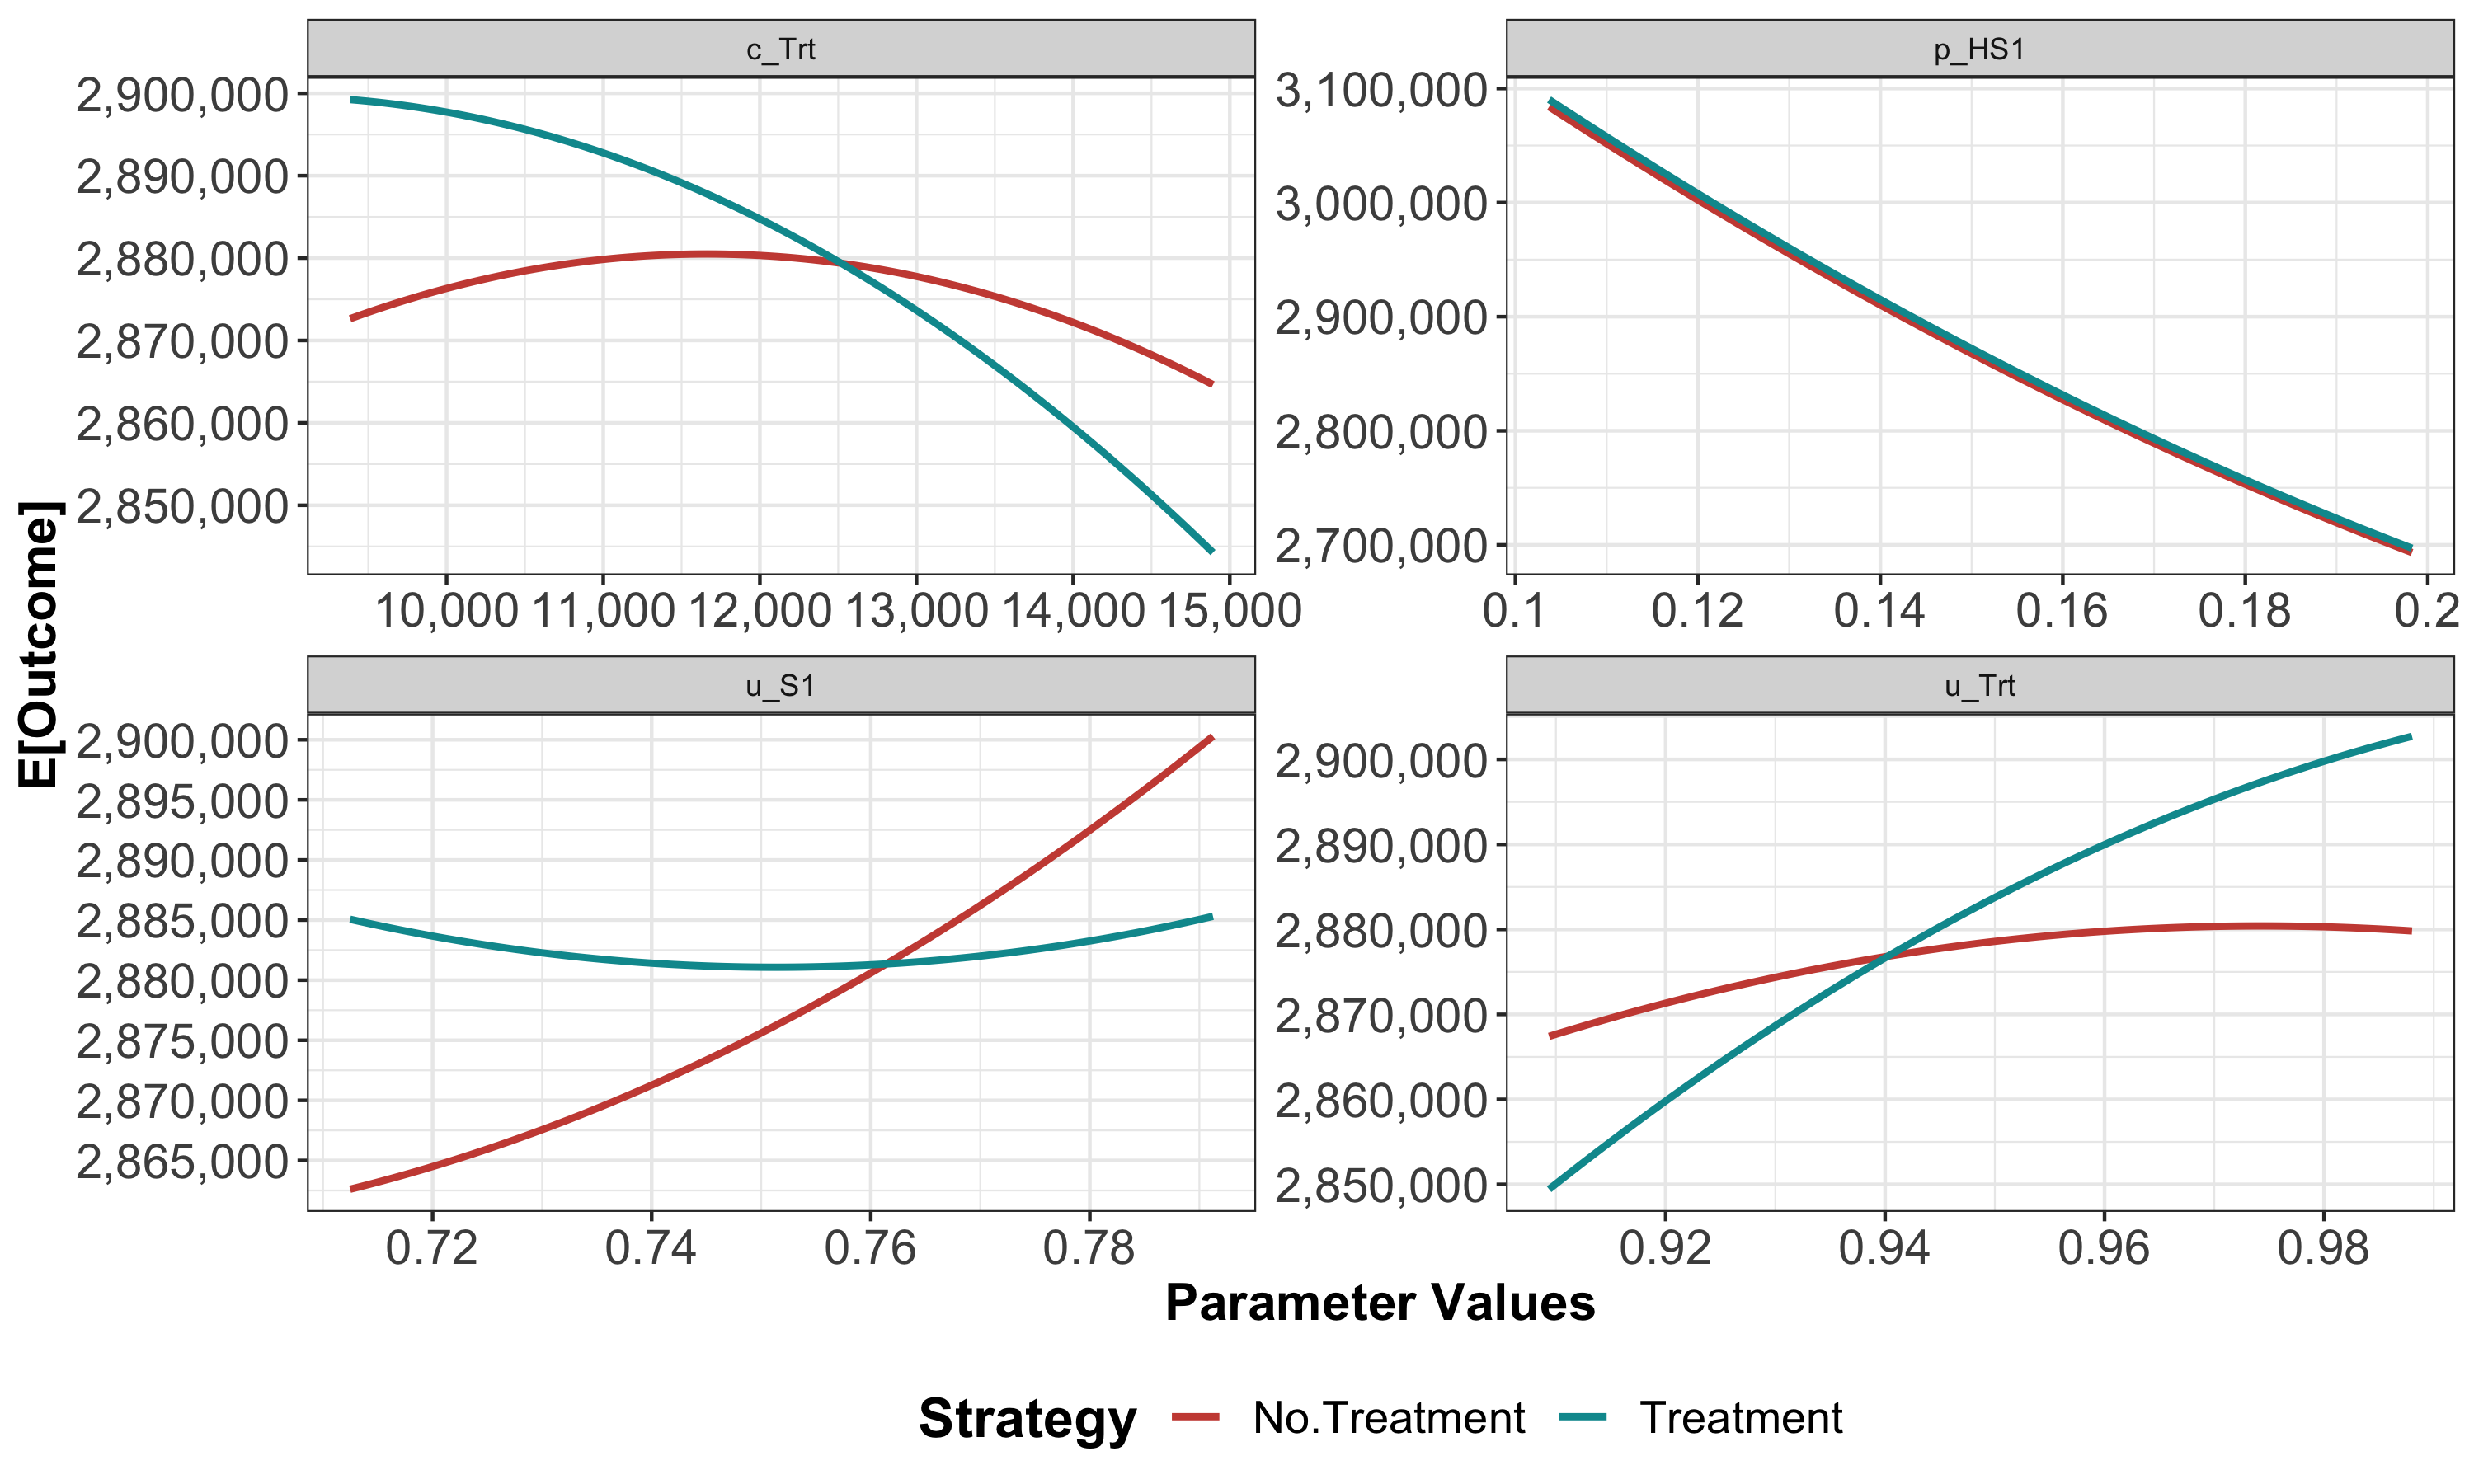
\includegraphics[width=41.67in]{../figs/05b_owsa_lrm_nmb} 

}

\caption{One-way sensitivity analysis (OWSA).}\label{fig:05b-owsa-lrm-nmb}
\end{figure}

\begin{figure}

{\centering 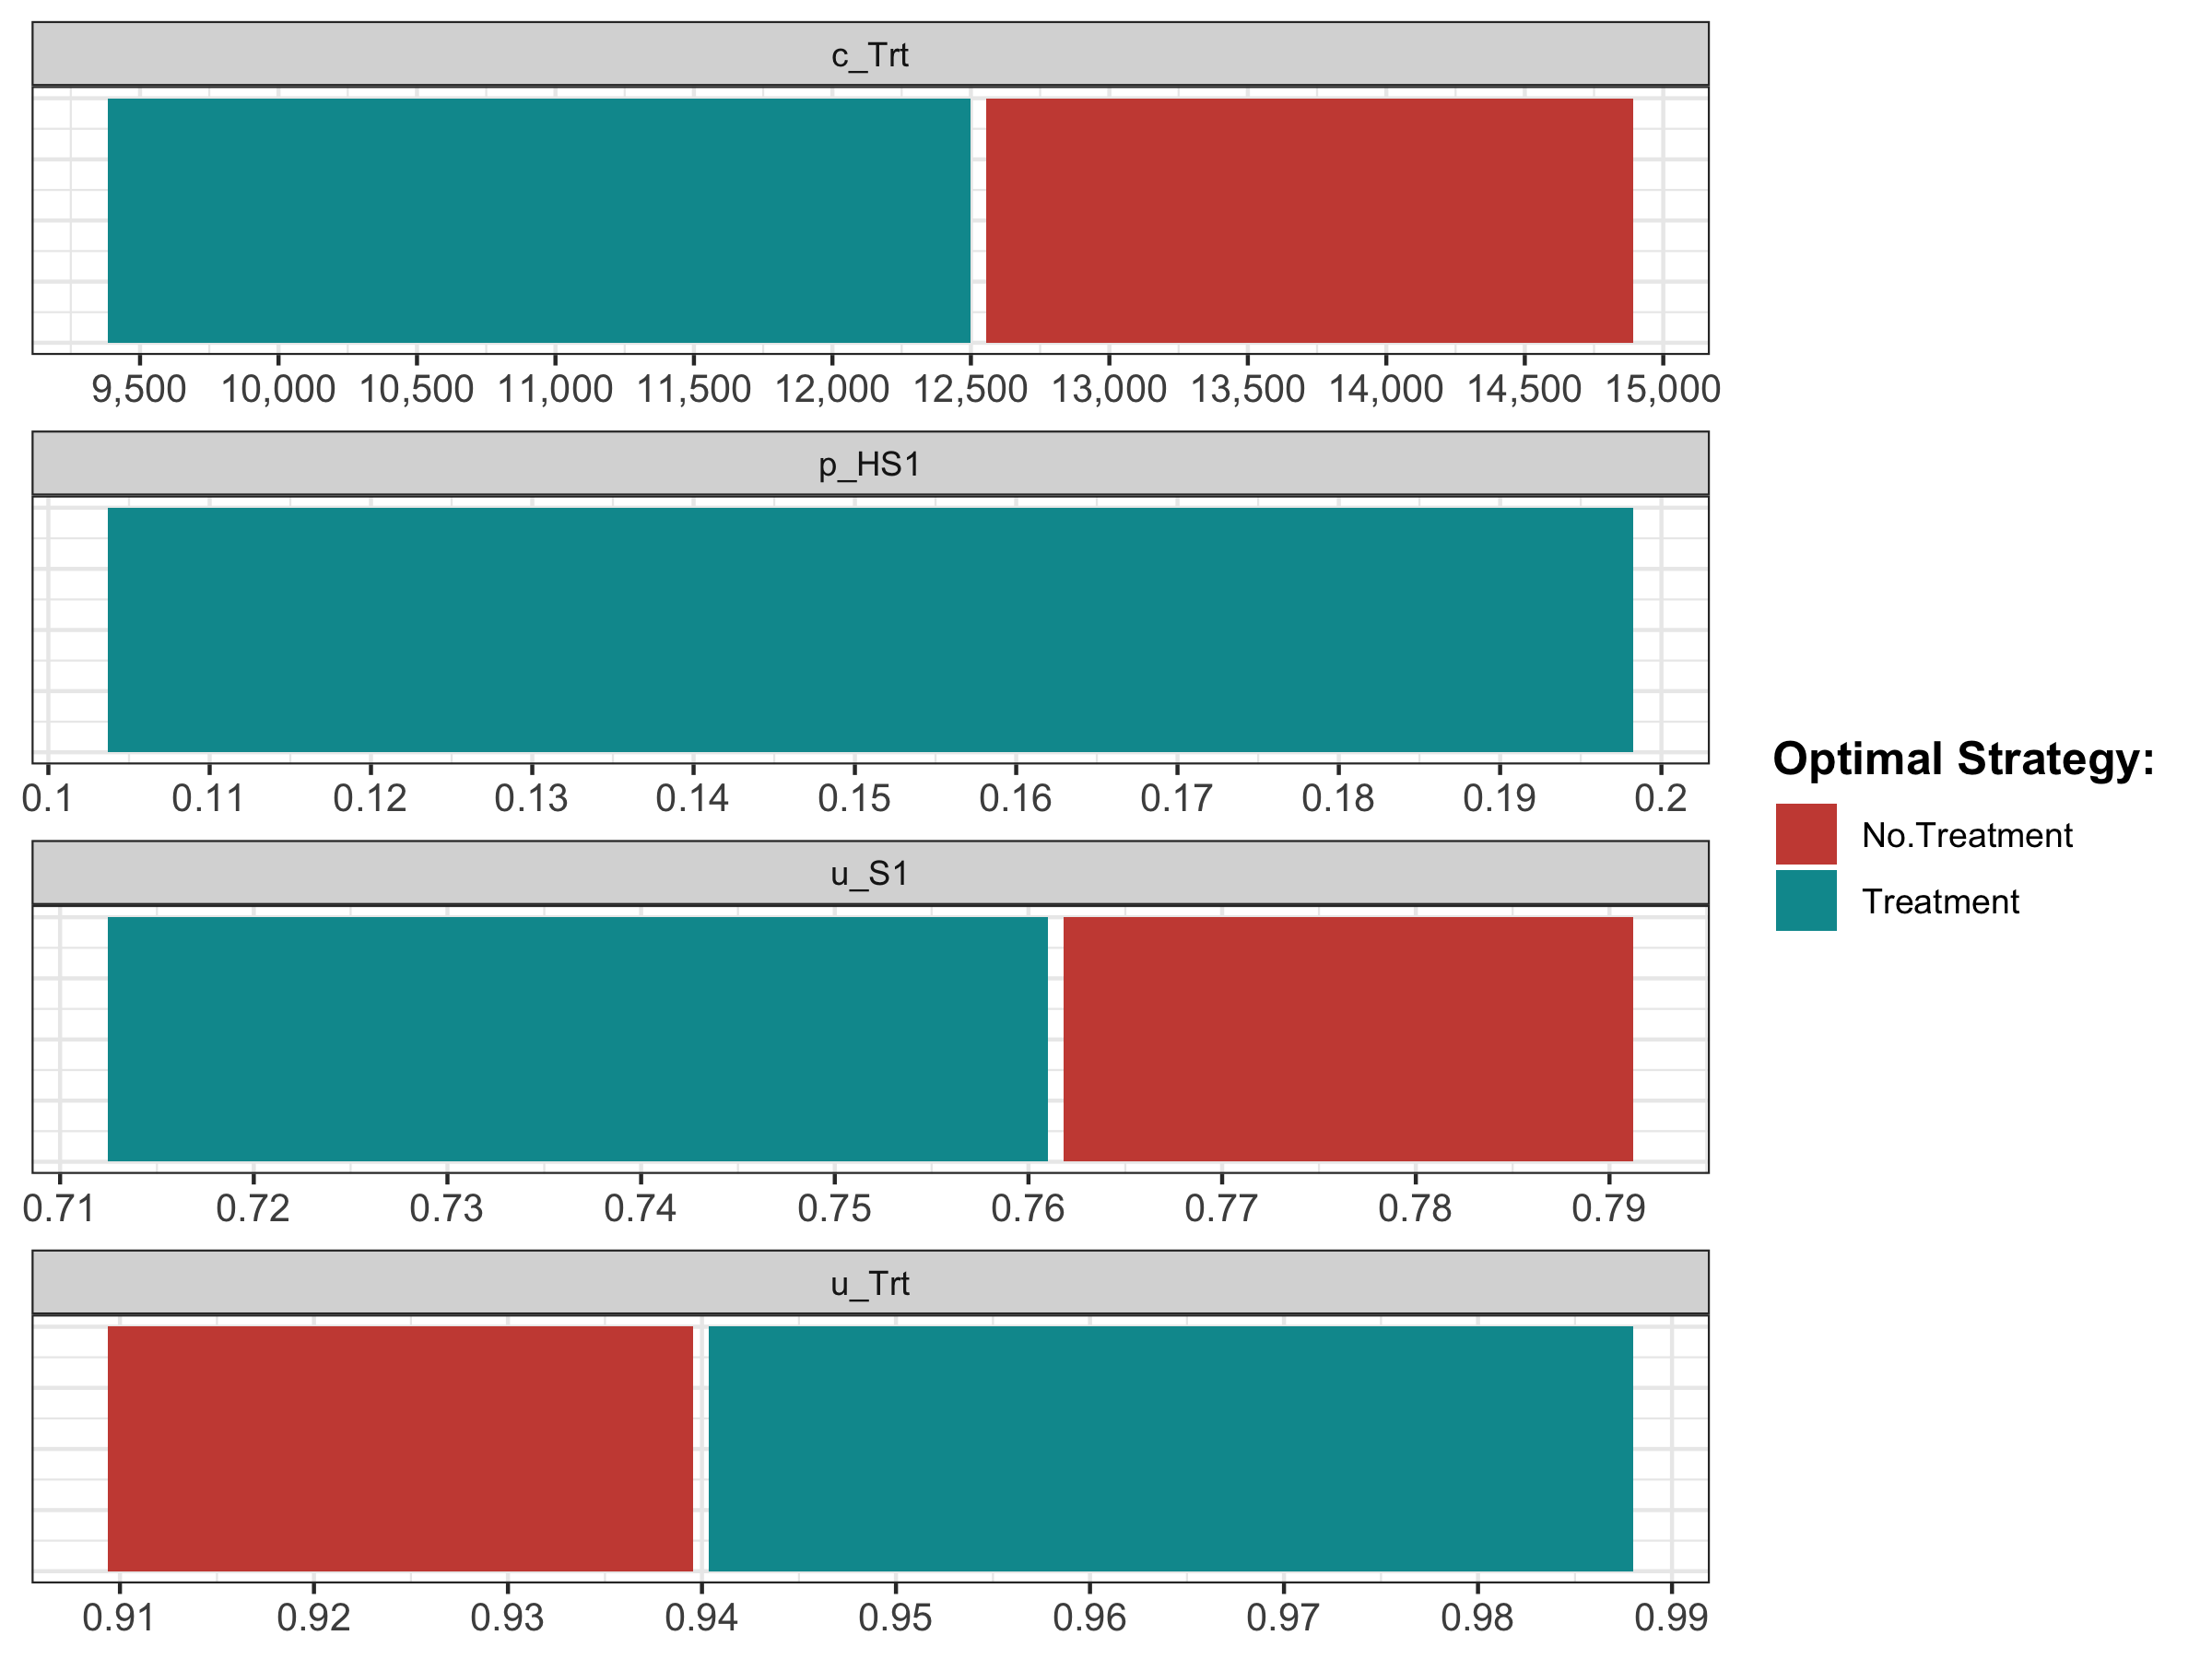
\includegraphics[width=33.33in]{../figs/05b_optimal_owsa_lrm_nmb} 

}

\caption{Optimal strategy with OWSA}\label{fig:05b-optimal-owsa-lrm-nmb}
\end{figure}

\begin{figure}

{\centering 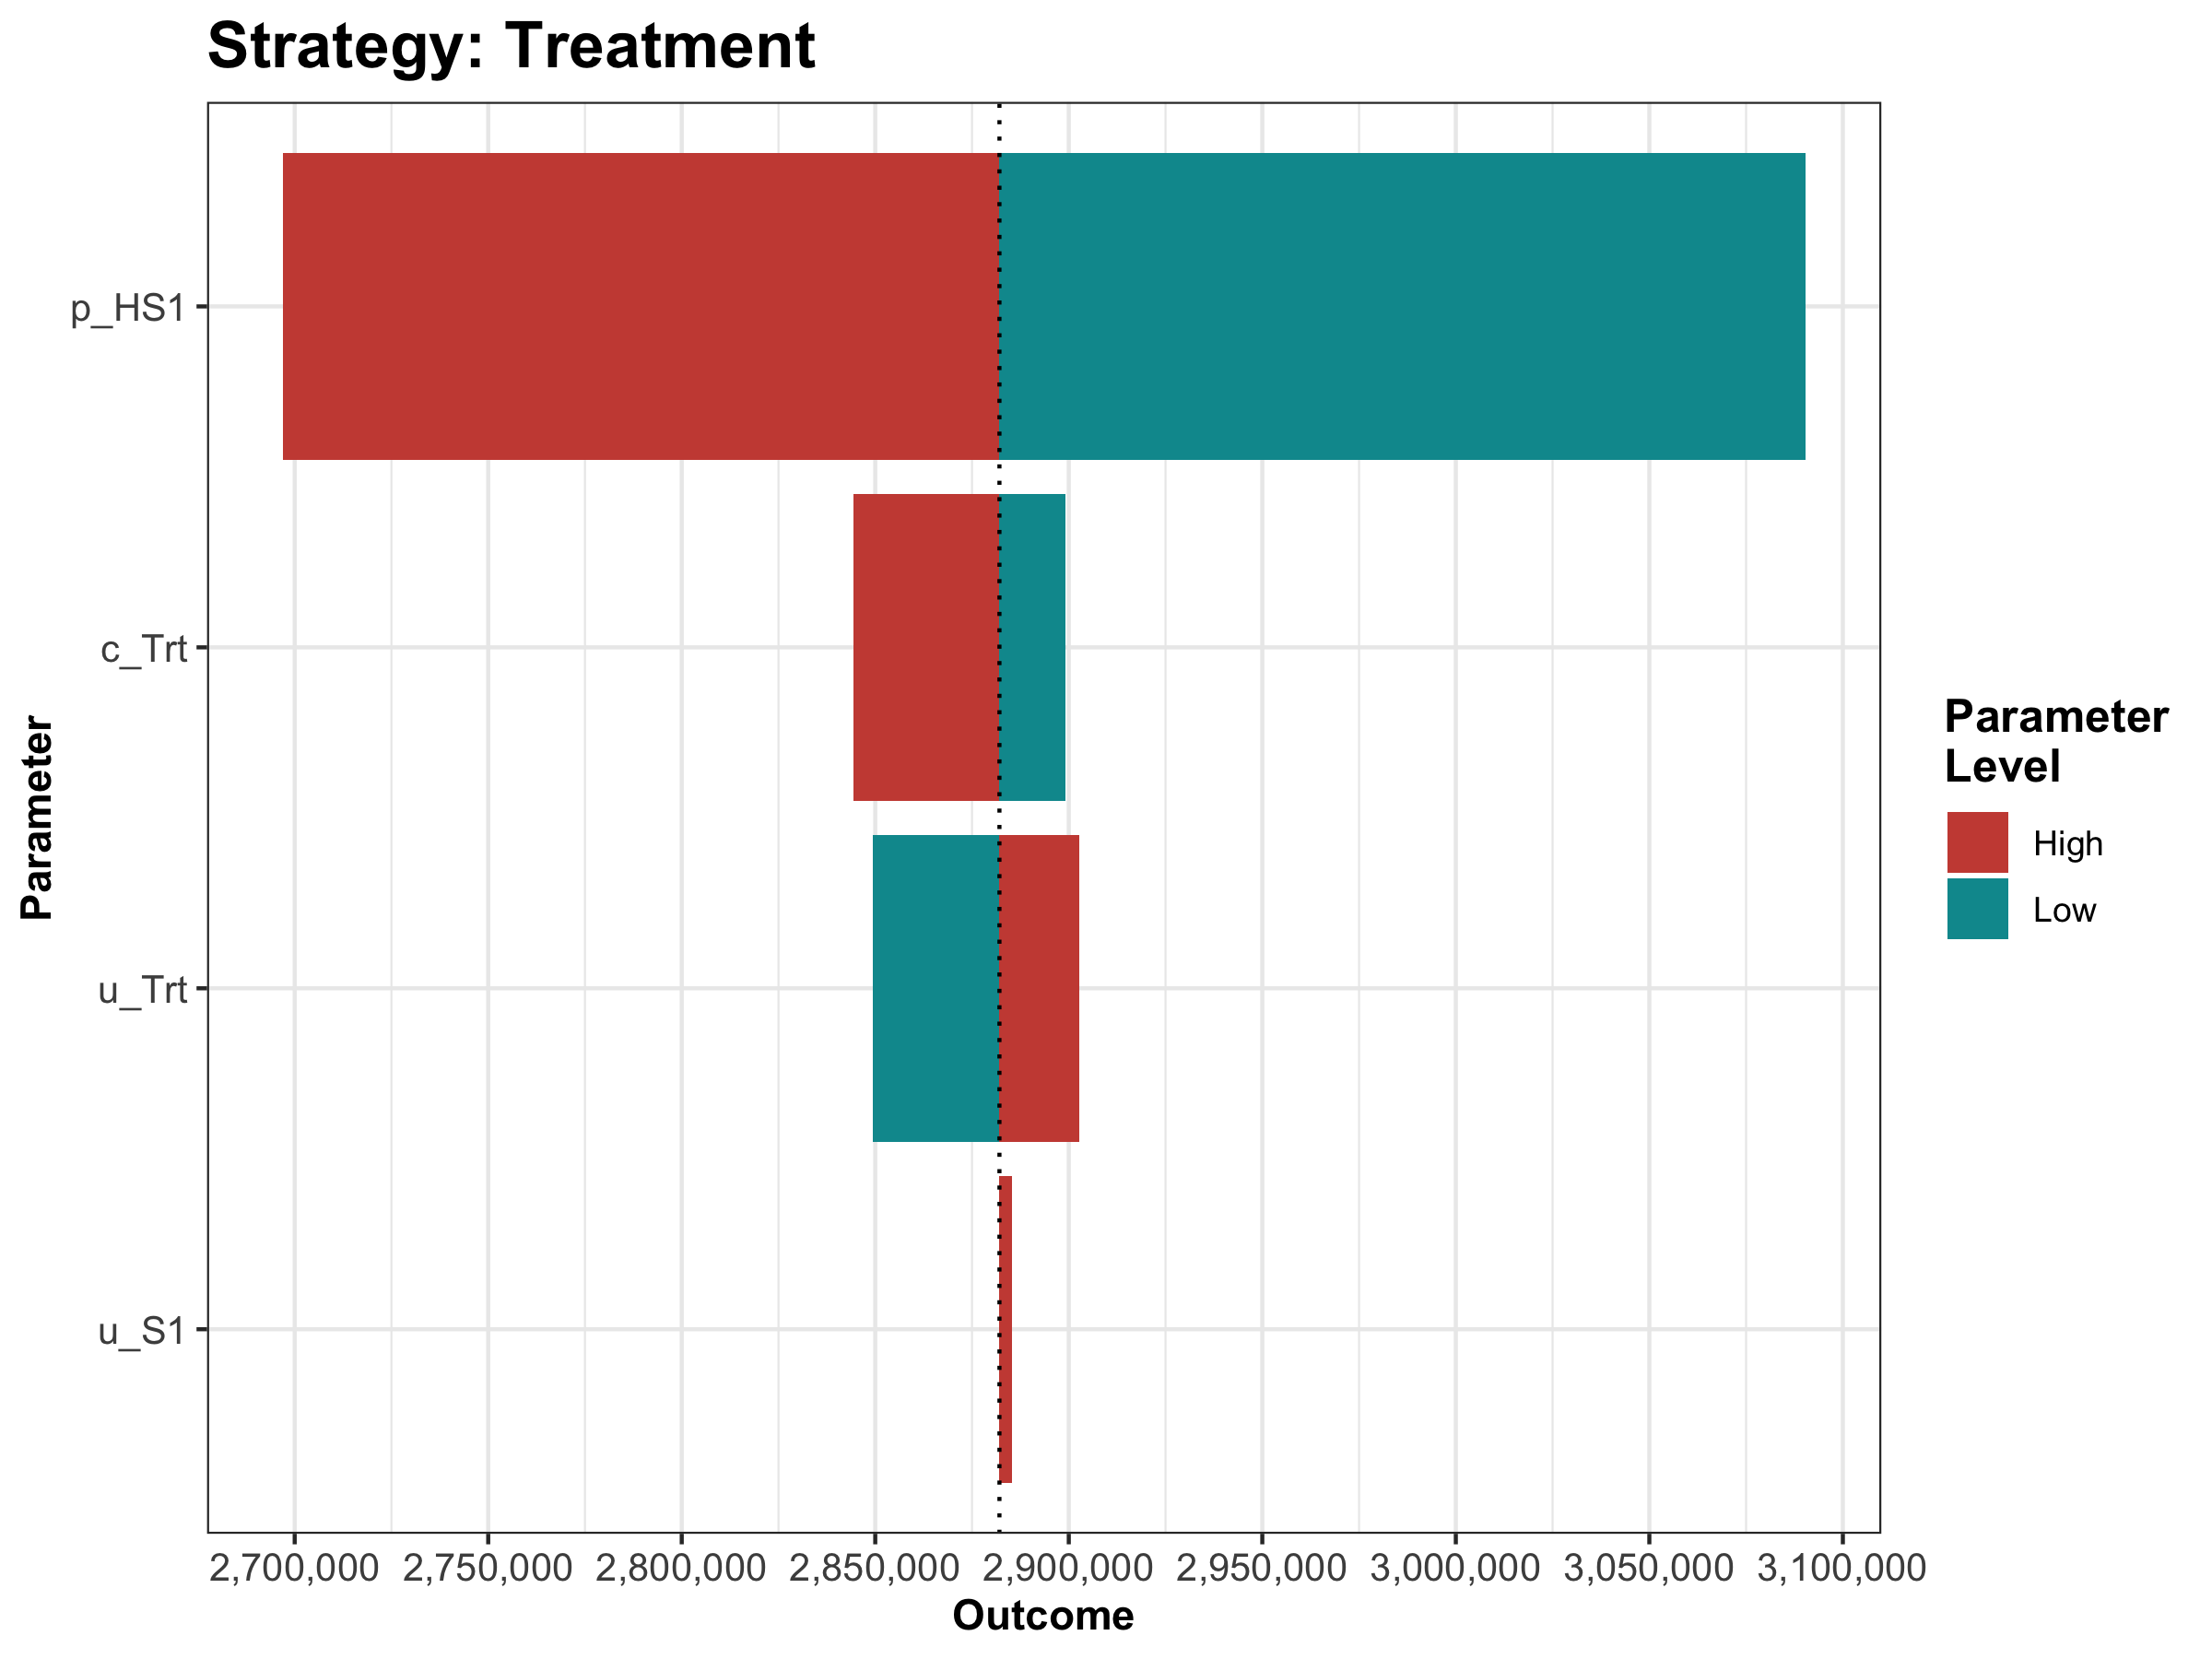
\includegraphics[width=33.33in]{../figs/05b_tornado_lrm_Treatment_nmb} 

}

\caption{Tornado plot}\label{fig:05b-tornado-lrm-Treatment-nmb}
\end{figure}

\begin{figure}

{\centering 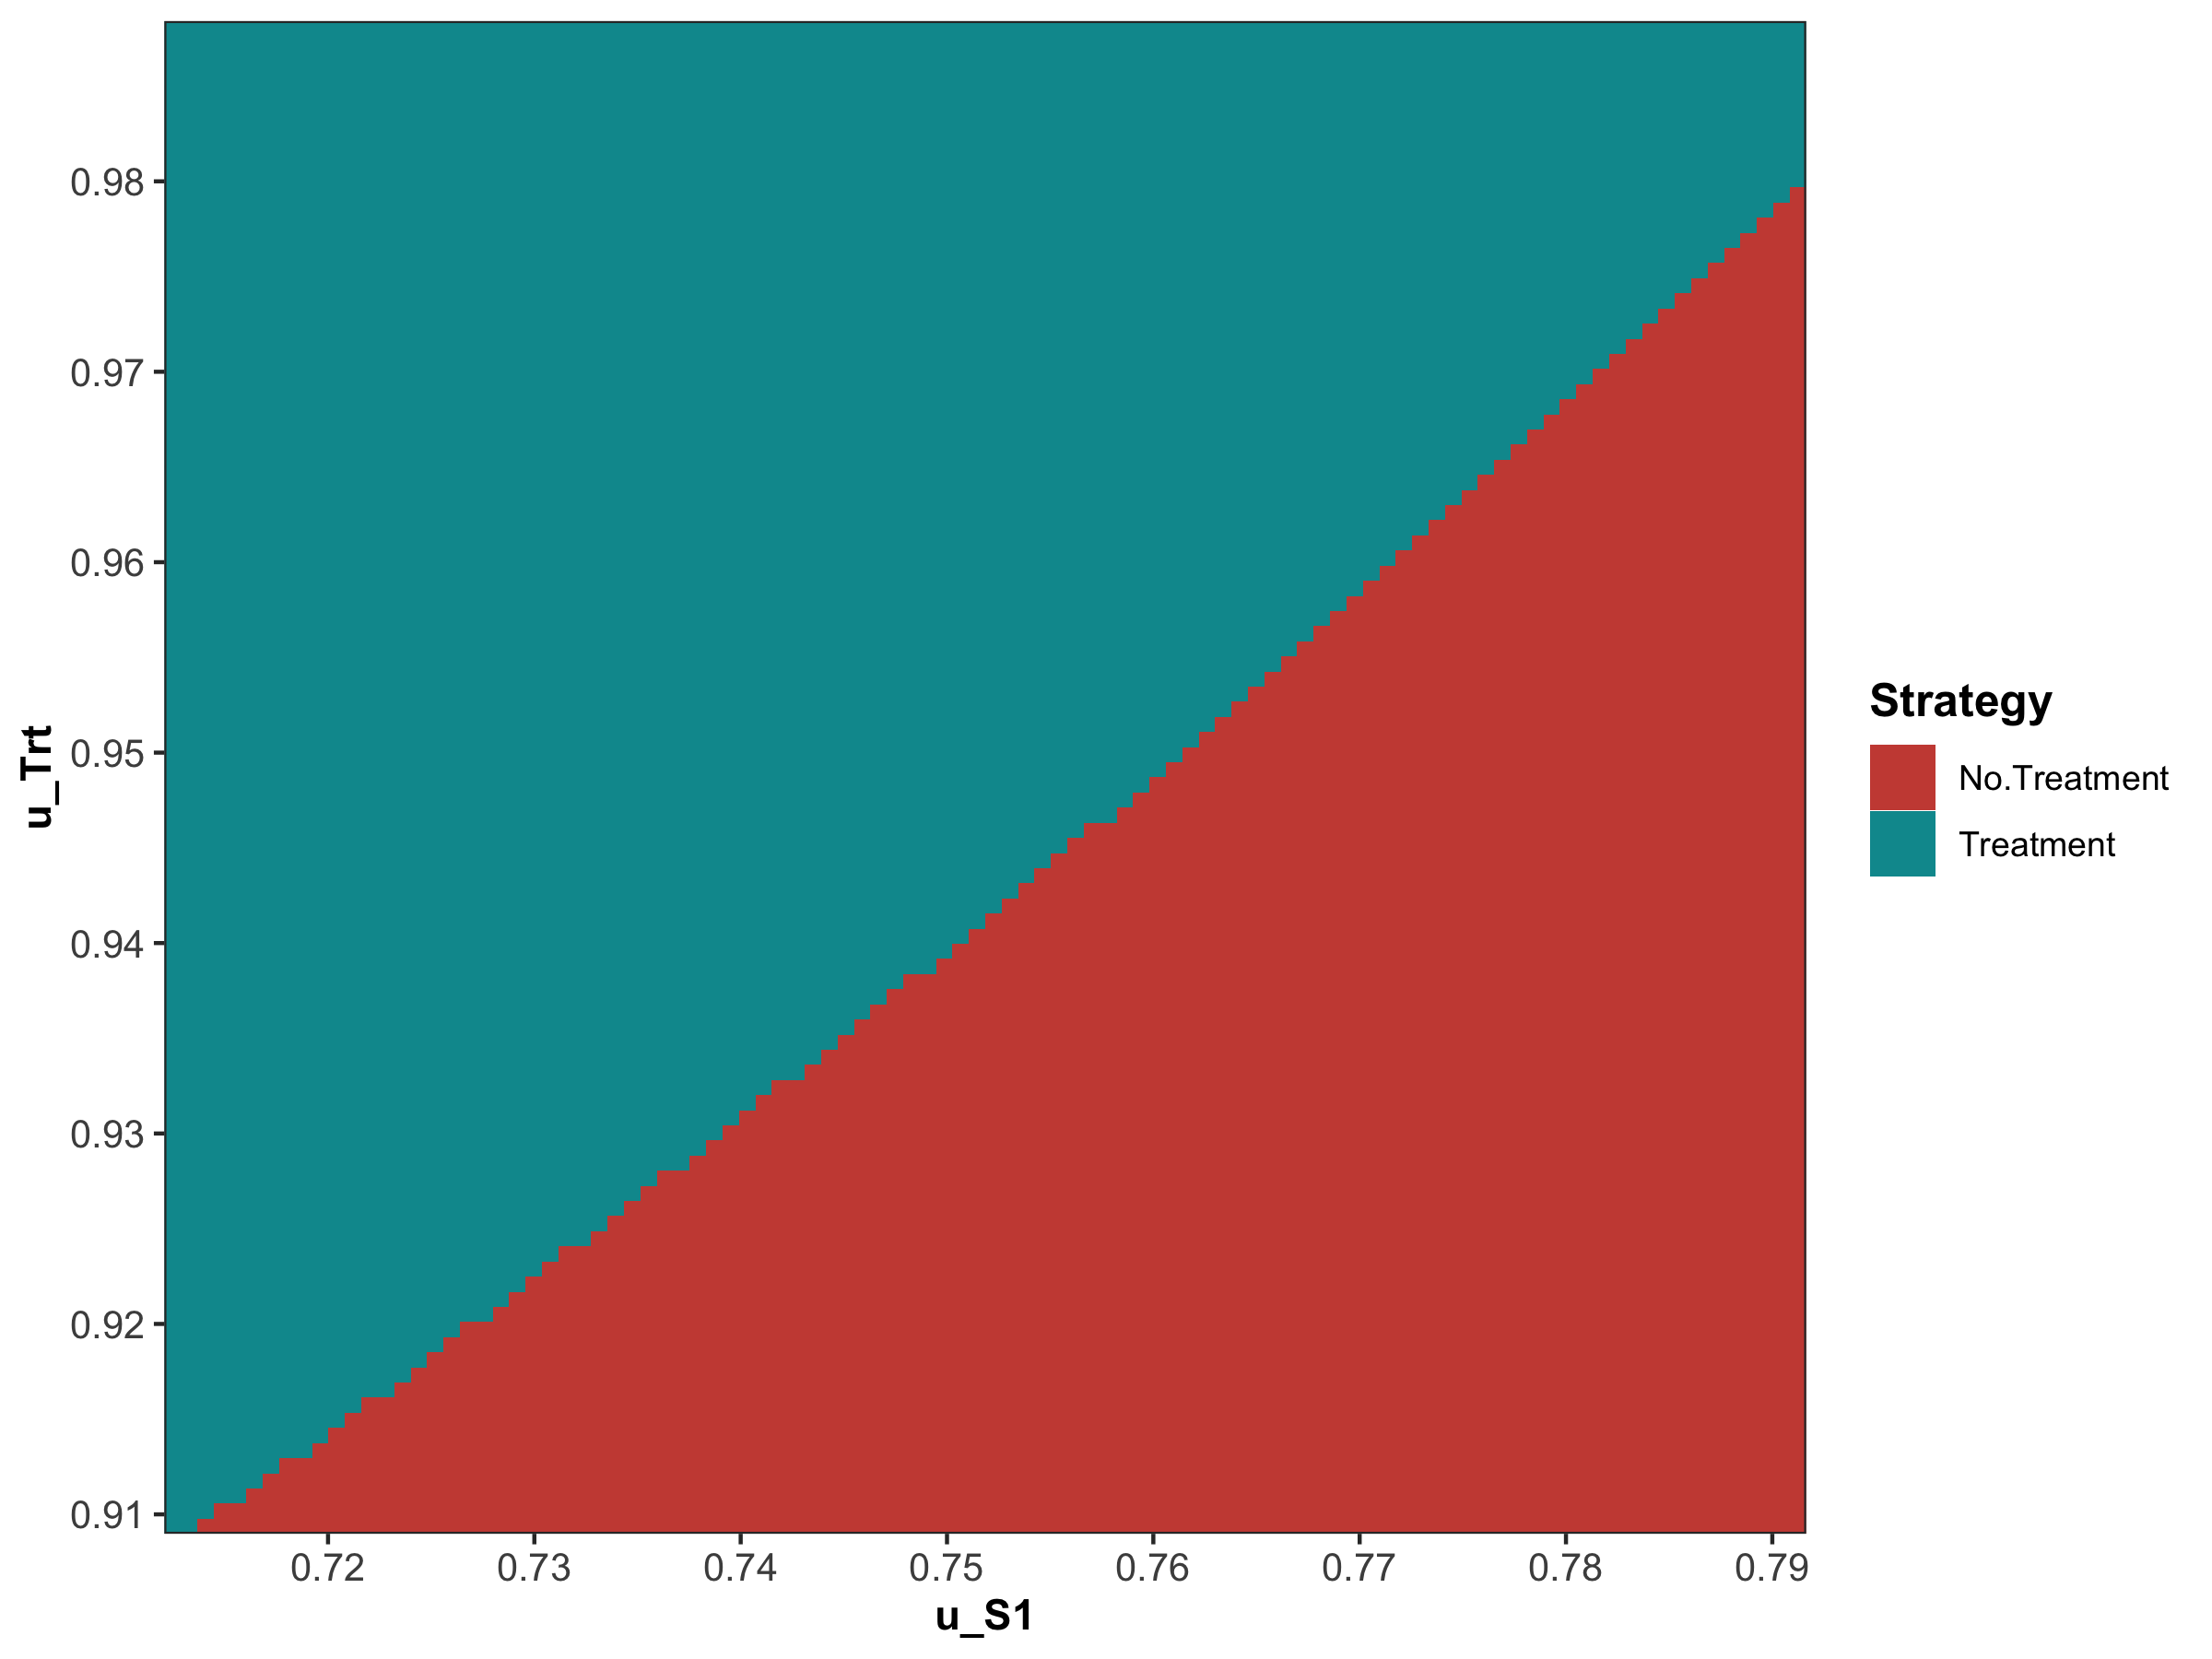
\includegraphics[width=33.33in]{../figs/05b_twsa_lrm_uS1_uTrt_nmb} 

}

\caption{Two-way sensitivity analysis (TWSA).}\label{fig:05b-twsa-lrm-uS1-uTrt-nmb}
\end{figure}

\section{05c Value of information}\label{voi}

In the VOI component, the results from the PSA generated in the
probabilistic analysis subcomponent are used to determine whether
further potential research is needed. We use the \texttt{calc\_evpi}
function from the \texttt{dampack} package to calculate the expected
value of perfect information (EVPI). Figure \ref{fig:05c-evpi} shows the
EVPI for the different WTP values.

\begin{Shaded}
\begin{Highlighting}[]
\NormalTok{evpi <-}\StringTok{ }\KeywordTok{calc_evpi}\NormalTok{(}\DataTypeTok{wtp =}\NormalTok{ v_wtp, }\DataTypeTok{psa =}\NormalTok{ l_psa)}
\end{Highlighting}
\end{Shaded}

\begin{figure}

{\centering 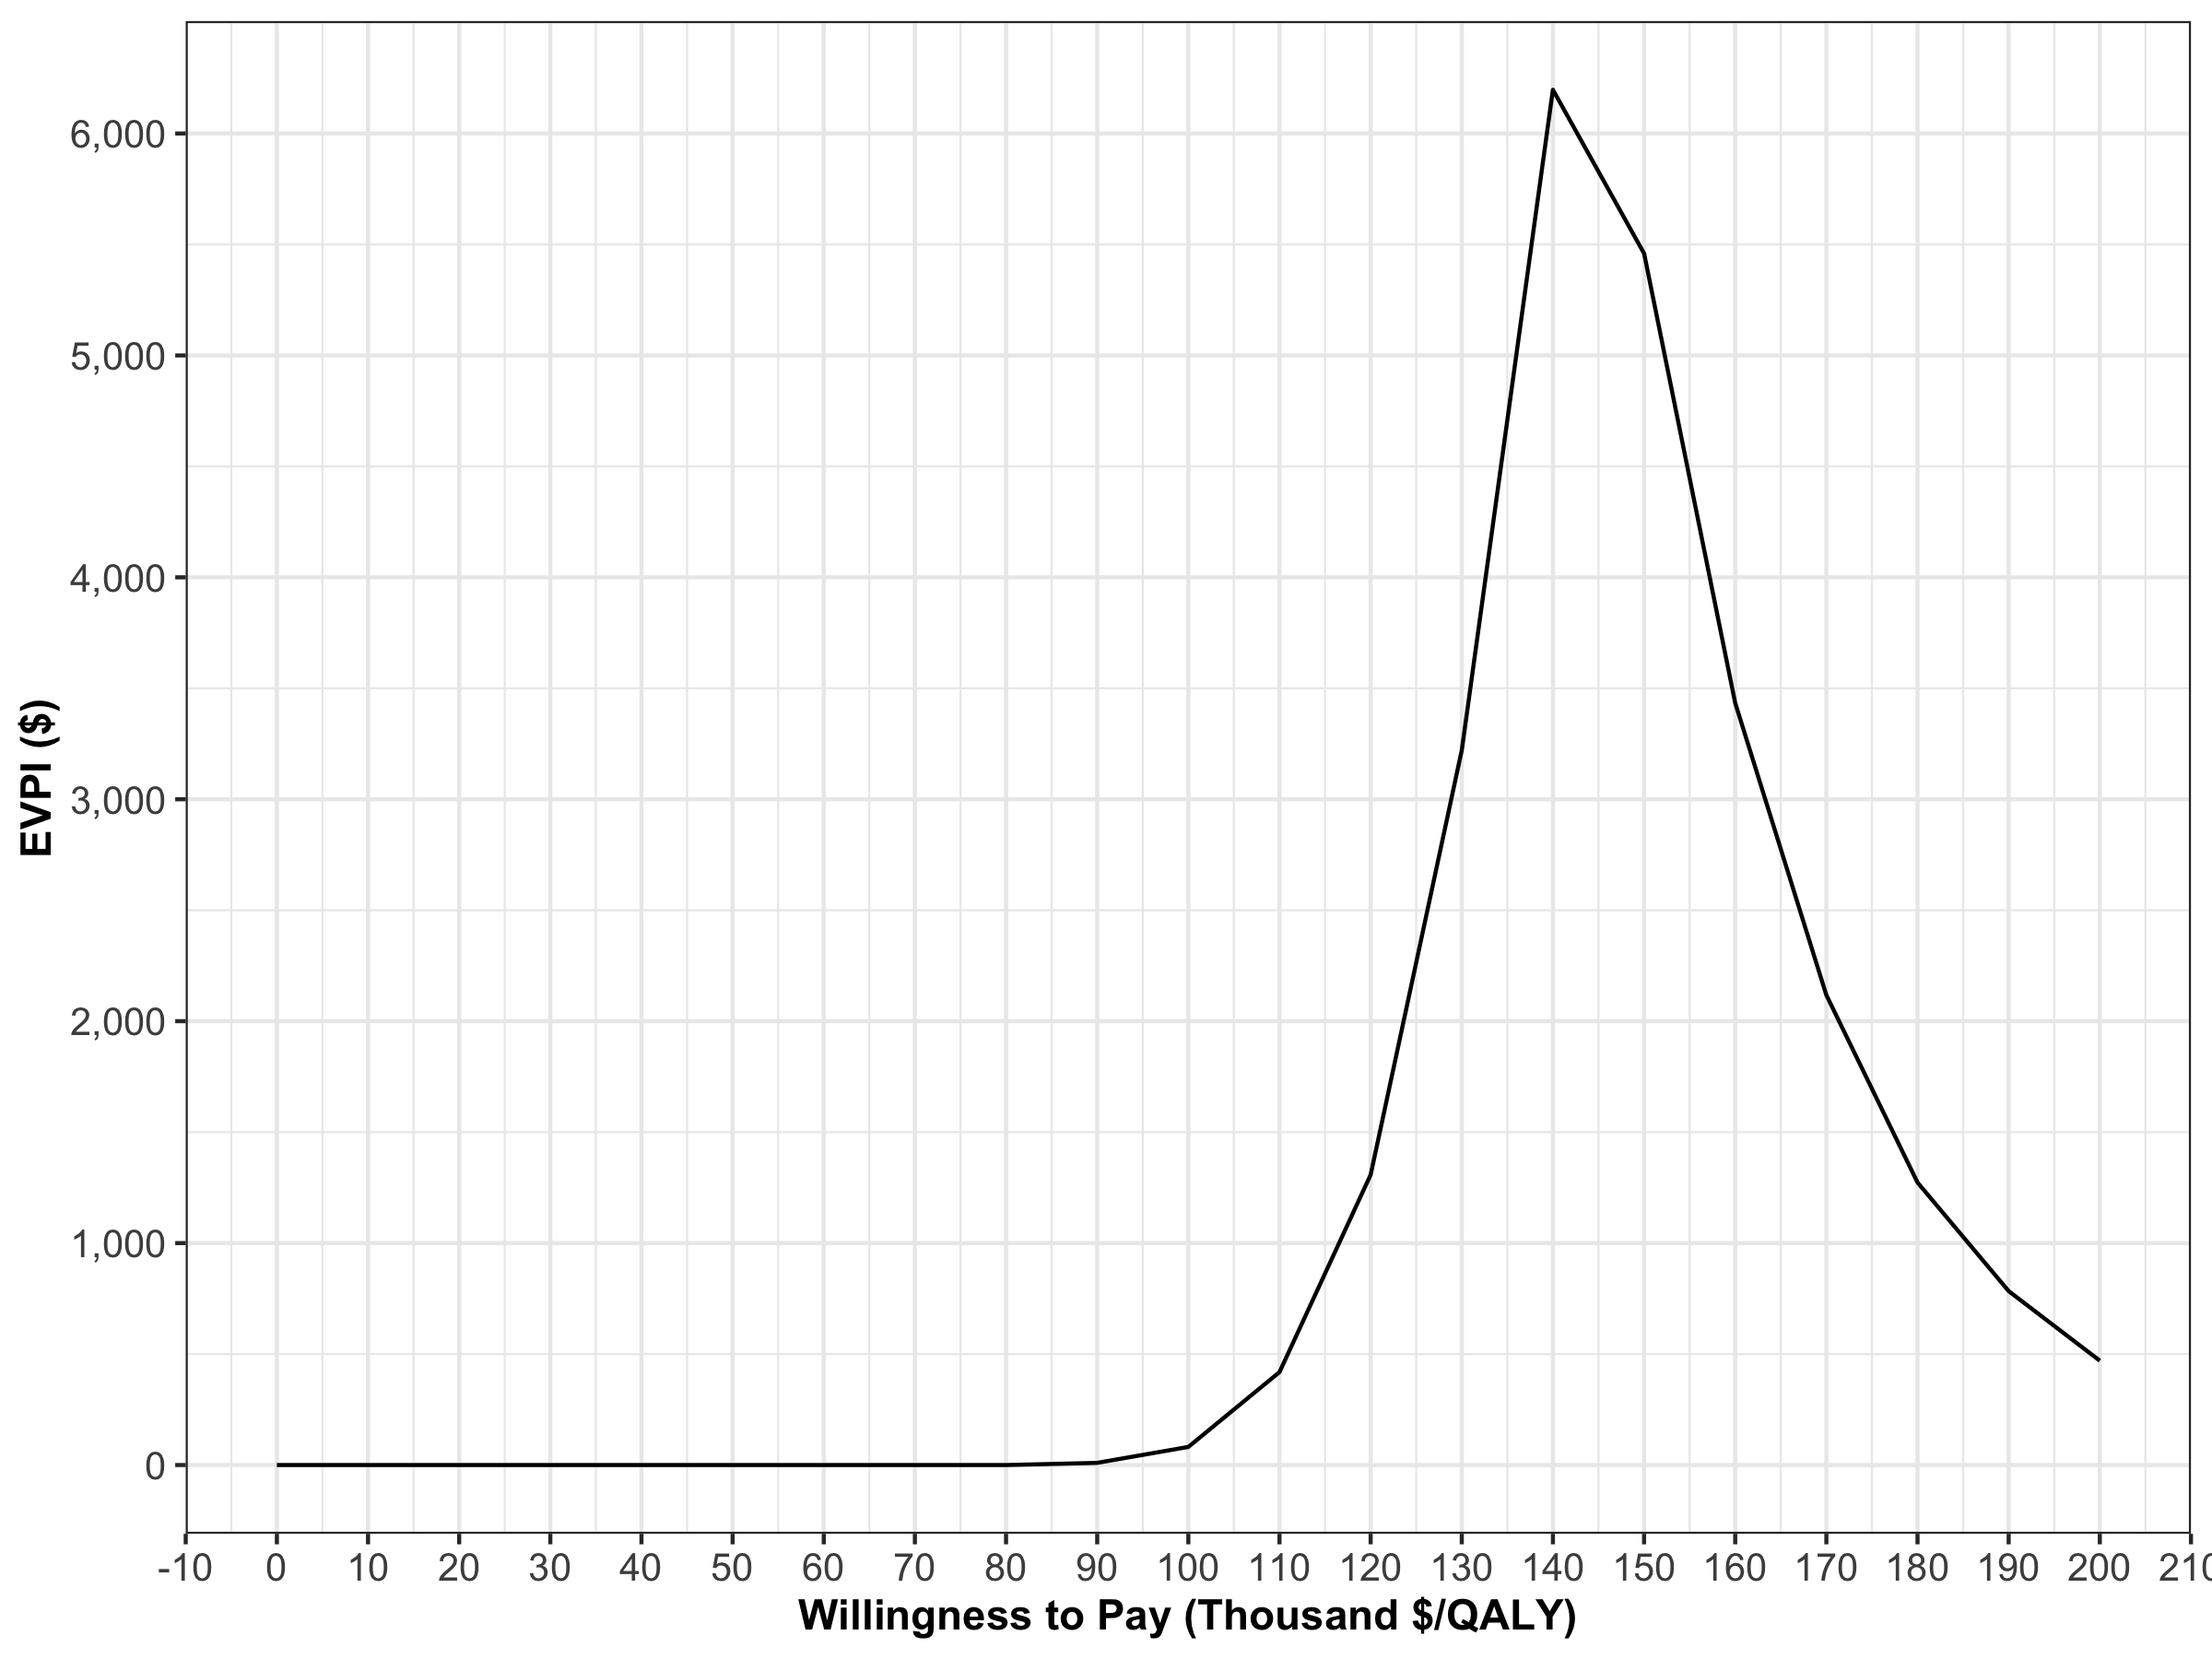
\includegraphics[width=33.33in]{../figs/05c_evpi} 

}

\caption{Expected value of perfect information}\label{fig:05c-evpi}
\end{figure}

\bibliography{book.bib,packages.bib}


\end{document}
